\documentclass[12pt,spanish,fleqn,openany,letterpaper,pagesize]{scrbook}

\usepackage[utf8]{inputenc}
\usepackage[spanish]{babel}%escribir con acentos sin necesidad de comandos \'{} .
\usepackage[version=4]{mhchem}
\usepackage{fancyhdr}
\usepackage{epsfig}
\usepackage{epic}
\usepackage{booktabs}
\usepackage{multirow}
\usepackage[table,xcdraw]{xcolor}
\usepackage{eepic}
\usepackage{amsmath}
\usepackage{threeparttable}
\usepackage{amscd}
\usepackage{here}
\usepackage{graphicx}
%\usepackage{lscape}
\usepackage{tabularx}
\usepackage{subfigure}
\usepackage{longtable}
\usepackage{cite}
\usepackage{textcomp}
%\usepackage{setspace}
\usepackage[hidelinks]{hyperref}
\usepackage{rotating} %Para rotar texto, objetos y tablas seite. No se ve en DVI solo en PS. Seite 328 Hundebuch
                        %se usa junto con \rotate, \sidewidestable ....


\renewcommand{\theequation}{\thechapter-\arabic{equation}}
\renewcommand{\thefigure}{\textbf{\thechapter-\arabic{figure}}}
\renewcommand{\thetable}{\textbf{\thechapter-\arabic{table}}}


\pagestyle{fancyplain}%\addtolength{\headwidth}{\marginparwidth}
\textheight 20.5cm \topmargin 0cm \textwidth 16.5cm %%defecto textheight 22.5cm
\oddsidemargin 0.5cm \evensidemargin 0.5cm% -0.5 even para impresión.
\renewcommand{\chaptermark}[1]{\markboth{\thechapter\; #1}{}}
\renewcommand{\sectionmark}[1]{\markright{\thesection\; #1}}
\lhead[\fancyplain{}{\thepage}]{\fancyplain{}{\rightmark}}
\rhead[\fancyplain{}{\leftmark}]{\fancyplain{}{\thepage}}
\fancyfoot{}
\thispagestyle{fancy}%


\addtolength{\headwidth}{0cm}
\unitlength1mm %Define la unidad LE para Figuras
\mathindent0cm %Define la distancia de las formulas al texto,  fleqn las descentra
\marginparwidth0cm
\parindent0cm %Define la distancia de la primera linea de un párrafo a la margen

%Para tablas,  redefine el backschlash en tablas donde se define la posición del texto en las
%casillas (con \centering \raggedright o \raggedleft)
\newcommand{\PreserveBackslash}[1]{\let\temp=\\#1\let\\=\temp}
\let\PBS=\PreserveBackslash %Espacio entre lineas
\renewcommand{\baselinestretch}{1.5}

%Neuer Befehl f\"{u}r die Tabelle Eigenschaften der Aktivkohlen
\newcommand{\arr}[1]{\raisebox{1.5ex}[0cm][0cm]{#1}}

%\onehalfspace

%Neue Kommandos
\usepackage{Befehle}
%Inicio del documento. Tener en cuenta que hay archivos auxiliares

\begin{document}
\pagenumbering{roman}
%\newpage
%\setcounter{page}{1}
\begin{center}
    \begin{figure}
        \centering%

        
\epsfig{file=HojaTitulo/LogoUPTC,scale=0.7}%
    \end{figure}
    \thispagestyle{empty} \vspace*{0.5cm} \textbf{\huge
    Evaluación de las propiedades estructurales, magnéticas y ópticas del
    sistema
    \ce{Lu_{3}Al_{5-x}Fe_{x}O_{12}}:\ce{Ce^{3+}} obtenido por método de
    reacción de
    estado sólido}\\[4cm]
    \Large\textbf{Yeison Daniel Molina Monsalve}\\[4cm]
    \small Universidad Pedagógica y Tecnológica de Colombia\\
    Facultad de Ingeniería, Maestría en metalurgia y ciencias de los
    materiales\\
    Tunja, Colombia\\
    2021\\
\end{center}

\newpage{\pagestyle{empty}}%\cleardoublepage}

\newpage
\begin{center}
    \thispagestyle{empty} \vspace*{0cm} \textbf{\huge
    Evaluación de las propiedades estructurales, magnéticas y ópticas del
    sistema
    \ce{Lu_{3}Al_{5-x}Fe_{x}O_{12}}:\ce{Ce^{3+}} obtenido por método de
    reacción de
    estado sólido}\\[1.1cm]
    \Large\textbf{Yeison Daniel Molina Monsalve}\\[1.1cm]
    \small Trabajo de grado presentado como requisito parcial para
    optar
    al
    título de:\\
    \textbf{Magister en metalurgia y ciencias de los materiales}\\[1.1cm]
    Director\\
    Carlos Arturo Parra Vargas Ph.D.\\[0.5cm]
    Codirector:\\
    Christian Fabian Olivera Varela MSc.\\[1.1cm]
    %%L\'{\i}nea de Investigación:\\
    %%Nombrar la l\'{\i}nea de investigación en la que enmarca la tesis  o trabajo de investigación\\
    Grupo de Investigación:\\
    Grupo de Física de Materiales\\[1.1cm]
    Universidad Pedagógica y Tecnológica de Colombia\\
    Facultad de Ingeniería, Maestría en metalurgia y ciencias de los
    materiales\\
    Tunja, Colombia\\
    2022\\
\end{center}

\newpage{\pagestyle{empty}}%\cleardoublepage}

\newpage
\thispagestyle{empty} \textbf{}\normalsize
\\\\\\%
\textbf{``Siempre dicen que el tiempo cambia las cosas, pero en realidad se tienen que cambiar por uno mismo\"\\\\
Andy Warhol''}\\[4.0cm]

\begin{flushright}
    \begin{minipage}{8cm}
        \noindent
        \small
        A mi madre\\
        Por inspirarme y ser mi motivación para ser cada día mejor. \\
        [1.0cm]\\
        A mi padre\\
        Por ser una gran persona, humilde y sencilla.
        \\
        
    \end{minipage}
\end{flushright}

\newpage{\pagestyle{empty}}%\cleardoublepage}

\newpage
\thispagestyle{empty} \textbf{}\normalsize
\\\\\\%
\textbf{\LARGE Agradecimientos}
\phantomsection
\addcontentsline{toc}{chapter}{\numberline{}Agradecimientos}\\\\

Agradezco al doctor Carlos Parra por permitirme desarrollar mi trabajo de grado de maestría 
en el grupo de Investigación de Física de Materiales de la Universidad Pedagógica y Tecnológica de Colombia, 
y a su equipo de trabajo por su colaboración y asesoría en el desarrollo de esta investigación, 
especialmente a Christian Varela por su dedicación, acompañamiento y esmero.
%Esta sección es opcional, en ella el autor agradece a las personas o
%instituciones que colaboraron en la realización de la tesis  o trabajo de
%investigación. Si se incluye esta sección, deben aparecer los nombres
%completos, los cargos y su aporte al documento.\\

\newpage{\pagestyle{empty}}%\cleardoublepage}

\newpage
\textbf{\LARGE Resumen}
\phantomsection
\addcontentsline{toc}{chapter}{\numberline{}Resumen}\\\\

El granate de aluminio lutecio (LuAG), presenta una estructura prometedora como
anfitrión de diferentes tierras raras, permitiendo su aplicación en diferentes
dispositivos debido a sus propiedades ópticas. El LuAG dopado con \ce{Ce^{3+}} es
un fósforo de color amarillo, ampliamente utilizado como conversor en diodos emisores
de luz (LED). En el presente trabajo se obtuvo una nueva serie de granates 
\ce{Lu_{3}Al_{5-x}Fe_{x}O_{12}}:\ce{Ce^{3+}} ($0.0 \leq x \leq 4.5$)
mediante el método de reacción en estado sólido a 1200 \textcelsius. Los
materiales
obtenidos se caracterizaron por difracción de rayos X, refinamiento de
Rietveld, espectroscopía de reflectancia difusa UV-Vis, espectroscopía de
absorción, espectroscopía de fotoluminiscencia, microscopia electrónica de
barrido (SEM),
EDX y magnetometría de muestra vibrante (VSM). El dopaje con \ce{Fe^{3+}}
permitió
obtener materiales en fase pura a temperaturas y tiempos por debajo de los
reportados anteriormente. Por otro lado, los materiales alcanzaron una
absorción
de azul mejorada y una emisión ajustable de verde a naranja. Estas
propiedades ópticas son atribuibles a un fenómeno de desplazamiento hacia el
rojo debido a un aumento de la división del campo cristalino en los niveles de
energía de \ce{Ce^{3+}}. Además, los fósforos obtenidos exhibieron un alto
rendimiento
cuántico (55$-$67\%), excelente estabilidad de fotoluminiscencia térmica (hasta
200\textcelsius) y alta conversión de color, lo que hace que los fósforos
obtenidos
sean candidatos prometedores para aplicación en la fabricación de w-LED.\\

Debido al dopaje del granate anfitrión LuAG:Ce con iones \ce{Fe^{3+}} se
observó un
aumento en el tamaño de la red cristalina y de partícula, también permitió
generar propiedades magnéticas,
partiendo de una respuesta paramagnética a ferrimagnética, con un valor de
magnetización de saturación de $\sim$
10 emu/g a un campo aplicado relativamente bajo de $\sim$ 1500 Oe.

%El estudio presenta el proceso de sinterización del sistema
%\ce{Lu3Al_{5-x}Fe_{x}O_{12}}:\ce{Ce^{3+}} por método
%de reacción de estado sólido, el análisis realizado de las propiedades
%estructurales, ópticas, morfológicas, composicionales y magnéticas,
%mediante la caracterización usando técnicas de difracción de rayos X,
%refinamiento Rietveld, reflectancia difusa, absorción óptica,
%fotoluminiscencia, eficiencia Cuántica, microscopia electrónica de barrido
%(MEB) y magnetometría de muestra vibrante (VSM) Evaluar el efecto de la
%inclusión del catión Fe3+ sobre las propiedades
%estructurales, magnéticas y ópticas de los óxidos mixtos obtenidos.\\

%Se evaluó el efecto que tuvo la inclusión del ión \ce{Fe^{3+}} dentro de la
%estructura del granate LuAG sobre las propiedades
%estructurales, ópticas y magnéticas; empleando el sistema
%\ce{Lu3Al_{5-x}Fe_{x}O_{12}}:\ce{Ce^{3+}} con $0.0 \leq x \leq 4.5$.\\

%La investigación experimental que permitió conocer la influencia del
%\ce{Fe^{3+}} sobre las alteraciones en la propiedades del granate LuAG

%El resumen es una presentación abreviada y precisa (la NTC 1486 de 2008
%recomienda revisar la norma ISO 214 de 1976). Se debe usar una extensión
%máxima de 12 renglones. Se recomienda que este resumen sea analítico,
%es decir, que sea completo, con información cuantitativa y cualitativa,
%generalmente incluyendo los siguientes aspectos: objetivos, diseño, lugar y
%circunstancias, pacientes (u objetivo del estudio), intervención,
%mediciones y principales resultados, y conclusiones. Al final del resumen se
%deben usar palabras claves tomadas del texto (mínimo 3 y máximo 7
%palabras), las cuales permiten la recuperación de la información.\\

%\textbf{\small Palabras clave: (máximo 10 palabras, preferiblemente
%seleccionadas de las listas internacionales que permitan el indizado
%cruzado)}.\\

%A continuación se presentan algunos ejemplos de tesauros que se pueden
%consultar para asignar las palabras clave, seg\'{u}n el \'{a}rea
%temática:\\

%\textbf{Artes}: AAT: Art y Architecture Thesaurus.

%\textbf{Ciencias agropecuarias}: 1) Agrovoc: Multilingual Agricultural
%Thesaurus - F.A.O. y 2)GEMET: General Multilingual Environmental Thesaurus.

%\textbf{Ciencias sociales y humanas}: 1) Tesauro de la UNESCO y 2) Population
%Multilingual Thesaurus.

%\textbf{Ciencia y tecnología}: 1) Astronomy Thesaurus Index. 2) Life
%Sciences Thesaurus, 3) Subject Vocabulary, Chemical Abstracts Service y 4)
%InterWATER: Tesauro de IRC - Centro Internacional de Agua Potable y
%Saneamiento.

%\textbf{Tecnologías y ciencias médicas}: 1) MeSH: Medical Subject
%Headings (National Library of Medicine's USA) y 2) DECS: Descriptores en
%ciencias de la Salud (Biblioteca Regional de Medicina BIREME-OPS).

%\textbf{Multidisciplinarias}: 1) LEMB - Listas de Encabezamientos de Materia y
%2) LCSH- Library of Congress Subject Headings.\\

%También se pueden encontrar listas de temas y palabras claves, consultando
%las distintas bases de datos disponibles a través del Portal del Sistema
%Nacional de Bibliotecas\footnote{ver: www.sinab.unal.edu.co}, en la sección
%"Recursos bibliográficos" opción "Bases de datos".\\

%\textbf{\LARGE Abstract}\\\\
%Es el mismo resumen pero traducido al inglés. Se debe usar una
%extensión máxima de 12 renglones. Al final del Abstract se deben
%traducir las anteriores palabras claves tomadas del texto (mínimo 3 y
%máximo 7 palabras), llamadas keywords. Es posible incluir el resumen en
%otro idioma diferente al español o al inglés, si se considera como
%importante dentro del tema tratado en la investigación, por ejemplo: un
%trabajo dedicado a problemas lingüísticos del mandarín
%seguramente estar\'{\i}a mejor con un resumen en mandar\'{\i}n.\\[2.0cm]
%\textbf{\small Keywords: palabras clave en inglés(máximo 10 palabras,
%preferiblemente seleccionadas de las listas internacionales que permitan el
%indizado cruzado)}\\

\renewcommand{\tablename}{\textbf{Tabla}}
\renewcommand{\figurename}{\textbf{Figura}}
\renewcommand{\listtablename}{Lista de Tablas}
\renewcommand{\listfigurename}{Lista de Figuras}
\renewcommand{\contentsname}{Contenido}

%\newcommand{\clearemptydoublepage}{\newpage{\pagestyle{empty}\cleardoublepage}}
%\cleardoublepage{}
\phantomsection
\addcontentsline{toc}{chapter}{Lista de figuras} % para que aparezca en el indice de contenidos
\listoffigures % indice de figuras

%\cleardoublepage{}
\phantomsection
\addcontentsline{toc}{chapter}{Lista de tablas} % para que aparezca en el indice de contenidos
\listoftables % indice de tablas

%\cleardoublepage{}
%\addcontentsline{toc}{chapter}{Contenido} % para que aparezca en el indice de contenidos
\tableofcontents % indice de tablas

%\chapter*{Lista de s\'{\i}mbolos}
\addcontentsline{toc}{chapter}{\numberline{}Lista de s\'{\i}mbolos}
Esta secci\'{o}n es opcional, dado que existen disciplinas que no manejan s\'{\i}mbolos y/o abreviaturas.\\

Se incluyen s\'{\i}mbolos generales (con letras latinas y griegas), sub\'{\i}ndices, super\'{\i}ndices y abreviaturas (incluir s\'{o}lo las clases de s\'{\i}mbolos que se utilicen). Cada una de estas listas debe estar ubicada en orden alfab\'{e}tico de acuerdo con la primera letra del s\'{\i}mbolo.
\section*{S\'{\i}mbolos con letras latinas}
 \label{simbolos}
 \renewcommand{\arraystretch}{1.3}
%\begin{longtable}[l]{*{4}{>{$}l<{$}}p{9cm}}
\begin{longtable}[l]{>{$}l<{$}l>{$}l<{$}>{$}l<{$}}
%\begin{tabular}
\textbf{S\'{\i}mbolo}&\textbf{T\'{e}rmino}&\textbf{Unidad SI}&\textbf{Definici\'{o}n}\\[0.5ex]\hline
\endfirsthead%
\textbf{S\'{\i}mbolo}&\textbf{T\'{e}rmino}&\textbf{Unidad SI}&\textbf{Definici\'{o}n}\\[0.5ex]\hline
\endhead%
      A              &\'{A}rea                                   &\text{m}^{2}                         &\int\int dxdy\\%
      A_{\text{BET}} &\'{A}rea interna del s\'{o}lido                &\frac{\text{m}^{2}}{\text{g}}        &\text{ver DIN ISO 9277}\\%
      A_{\text{g}}   &\'{A}rea transversal de la fase gaseosa    &\text{m}^{2}                         &\text{Ec...}\\%
      A_{\text{s}}   &\'{A}rea transversal de la carga a granel  &\text{m}^{2}                         &\text{Ec...}\\%
      a              &Coeficiente                            &1                                    &\text{Ec...}\\%
      a              &Contenido de ceniza                    &1                                    &\frac{m_{\text{ceniza}}}{m_{\text{bm,0}}}\\%
      c              &Contenido de carbono                   &1                                    &\frac{m_{\text{C}}}{m}\\%
      c              &Longitud de la cuerda                  &\text{m}                             &\text{Figura...}\\
      c              &Concentraci\'{o}n de la cantidad de materia&\frac{\text{mol}}{\text{m}^{3}}      &\frac{n}{V}\\%
      D              &Di\'{a}metro                               &\text{m}                             &\\%
      E_{\text{A}}   &Energ\'{\i}a de activaci\'{o}n                  &\frac{\text{kJ}}{\text{mol}}         &\text{Ec....}\\%
      F              &Fracci\'{o}n de materia vol\'{a}til            &1                                    &\text{ver DIN 51720}\\%
      Fr             &N\'{u}mero de Froude                       &1                                    &\frac{\omega^{2}R}{g_{\text{0}}}\\%
      \overrightarrow{g}&Aceleraci\'{o}n de la gravedad          &\frac{\text{m}}{\text{s}^{2}}        &\frac{d^{2}\overrightarrow{r}}{dt^{2}}\\%
      H              &Entalp\'{\i}a                               &\text{J}                             &U+PV\\%
      H_{\text{o}}   &Poder calor\'{\i}fico superior              &\frac{\text{MJ}}{\text{kg}}          &\text{ver DIN 51857}\\%
      h              &Contenido de hidr\'{o}geno                 &1                                    &\frac{m_{\text{H}}}{m}\\%
      K              &Coeficiente de equilibrio              &1                                    &\text{Ec...}\\%
      L              &Longitud                               &\text{m}                             &DF\\%
      L              &Longitud del reactor                   &\text{m}                             &\text{Figura...}\\%
      m              &Masa                                   &\text{kg}                            &DF\\%
      \dot{m}        &Flujo de masa                          &\frac{\text{kg}}{\text{s}}           &\frac{m}{t}\\%
      n              &Velocidad de rotaci\'{o}n                  &\frac{\text{1}}{\text{s}}            &\frac{\omega}{2\pi}\\%
      n              &Cantidad de materia                    &\text{mol}                           &DF\\%
      P              &Presi\'{o}n                                &\text{Pa}                            &\frac{\vec{F}\cdot\vec{n}}{A}\\%
      Q              &Calor                                  &\text{kJ}                            &\text{1. $LT$}\\%
      T              &Temperatura                            &\text{K}                             &DF\\%
      t              &Tiempo                                 &\text{s}                             &DF\\%
      x_{\text{i}}   &Fracci\'{o}n de la cantidad de materia     &1                                    &\frac{n_{\text{i}}}{n}\\%
      V              &Volumen                                &\text{m}^{3}                         &\int{dr^{3}}\\%
      \vec{u}        &Velocidad                              &\frac{\text{m}}{\text{s}}            &(\frac{dr}{dt},r\frac{d\upsilon}{dt},\frac{dz}{dt})\\%
      w_{\text{i}}   &Fracci\'{o}n en masa del componente i      &1                                    &\frac{m_{\text{i}}}{m_{\text{0}}}\\%
      w_{\text{w,i}} &Contenido de humedad de la sustancia i &1                                    &\frac{m_{\text{\wasser}}}{m_{\text{i,0}}}\\%
      Z              &Factor de gases reales                 &1                                    &\frac{pv}{RT}\\%
\end{longtable}
\vspace{5ex}
\section*{S\'{\i}mbolos con letras griegas}

\begin{longtable}[l]{>{$}l<{$}l>{$}l<{$}>{$}l<{$}}
\textbf{S\'{\i}mbolo}&\textbf{T\'{e}rmino}&\textbf{Unidad SI}&\textbf{Definici\'{o}n}\\[0.5ex] \hline%
\endfirsthead%
\textbf{S\'{\i}mbolo}&\textbf{T\'{e}rmino}&\textbf{Unidad SI}&\textbf{Definici\'{o}n}\\[0.5ex] \hline%
\endhead%
\renewcommand{\arraystretch}{1.3}
 \label{simbolosg}
     \alpha_{\text{BET}}  &Factor de superficie                  &\frac{\text{m}^{2}}{\text{g}}   &(w_{\text{F,waf}})(A_{\text{BET}})\\%
     \beta_{\text{i}}     &Grado de formaci\'{o}n del componente i   &1                               &\frac{m_{\text{i}}}{m_{\text{bm,0}}}\\%
     \gamma               &Wandhaftreibwinkel (Stahlblech)       &1                               &\text{Secci\'{o}n...}\\
     \epsilon             &Porosidad de la part\'{\i}cula             &1                               &1-\frac{\rho_{\text{s}}}{\rho_{\text{w}}}\\%
     \eta                 &mittlere Bettneigungswinkel (St\"{u}rzen) &1                               &\text{Figura...}\\%
     \theta               &\'{A}ngulo de inclinaci\'{o}n de la cama      &1                               &\text{Figura...}\\
     \theta_{\text{O}}    &\'{A}ngulo superior de avalancha          &1                               &\text{Figura...}\\
     \theta_{\text{U}}    &\'{A}ngulo inferior de avalancha          &1                               &\text{Figura...}\\
     \kappa               &Velocidad de calentamientoe           &\frac{\text{K}}{\text{s}}       &\frac{dT}{dt}\\%
     \nu                  &Coeficiente estequiom\'{e}trico           &1                               &\text{ver DIN 13345}\\%
     \rho_{\text{b}}      &Densidad a granel                     &\frac{\text{kg}}{\text{m}^{3}}  &\frac{m_{\text{S}}}{V_{\text{S}}}\;(\text{Secci\'{o}n...})\\
     \rho_{\text{s}}      &Densidad aparente                     &\frac{\text{kg}}{\text{m}^{3}}  &\frac{m_{\text{F}}}{V_{\text{P}}}\;(\text{Secci\'{o}n...})\\
     \rho_{\text{w}}      &Densidad verdadera                    &\frac{\text{kg}}{\text{m}^{3}}  &\frac{m_{\text{F}}}{V_{\text{F}}}\;(\text{Secci\'{o}n...})\\
     \tau                 &Tiempo adimensional                   &1                               &\text{Ec....}\\%
     \Phi_{\text{V}}      &Flujo volum\'{e}trico                     &\frac{\text{m}^{3}}{\text{s}}   &\frac{\Delta V}{\Delta t}\\
     \omega               &Velocidad angular                     &\frac{1}{\text{s}}              &\frac{d\upsilon}{dt}\\

\end{longtable}


\section*{Sub\'{\i}ndices}
\begin{longtable}[l]{>{}l<{}l}
  \textbf{Sub\'{\i}ndice} & \textbf{T\'{e}rmino} \\[0.5ex] \hline%
  \endfirsthead%
  \textbf{Sub\'{\i}ndice} & \textbf{T\'{e}rmino} \\[0.5ex] \hline%
  \endhead%
\renewcommand{\arraystretch}{1.4}\label{simbolosg}

 bm&materia org\'{a}nica\\%
 DR&Dubinin-Radushkevich\\%
 E&Experimental\\%
 g&Fase gaseosa\\%
 k&Condensado\\%
 Ma&Macroporos\\%
 P&Part\'{\i}cula\\%
 p&Poro\\%
 p&Pirolizado\\%
 R&Reacci\'{o}n\\%
 t&Total\\%
 wf&Libre de agua\\%
 waf&Libre de agua y de ceniza\\%
 0&Estado de referencia\\%

\end{longtable}


\setlength{\extrarowheight}{0pt}


\section*{Super\'{\i}ndices}
\begin{longtable}[l]{>{}l<{}l}
  \textbf{Super\'{\i}ndice} & \textbf{T\'{e}rmino} \\[0.5ex] \hline%
  \endfirsthead%
  \textbf{Super\'{\i}ndice} & \textbf{T\'{e}rmino} \\[0.5ex] \hline%
  \endhead%
\renewcommand{\arraystretch}{1.4}\label{simbolosg}

 n &Coeficiente x\\%



\end{longtable}


\setlength{\extrarowheight}{0pt}


\section*{Abreviaturas}
\begin{longtable}[l]{>{}l<{}l}
  \textbf{Abreviatura} & \textbf{T\'{e}rmino} \\[0.5ex] \hline%
  \endfirsthead%
  \textbf{Abreviatura} & \textbf{T\'{e}rmino} \\[0.5ex] \hline%
  \endhead%
\renewcommand{\arraystretch}{1.4}\label{simbolosg}
 1.$LT$&Primera ley de la termodin\'{a}mica\\%
 $DF$    &Dimensi\'{o}n fundamental\\%
 $RFF$   &Racimos de fruta fresca\\%

\end{longtable}


\setlength{\extrarowheight}{0pt}
%\include{Resumen}%\newcommand{\clearemptydoublepage}{\newpage{\pagestyle{empty}\cleardoublepage}}
\pagenumbering{arabic}
\chapter{Introducción}
La luz es la parte de espectro electromagnético que puede ser percibida por el
ojo humano, esta tiene impacto sobre la vida sin importar de que fuente
provenga. A finales del siglo XIX y principios del siglo XX se dieron avances
científicos y tecnológicos en la óptica que dieron paso al desarrollo tecnológico
de fuentes artificiales entre las que incluyen, la bombilla incandescente,
seguido de otras fuentes de iluminación como, las lámparas fluorescentes,
halógenas, los diodos Emisores de Luz y recientemente los LED orgánicos\cite{Sustentable2014}.
Cada una de estas tecnologías de iluminación ha
experimentado un cambio constante debido a mejoras en los materiales,
diseño, calidad de luz, eficiencia energética y la eficiencia en el proceso de
fabricación. Desde sus inicios hasta la actualidad, la iluminación de estado
sólido ha sido líder en la industria de la iluminación, en donde,
los dispositivos más conocidos y ampliamente empleados son los LED combinados
con fósforos\cite{ISR-UniversidaddeCoimbra2017,Bernal2016}.\\

En la actualidad no existe ningún LED capaz de generar directamente luz blanca. 
En el diodo emisor de luz blanca (wLED), se obtiene mediante la mezcla de
varios colores, que
se obtiene de la combinación de emisión de luz azul y un fósforo amarillo,
sin embargo, los wLED no pueden alcanzar potencias altas de manera nativa,
debido a que, la naturaleza del funcionamiento de estos dispositivos
les impide mantener
su eficiencia a altas densidades de corriente eléctrica. Los diodos
láser (LD) pueden alcanzar potencias elevadas sin perder eficiencia, pero esto
conlleva a otra dificultad y es la degradación del fósforo. Por lo tanto,
se suele incorporar los fósforos en resinas orgánicas, pero estos
materiales no son capaces de resistir la potencia de un LD. Por lo tanto, es
necesario emplear materiales más resistentes, por ejemplo, los materiales
cerámicos que presentan una mejor conductividad térmica y estabilidad química a
temperaturas mayores que las resinas\cite{AlvarezJauregui2020}, permitiendo que los diodos
emisores de luz tengan aplicaciones tanto para baja potencia como alta
potencia, por lo que se usan con gran frecuencia en la industria de comunicación,
alimentos y
salud. En todas estas aplicaciones, la potencia óptica requerida puede llegar a
variar desde menos de un Watt hasta centenas de Watts. La eficiencia de los
LEDs, solo se presenta cuando trabajan a bajas densidades de potencia, esto se
debe al fenómeno conocido como “Caída térmica”, que se evalúa en LEDs
de InGaN de alta calidad, para determinar si sus fallas son
causadas por variaciones intrínsecas en la recombinación o por efectos de
transporte\cite{Baur2018}.\\

Existen diferentes tipos de procesos para la fabricación de wLEDs, que se basan 
en la conversión de longitud de onda o la mezclas de LEDs de diferente color. El
método de conversión de longitud de onda se basa en mezclar un componente de longitud 
de onda larga con un componente de longitud de onda más corta, en donde se han empleado 
combinaciones de LED azul o UV con fósforos amarillos y mezclas de fósforos verdes
y rojos. Los fósforos de aluminato llaman la atención debido a su eficiencia de
conversión cuántica, buena reproducción cromática y amplio rango de excitación.
Los fósforos de aluminato más conocidos son \ce{Y_{3}Al_{5}O_{12}}:\ce{Ce^{3+}} y sus
variaciones. El primer pc-wLED se fabricó combinando el fósforo de granate de itrio
aluminio dopado con cerio \ce{Y_{3}Al_{5}O_{12}}:\ce{Ce^{3+}} (YAG:\ce{Ce^{3+}}) 
de color amarillo 
con un chip de \ce{InGaN} emisor de luz azul, mediante una mezcla equilibrada
de estos componentes se logra producir la apariencia de luz blanca, sin embargo,
la luz resultante tiene ausencia del componente rojo, de tal manera que su
temperatura de color es alta y presenta un indice de reproducción cromática 
(CRI) bajo\cite{Sustentable2014,Li2005,khanna2014}.\\

Los fósforos utilizados en los wLED tienen un papel importante en la
determinación de la calidad de la luz blanca, estos consisten en una matriz y
un activador. Para obtener una fuente de luz de estado sólido de alta calidad,
los fósforos utilizados en LED deben presentar características básicas como: el
espectro de excitación, que combina los chips LED que muestran una gran
intensidad de absorción de luz azul. Existen métodos para diseñar y desarrollar
los fósforos LED, que incluyen la investigación y evaluación de diferentes
fósforos anfitriones para wLED  (tales como granates, (oxo) nitruro,
aluminato, borato, silicato, sulfuros, fosfatos etc.)\cite{Li2005}.\\

Los dispositivos en su mayoría los pc-wLEDs se basan en YAG:\ce{Ce^{3+}}, 
como material
de luminiscencia que emite luz amarilla, en varios estudios se ha usado
al YAG:\ce{Ce^{3+}} y sus modificaciones de composición bajo la siguiente ecuación
\ce{(Y,Gd)_{3}(Al,Ga)_{5}O_{12}}:\ce{Ce^{3+}}, sustituyendo átomos con la finalidad
de alterar el comportamiento y determinar las características de funcionamiento. 
Los fósforos dopados con \ce{^{3+}} siguen siendo los más óptimos para la 
fabricación de
dispositivos LED comerciales debido a que se obtiene una combinación de alta
eficiencia luminosa y excelente rendimiento, por lo tanto, se puede inferir que 
los fósforos dopados con \ce{Ce^{3+}} permiten ajustar las propiedades de 
luminiscencia y emisión, lo que facilita adaptarse a diferentes aplicaciones\cite{Ahn2017}.\\

La familia de compuestos de silicato juegan un papel importante en el diseño de 
nuevos fósforos, especialmente los silicatos que cristalizan en forma ortorrómbica,
\ce{(A,B)_{2}SiO_{4}} A,B= \ce{Ca, Sr, Ba}, han recibido interés debido a su uso
potencial como unidades estructurales básicas los silicatos [\ce{SiO_{4}}] 
pueden constituir estructuras cristalinas
complejas, que contienen una amplia variedad de grupos aniónicos, a través de
diferentes métodos de conexión. Entre estas, las fases \ce{(A, B)_{2}SiO_{4}},
\ce{A_{3}SiO_{5}}, \ce{Li_{2}ASiO_{4}} y \ce{Ca_{3}Sc_{2}Si_{3}O_{12}} 
son las más comunes y sus propiedades de luminiscencia permiten su aplicación en fabricación de LED. 
Los silicatos activados con tierras raras se utilizan ampliamente como fósforos
wLED estos tienen composiciones químicas y estructuras cristalinas versátiles,
propiedades de luminiscencia ajustables, algunos de los fósforos de silicato
sintetizados son \ce{Ca_{3}Sc_{2}Si_{3}O_{12}}, \ce{A_{3}B_{2}C_{3}O_{12}}, 
\ce{M_{5}(Si_{3}O_{9})_{2}} y \ce{Ca_{3}Si_{2}O_{7}}\cite{Wu2018}.\\


Actualmente, se encuentra el fósforo de fluoruro activado por \ce{Mn^{4+}}, 
como \ce{K_{2}SiF_{6}}:\ce{Mn^{4+}} y
\ce{BaSiF_{6}}:\ce{Mn^{4+}}, que se usan para mejorar la reproducción del color
para wLED. El fósforo de \ce{Mn^{4+}} puede absorber la
luz azul y mostrar una emisión roja de tipo línea originada en la transición d-d
de \ce{Mn^{4+}}. Los fósforos de floruro dopados con \ce{Mn^{4+}} han sido 
ampliamente estudiados, centrándose en los nuevos tipos estructurales, diferentes
métodos de síntesis, la evaluación y aplicación en dispositivos wLED. Sin embargo,
el principal problema es que este tipo de sistemas es que generalmente se preparan
mediante el método basado en solución, que consume mucha agua, solución de fluoruro
de hidrógeno (HF) y oxidante, lo que genera una alta probabilidad de contaminación 
en etapas posteriores de fabricación en masa. Además, el ión Mn es muy sensible 
a diferentes condiciones de reacción y puede existir en múltiples estados de valencia,
incluidos \ce{Mn^{2+}}, \ce{Mn^{3+}}, \ce{Mn^{4+}}, \ce{Mn^{6+}} y \ce{Mn^{7+}}, 
por lo que se debe controlar las condiciones de síntesis adecuadas, de lo contrario 
afectará la calidad del fósforo obtenido\cite{Wu2018}.\\

Se han reportado muchos materiales de fosfato prometedores, entre ellos, los
fósforos de cloropatita \ce{Ca_{5}(PO_{4})_{3}Cl}:\ce{Eu^{2+}} de tipo
apatito que tienen una larga historia de uso en la industria de iluminación y
exhibición, sin embargo, la absorción óptima de estos fósforos dopados con
\ce{Eu} rara vez coincide con la emisión de LEDs azules, es decir, la mayoría de
estos solo podrían producirse con chips LED n-UV en el rango de longitud de
onda 350-420 nm. Los boratos también juegan un papel importante en la familia
de materiales luminiscentes y han atraído mucha atención debido a su
estabilidad, potencial síntesis de bajo costo y características que los hacen
amigables con el medio ambiente, por ejemplo, se conoce la sinterización de
\ce{LiSr_{4}(BO_{3})_{3}}, \ce{NaSr_{4}(BO_{3})_{3}}, \ce{NaSrBO_{3}}, \ce{Na_{3}SrB_{5}O_{10}},
\ce{NaSrB_{5}O_{9}} y \ce{NaBa_{4}(BO_{3})_{3}}\cite{Wu2018}.\\

El fósforo rojo \ce{Li_{2}MgGeO_{4}}:\ce{Mn^{4+}} se sintetizó mediante un método de
estado sólido a alta temperatura en aire. La banda de fotoluminiscencia
más fuerte se presenta a 671 nm en el rango de 600-750 nm, este proceso se debe
a la transición \ce{^{2}E -> ^{4}A_{2}} del ión \ce{Mn^{4+}} y los espectros PLE
(fotoluminiscencia de excitación) muestran un pico de banda ancha en 323 nm dentro
del rango 220-550 nm debido a las transiciones \ce{^{4}A_{2} ->^{4}T_{1}} del ión
Mn\cite{Cao2015}. Los fósforos rojos comerciales, como los nitruros activados
con \ce{Eu^{2+}}, oxinitruros, sulfuros y fluoruros activados con \ce{Mn^{4+}}
tienen dificultad para ser introducidos en la matriz de vidrio para obtener el
rojo YAG:\ce{Ce^{3+}} + PiG (PiG = fósforo en vidrio). Además, tal distribución aleatoria de los
fósforos en la matriz de vidrio da como resultado la reabsorción de fotones y
reducirá la eficiencia de emisión\cite{Chen2016}. Una estrategia alternativa
para resolver esos problemas es la exploración de configuración geométrica para
lograr una emisión de banda ancha y altamente eficiente de wLED, Lee et al. y Ying 2016
desarrollaron una nuevo diseño de configuración para disminuir la superposición
espectral cortando y volviendo a ensamblar para obtener 2 piezas (2-PiG) y 
4 piezas (4-PiG), LuAG:\ce{Ce^{3+}} + PiG y \ce{CaAlSiN_{3}}:\ce{Eu^{2+}} +
PiG. Donde, se observa el apilamiento de capa de fósforo rojo con recubrimiento
en YAG:\ce{Ce^{3+}} + PiG para obtener una emisión blanca cálida 
con una alta eficiencia luminosa, Chen et al. desarrollaron la misma configuración de
apilamiento por acoplamiento secuencial de YAG:\ce{Ce^{3+}} + PiG y
YAG:\ce{Mn^{4+}}/\ce{Mn^{2+}} + PiG con un chip azul InGaN para producir blanco
cálido de esta manera se puede dar a conocer los diferentes tipos de síntesis
con dopaje con \ce{Mn^{4+}} y su función a la producción de
LEDs\cite{Lin2015,Xiang2016}.\\


Los fósforos dopados con \ce{Eu^{2+}} y \ce{Ce^{3+}} se convierten en los
materiales dopantes más sobresalientes en el campo la fabricación de fósforos
para wLED. Los fósforos rojos dopados con \ce{Eu^{3+}} son otra serie de
importantes sistemas de fósforo, especialmente los fósforos rojos
basados en tungstatos/molibdatos. En los tungstatos o molibdatos sustituidos
con \ce{Eu^{3+}} y sus soluciones sólidas, el espectro contiene una amplia
banda de absorción que va desde 250 a 400 nm y esta banda se atribuye a la
transición de oxígeno a tungsteno/molibdeno\cite{Kasturi2016,Wu2018}.\\

Los granates de lutecio aluminio (LuAG) se han sintetizado por
diferentes métodos, sin embargo, existen falencias como la elevada temperatura
requerida en el proceso (más de 1400$^{\circ}$C) o la necesidad de equipos costosos y
sofisticados. Por otro lado, el LuAG no cuenta con propiedades magnéticas como
el YIG, limitando su campo de aplicación. El trabajo de investigación realizado
permitió conocer el efecto de sustituir cationes \ce{Al^{3+}} por cationes \ce{Fe^{3+}} sobre
las propiedades estructurales, magnéticas y ópticas del granate
\ce{Ce^{3+}}:\ce{Lu_{3}Al_{5}O_{12}}.\\

Los granates naturales y sintéticos forman una familia de materiales que
se relacionan en su estructura y propiedades físicas, lo que genera su
aplicabilidad, principalmente en los ámbitos eléctrico, magnético y óptico.
Estas propiedades son influenciadas principalmente por su composición química
como por las modificaciones estructurales, generadas a través de sustituciones
isomórficas en la red cristalina\cite{Chenais2003}. La versatilidad en la
composición y los métodos empleados para su obtención, convierten a los
granates en materiales útiles en una gran variedad de aplicaciones en
dispositivos de última generación. Entre los materiales tipo granate se
destacan los constituidos por elementos de tierras raras, estos presentan
caracterizas prominentes como una alta estabilidad térmica, elevada dureza,
isotropía óptica y alta conductividad térmica\cite{MartinPereda1976,Mari2001,Liu2014,Birkel2012,Heer2002,Malinowski1999}.\\

Algunos ejemplos relevantes de granates derivados de elementos de tierras
raras, son el granate hierro-lutecio (\ce{Lu_{3}Fe_{5}O_{12}}), el cual presenta
propiedades magnéticas que permiten su aplicación en dispositivos aisladores de
microondas, circuladores, rotadores de Faraday y filtros de onda\cite{Basavad2020,Crisp1998,Neel1964},
 lo que ha conllevado a un amplio estudio
y aplicabilidad, por otro lado el granate de aluminio-lutecio dopado con cerio
(\ce{Ce^{3+}}:\ce{Lu_{3}Al_{5}O_{12}}), presenta propiedades ópticas que permiten su
potencial aplicación en una amplia variedad de dispositivos emisores de luz,
como una red de acogida para medios de ganancia en láseres de estado sólido,
cristales de centelleo y materiales luminiscentes para lámparas de descarga y
dispositivos LED\cite{Ionov2005,Mares2004,Tous2008,Pan2004,Katelnikovas2008}.
Pese a las múltiples aplicaciones potenciales, estos materiales se encuentran
restringidos en su campo de acción, por presentar solo un tipo de propiedad.
Una característica adicional y muy importante que presentan los granates que
contienen lutecio, es el denominado fenómeno de “corte cuántico”, proceso por
en el cual un fotón de alta energía se transforma en dos fotones de menor
energía\cite{Yarici2016}. El proceso de corte cuántico es de particular
interés al poder convertir una radiación de longitud de onda corta tipo
ultravioleta visible (UV-vis) en dos o más emisiones de infrarrojo cercano
(NIR), un proceso de gran importancia para mejorar la eficiencia de conversión
de las celdas solares de silicio las cuales presentan una baja eficiencia en la
región del ultravioleta visible\cite{Krsmanovic2007}.\\

En últimos años el desarrollo de diodos emisores de luz blanca (w-LED) ha
proporcionado un recurso importante para reducir el gasto energético a través
de la sustitución de las fuentes de iluminación convencionales\cite{Garskaite2007}, 
en este sentido, el método más común para crear la luz
blanca es la conversión parcial de la luz azul emitida por el granate de
aluminio-lutecio dopado con cerio (\ce{Ce^{3+}}:\ce{Lu_{3}Al_{5}O_{12}})\cite{Yamazaki1994}.
Si bien, la conversión de la luz azul es una ruta de generación de luz blanca,
económica y eficiente, se han demostrado los potenciales daños de la emisión
residual azul para la salud visual\cite{Psuja2007}, así como, la deficiente
reproducción de color debido a la deficiencia del componente rojo, lo cual
limita su aplicación en iluminación doméstica, adicional a ello el lutecio
carece de propiedades magnéticas aprovechables, por lo cual le ha visto
rezagado frente a investigaciones de los granates le aluminio-itrio
(\ce{Y3Al5O12}), que debido a su versatilidad magneto-óptica, es apto para
aplicaciones de alta frecuencia, microondas, circuladores, aisladores y
dispositivos de cambio de fase\cite{Hapishah2017,Setlur2006}.\\

Chenyao Zhao y Yotong Duan en el año 2020, realizaron estudios de síntesis y
caracterización de propiedades de cerámicas en donde se tiene como componente
el LuaG, en este estudio se preparan cerámicas transparentes mediante una
reacción de estado sólido a alta temperatura en una atmósfera de \ce{O_{2}}. De acuerdo
con los espectros PL y las curvas de disminución de la emisión, la energía se
transfirió de \ce{Ce^{3+}} a \ce{Mn^{2+}} a través de una transición no
radiactiva. Mediante el control de la concentración de
\ce{Mn^{2+}}-\ce{Si^{4+}} iones, la luz emitida cambió de verde a naranja. Por
lo tanto, las cerámicas transparentes LuAG co-dopadas con \ce{Ce} y \ce{Mn} de color
ajustable son adecuadas para aplicación en la fabricación de los LED blancos\cite{Zhao2021}. 
Este tipo de estudio se puede comparar con el de Bing Yan, Yi
Wei,  donde proporciona una visión para lograr una modulación de emisión de
rojo, sin embargo, la modulación de la posición de pico espectral y el ancho de
banda siguen siendo desafíos cruciales. Se diseño la transferencia de energía
\ce{Eu^{3+}} → \ce{Mn^{4+}} en el anfitrión de granate \ce{Lu3Al5O12} (LuAG).
Por otro lado, LuAG:\ce{Eu^{3+}} exhibe propiedades anti-templado térmico, es
decir, la intensidad máxima alcanza el 166\% a 200$^{\circ}$C de la intensidad inicial a
25$^{\circ}$C. La transferencia de energía de \ce{Eu^{3+}} → \ce{Mn^{4+}}, el
rendimiento de enfriamiento térmico de \ce{Mn^{4+}} se mejora drásticamente.
Las intensidades de pico de fotoluminiscencia a 668 nm para
LuAG:0.01\ce{Mn^{4+}} y LuAG: 0.05 \ce{Eu^{3+}}, 0.01\ce{Mn^{4+}} retienen
3.26\% y 26\% a 200$^{\circ}$C de la intensidad original a 25$^{\circ}$C \cite{Yan2021}.\\

En el año 2018 el autor Florián Baur y Thomas, ponen en marcha un proyecto
donde los fósforos emisores de rojo de banda estrecha tienen un gran potencial
para aumentar la eficacia luminosa de los LED de color blanco cálido si su
espectro de emisión alcanza un pico entre 610 y 630 nm y la reabsorción de la
luz emitida por el fósforo LED verde a amarillo, ejemplo LuAG:Ce o YAG:Ce. El
polvo se calcino a 1000$^{\circ}$C durante 4 horas en aire, este polvo resultante mostró
un color amarillo ligeramente verdoso, donde la decoloración es probablemente
el resultado de la formación de \ce{U^{5+}}, la mezcla se sintetizo varias
veces a 1100$^{\circ}$C o en \ce{O2} hasta conseguir un cambio de color a amarillo
claro, el mineral se trituro en un molino hasta convertirlo un fino polvo negro
y se dispersó en una solución 10:1 de 90\% de \ce{H2SO4}  y 30\% de \ce{H2O2} ,
la mezcla se mantuvo a 90$^{\circ}$C con agitación durante 3 días, la eficiencia
cuántica definida como la relación entre los fotones absorbidos y el número de
fotones emitidos se determinó en un 78\% con una excitación de 410 nm. Los
materiales de tipo fluoruro dopado con \ce{Mn^{4+}} dominan la búsqueda de
tales fósforos novedosos. En este trabajo observa la sensibilización de la
fotoluminiscencia de \ce{Eu^{3+}} por cationes de uranilo en
\ce{K4(UO2)Eu2(Ge2O7)}. al obtener estos resultados de enfoque que produce un
fósforo con una eficacia luminosa de 260 lm W$_{opt}$ $^{-1}$ con un punto de
color CIE 1931 de x = 0,647 e y = 0,349 la simulación de los espectros de los
LED y de un LED blanco cálido preparado a partir de un LED de 465 nm con una
cúpula compuesta por YAG:Ce y \ce{K4(UO2)Eu2(Ge2O7)} revela que el pcLED blanco
muestra una eficiencia lumínica  de 360 lm W$_{opt}$ $^{-1}$, la simulación de
espectros LED basado en un LED de 465 nm con una cúpula de silicio que
comprende YAG:Ce y \ce{K4(UO2)Eu2(Ge2O7)2} revela que el pcLED blanco cálido
muestra una eficacia luminosa ultra alta de 360 lm W$_{opt}$ $^{-1}$
mientras se mantiene un CRI alto, estos resultados subrayan que el catión
uranilo es un sensibilizador adecuado para los fósforos LED emisores de rojo
activados por el activador muy eficiente y estable
\ce{Eu^{3+}}\cite{Baur2018,LiuFlux}.\\

El autor Run Xiang y sus colaboradores en el año 2016 sintetizaron material
mediante dos pasos principales, un nuevo LuAG:\ce{Ce^{3+}} fósforo en vidrio
(Lu-PiG) que se combina con la capa de fósforo rojo \ce{CaAlSiN3}:\ce{Eu^{2+}}
se sintetizó mediante las técnicas de co-sinterización a baja temperatura y
serigrafía, que se demostró experimentalmente para reemplazar el convertidor de
fósforo convencional basado en polímeros y se realizó el ajuste de cromaticidad
para el fósforo LuAG:\ce{Ce^{3+}}. Las placas de Lu-PiG se prepararon mediante
la técnica de co-sinterización a una baja temperatura, en este proceso incluían
los fósforos comerciales LuAG:\ce{Ce^{3+}} \cite{Han2019,Peng2020}.\\

Shangjun yu y QI Chen en el año 2020  nos introduce en la aparición del led
blanco (YAG:\ce{Ce^{3+}}) este se ha convertido en uno de los fósforos más
usados en la fabricación de LEDs, aun así se evidencian contaminación baja  en
la síntesis de este material, el presente articulo  realizan un procedimiento
donde se caracteriza patrones de materiales para sinterizar una nueva luz Led,
los materiales usados tienen óxidos de tierras raras, monóxido de manganeso,
oxido de aluminio, sílice, alcohol,  estos tipos de reactivos se usan sin
necesidad de ser purificados,  los materiales propuestos se prepararon por el
método  de fase solida a alta temperatura, los elementos restantes se colocaron
en un depósito de molienda en constante agitación por 10 horas para garantizar
la mezcla de materiales, se secó la mezcla 80 grados centígrados durante 245
horas para obtener el precursor se molió y paso por un tamiz de 200 mallas, se
calcino  a  1.500$^{\circ}$C durante 4 horas, por consiguiente de caracterizo, esto
patrones se obtuvieron a temperatura ambiente usando la radiación, la
morfología de precursor y de los productos restantes  fueron recogidos, los
rendimiento ópticos de  las muestras se realizaron  en condiciones idénticas,
entre los resultados del estudio podemos apreciar que el fósforo sigue siendo
la fase pura como dosis de \ce{Mn^{2+}}/\ce{Si^{4+}}, el fósforo sigue siendo
la estructura del granate de aluminio y gadolinio cuando se calcina a 1.500$^{\circ}$C
lo que indica que el dopaje  de \ce{Y^{3+}} es eficaz para estabilizar  la
estructura de granate\cite{Yu2021}.\\

En la fabricación de fósforo  a partir de granate, Big Yan y
Yin Wei en el 2020  menciona  el trabajo realizado con fósforo de granate LuAG
ajustable en rojo mediante transferencia de energía \ce{Eu^{3+}} -
\ce{Mn^{4+}} y su uso para  en la aplicación de sensores ópticos de
termometría, los fósforos emisores de rojo desempeñan en la iluminación, pico
de emisión óptimo se sitúa en 620-630 nm, midiendo este factor se puede deducir
que posee alto rendimiento cuántico de luminiscencia, estabilidad térmica,
forma e intensidad espectral, de la misma manera estabilidad física, estos
fósforos  pueden tener aplicaciones  potenciales de sensores ópticos, este
diseño de  la transferencia  de energía \ce{Eu^{3+}}-\ce{Mn^{4+}} pude lograr
una emisión  de color desde el rojo al naranja, los resultados obtenidos en el
estudio nos dicen que el \ce{Lu3AI5O12} es conocido como un tipo de granate
típico con una estructura altamente simétrica y rígida, dando como resultado
factores de fiabilidad aceptables, indicando la incorporación de \ce{Eu^{3+}} y
\ce{Mn^{4+}} no influye en la estructura cristalina del huésped LuAG,
realizando la síntesis de este tipo de mineral se pueden observar en el estudio
que  se ha conseguido un fósforo  de granate LuAG:\ce{Eu^{3+}}, \ce{Mn^{4+}}
ajustable mediante el diseño de la transferencia de energía \ce{Eu^{3+}}
\ce{Mn^{4+}} siendo esta en particular  una transferencia de energía positiva
para la mejora del apagado térmico de \ce{Mn^{4+}},   dando a conocer la
sensibilidad de la temperatura que indica los fósforos LuAG:\ce{Eu^{3+}},
\ce{Mn^{4+}} teniendo potencial en sensores ópticos  de
termometría\cite{Yan2021}.\\

Los materiales multiferroicos magnetoeléctricos (MD) son compuestos que
muestran la coexistencia de ordenes eléctricos y magnéticos, y una variedad de
fenómenos de acoplo entre la polarización y la magnetización, estas propiedades
permitirían la aparición de nuevas tecnologías, tales como dispositivos
espintrónicos ajustables con un campo eléctrico, sensores magnéticos sin
enfriamiento, y memorias magneto-eléctricas, por lo tanto este tipo de
materiales han atraído mucho interés recientemente debido a la coexistencia de
órdenes ferro-eléctrico, ferromagnético y ferro-elástico. La posibilidad de
ajustar la permitividad dieléctrica por un campo magnético externo abre nuevas
perspectivas para la comprensión básica de materiales multiferroicos y para el
diseño de dispositivos basados en ellos. Pero el campo magnético requerido para
producir este efecto es bastante alto, en el orden de varios teslas. Sin
embargo, para la utilización de este efecto en los dispositivos antes
mencionados, se requiere de materiales que exhiban un efecto MD a campos
magnéticos bajos ($<$1T). Obtener el efecto MD con un pequeño campo magnético
externo no es común y tales materiales MD son todavía raros. Los granates de
hierro de tierras raras (RIG) con sus propiedades sorprendentemente
interesantes atraen una atención significativa. Se encontró que los materiales
que pertenecen a esta clase exhiben un efecto magneto-dieléctrico relativamente
bueno incluso para un bajo campo magnético aplicado. En campos magnéticos
bajos, se han informado efectos MD inducidos con valores que alcanzan el 13\% a
0,5 T y 10 K en \ce{Y3Fe5O12} y 3\% para H$<$0.2T por debajo de 30 K en
\ce{Tb3Fe5O12}\cite{Manimuthu2015}. Sin embargo, la mayoría de las aplicaciones
prácticas exigen un efecto MD a temperatura ambiente.\\

El \ce{Lu3Fe5O12} es uno de los compuestos que exhiben una respuesta MD a un
campo bajo a temperatura ambiente, pertenece a la familia RIG, tiene simetría
cúbica con el grupo espacial Ia(3d). La celda unitaria de \ce{Lu3Fe5O12} está
compuesta por grupos de lutecio-oxígeno y hierro-oxígeno que forman tres sitios
dodecaédricos (\ce{LuO8}), tres tetraédricos (\ce{FeO4}) y dos octaédricos
(\ce{FeO6}). Los iones \ce{Fe^{3+}} ocupan la posición Wyckoff 16a en el sitio
octaédrico (0 0 0) y la posición Wyckoff 24d en el sitio tetraédrico (0,375 0
0,25). Los iones \ce{Fe^{3+}} en los sitios octaédricos y tetraédricos se
denominan \ce{Fe^{1o}} y \ce{Fe^{2t}}, respectivamente. Los iones Lu se
distribuyen sobre la posición de Wyckoff 24c (0,125 0 0,25) en el sitio
dodecaédrico y el O está en el sitio de 96 h (-0,0255 0,0592 0,1514). Los iones
Fe en los sitios tetraédricos y octaédricos contribuyen a las propiedades
magnéticas que se acoplan de forma anti-paralela entre sí. El Lu en el sitio
dodecaédrico no posee momento magnético debido a la ausencia de electrones
desapareados ya que Lu tiene una configuración \ce{4f^14}. En general, el
material se reconoce y se evidencia como un material MD monofásico y, por lo
tanto, debe tener una anomalía dieléctrica a la temperatura de ordenamiento
magnético (independientemente del tipo de ordenamiento
magnético)\cite{Manimuthu2014}.

%%\ref{fig:luig}.
\begin{figure}[h]
    \centering%
    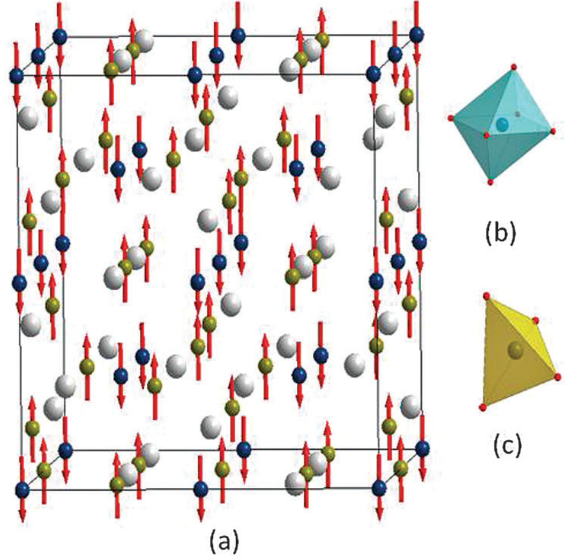
\includegraphics[scale=0.5]{Kap1/LuIG}%
    \caption{(a) Estructura magnética del \ce{Lu3Fe5O12}. Vista de (b) Octaedro
        y (c) tetraedro} \label{fig:luig}
\end{figure}







\chapter{Experimental}

\section{Producción de los Materiales \ce{Lu3Al_{5-x}Fe_{x}O12}}

Los granates de \ce{Lu3Al5O12}:\ce{Ce^{3+}} dopados con \ce{Fe^{3+}} se
prepararon mediante un método de reacción en estado sólido, utilizando
precursores de alta pureza ($\geq$99,99\%) en polvo: \ce{Lu2O3}, \ce{Fe2O3},
\ce{Al(OH)3} y \ce{CeO2}. Los precursores fueron previamente calcinados a
800$^{\circ}$C 
durante 2 horas para eliminar impurezas volátiles, estas mezclas
estequiométricas según la composición granate \ce{Lu3Al_{5-x}Fe_{x}O12} con y x
= 0.0, 0.5, 1.0, 1.5, 2.0, 2.5, 3.0, 3.5, 4.0 y 0.45, se trituraron y prensaron
en pastillas bajo una presión axial de 2.5 MPa y se sinterizaron a
1200$^{\circ}$C  durante 20 horas \cite{Rivera2019}. Además, se utilizó carbón
activo para proporcionar una
atmósfera reductora.

\section{Caracterización}
\subsection{Difracción de Rayos X (DRX)}
Los patrones de difracción de DRX se registraron en un equipo PANalytical
X'Pert PRO-MPD con configuración Bragg-Brentano, usando radiación CuK$\alpha$
($\lambda$ = 1.5406 \r{A}), y un paso de escaneo de 0.02$^o$
en el rango
2$\theta$ 15– 75$^o$. Los datos registrados se utilizaron para análisis
semi-cuantitativo de las fases cristalinas, se utilizó el software X'Pert
HighScore versión 3.0 en conjunto con la base de datos PDF2-2004, para la
determinación de las fases constituyentes. El análisis estructural se realizó
mediante el método de refinamiento de Rietveld, utilizando los paquetes de
software GSAS14 y PCW15. La visualización en 3D de la celda unitaria resultante
se realizó con el paquete de software VESTA16.

\subsection{Reflectancia Difusa y Absorción Óptica}

Los espectros de reflectancia difusa y absorción óptica se obtuvieron usando un
espectrofotómetro Cary 5000 UV-Vis-NIR.

\subsection{Fotoluminiscencia y Eficiencia Cuántica}

Los espectros de fotoluminiscencia a temperatura ambiente y la
fotoluminiscencia dependiente de la temperatura se midieron con un
espectrofotómetro Hitachi F-7000, usando una lámpara Xe de 150 W como fuente de
luz. La eficiencia cuántica externa se midió utilizando una esfera de
integración recubierta de sulfato de bario como estándar de reflectancia en el
mismo espectrofotómetro.

\subsection{Magnetometría de Muestra Vibrante (VSM)}

Las medidas de magnetización fueron
realizadas en un magnetómetro de muestra vibrante VersaLab de Quantum Design, en
función de la temperatura y en función de un campo aplicado para un rango de
(50 a 300) K y para campos magnéticos hasta 30 kOe. Se empleó el método ZFC-FC para
medidas de la magnetización en función de la temperatura.

\subsection{Microscopia Electrónica de Barrido (SEM)}

La morfología de las muestras se observó mediante microscopía electrónica de
barrido (SEM) utilizando el equipo JEOL JSM 6490-LV en 2k, 5k, 10k, 20k y 90k aumentos.
El análisis de espectrometría dispersiva de energía semicuantitativa (EDS) se
realizó utilizando un detector de elementos múltiples. Antes del análisis SEM,
las muestras se recubrieron con grafito para mejorar la conductividad.


\chapter{Análisis Estructural}

\section{Análisis Preliminar}
Los difractogramas obtenidos fueron analizados con el programa
X'Pert$^{\textregistered}$ High Score, en donde, se realizó un análisis preliminar
para determinar la correcta sinterización del granate mediante la comparación
con los registros de la base de datos PDF 2 (2004). A partir de los resultados
obtenidos se determinó que para el material sin sustitución de aluminio (con
x=0.0 \ce{Al5Lu3O12}) hay presencia de la fase cristalina correspondiente al
granate de lutecio aluminio-LUAG (\ce{Al5Lu3O12}) como fase mayoritaria,
identificada con el código de fichero 01-073-1368, que tiene como
características: estructura cúbica y grupo espacial Ia-3d (230). Además, se
encontró presencia de óxido de lutecio (\ce{Lu2O3}) con código 01-086-2475 como
fase minoritaria, de estructura cristalina cubica, grupo espacial Ia-3d (206).
El \ref{AnexoA}-1 muestra el difractograma del \ce{Al5Lu3O12}, en el cual se logran
identificar las fases presentes en el material. Este análisis preliminar se
realizó para todos los difractogramas de DRX obtenidos de cada material del sistema
\ce{Lu3Al_{5-X}Fe_{x}O12}:\ce{Ce^{3+}}, con la finalidad de confirmar la
presencia del granate como fase mayoritaria, las imágenes de los resultados se
presentan en el Anexo \ref{AnexoA}.\\

Los difractogramas obtenidos de cada uno de los materiales del sistema
\ce{Lu3Al_{5-X}Fe_{x}O12}:\ce{Ce^{3+}} (con 0.0 $\leq$ x $<$ 4.5) se agruparon
y se presentan en la Figura \ref{fig:patDRX}. Donde, se pudo determinar
mediante análisis gráfico que se tiene un ligero desplazamiento de las señales
de difracción hacia ángulos inferiores de 2 $\theta$ (ver parte derecha de la
Figura \ref{fig:patDRX}), lo que se relaciona con el aumento de la
concentración de \ce{Fe^{3+}}. Esta variación se atribuye al radio iónico del
\ce{Fe^{3+}} (r = 6.75 \r{A}) que es mayor al radio del \ce{Al^{3+}} (r = 5.85
\r{A}) \cite{Deng2013}. También se observaron señales del difractograma que indican la
presencia de fases cristalinas secundarias para valores de x menores o iguales
a 2.0 (x $\leq$ 2.0) marcadas en la  con (*).

\begin{figure}[h]
    \centering%

    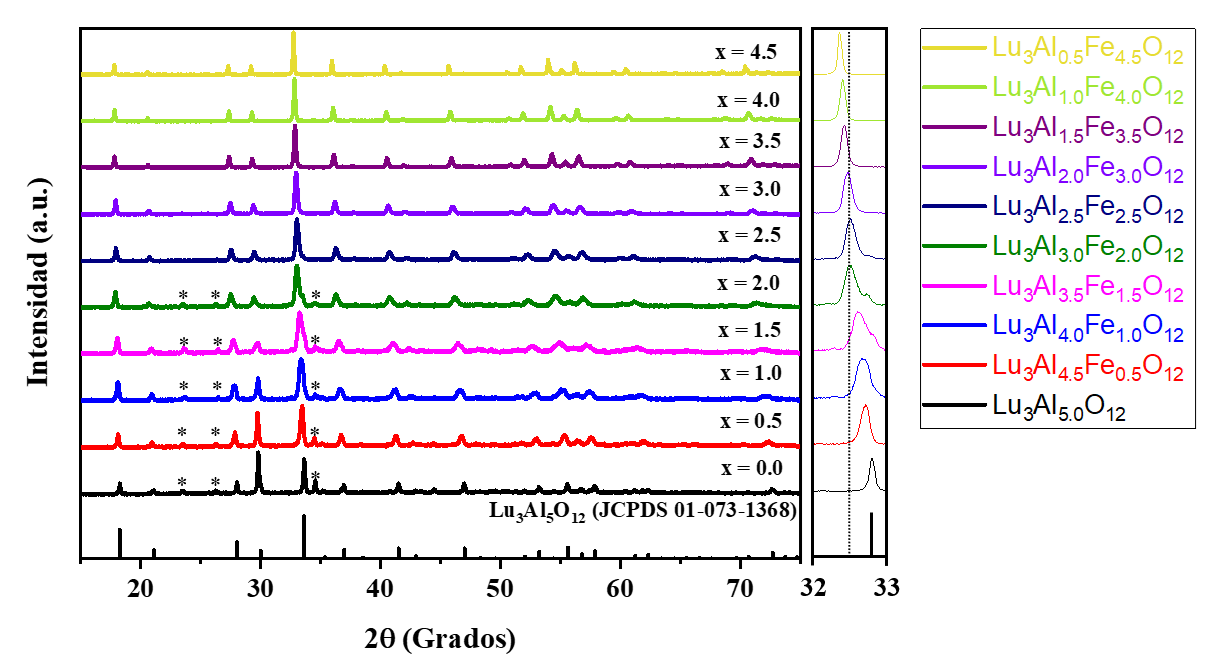
\includegraphics[width=\textwidth]{Kap3/PatronesDRX.png}%
    \caption{Difractogramas DRX de las muestras
    \ce{Lu3Al_{5-X}Fe_{x}O12}:\ce{Ce^{3+}} con 0.0 $\leq$ x $<$4.5; (*)
    Indica las
    señales de difracción asociados a las fases cristalinas secundarias.
    Panel
    derecho:  difractogramas ampliados en el rango de 2$\theta$ 32–33$^o$.}
    \label{fig:patDRX}
\end{figure}

En la Figura \ref{fig:DRXamp} se presenta la región ampliada de 32 a 34 grados
de la señal principal de los difractogramas del sistema
\ce{Lu3Al_{5-X}Fe_{x}O12}:\ce{Ce^{3+}}, en donde, se aprecia mejor la similitud
de cada una de las señales obtenidas y la tendencia del desplazamiento hacia
valores menores de 2$\theta$, también se indica en la figura la relación de los
difractogramas con el aumento de la concentración de \ce{Fe^{3+}} y la
disminución de \ce{Al^{3+}}.

\begin{figure}[h]
    \centering%

    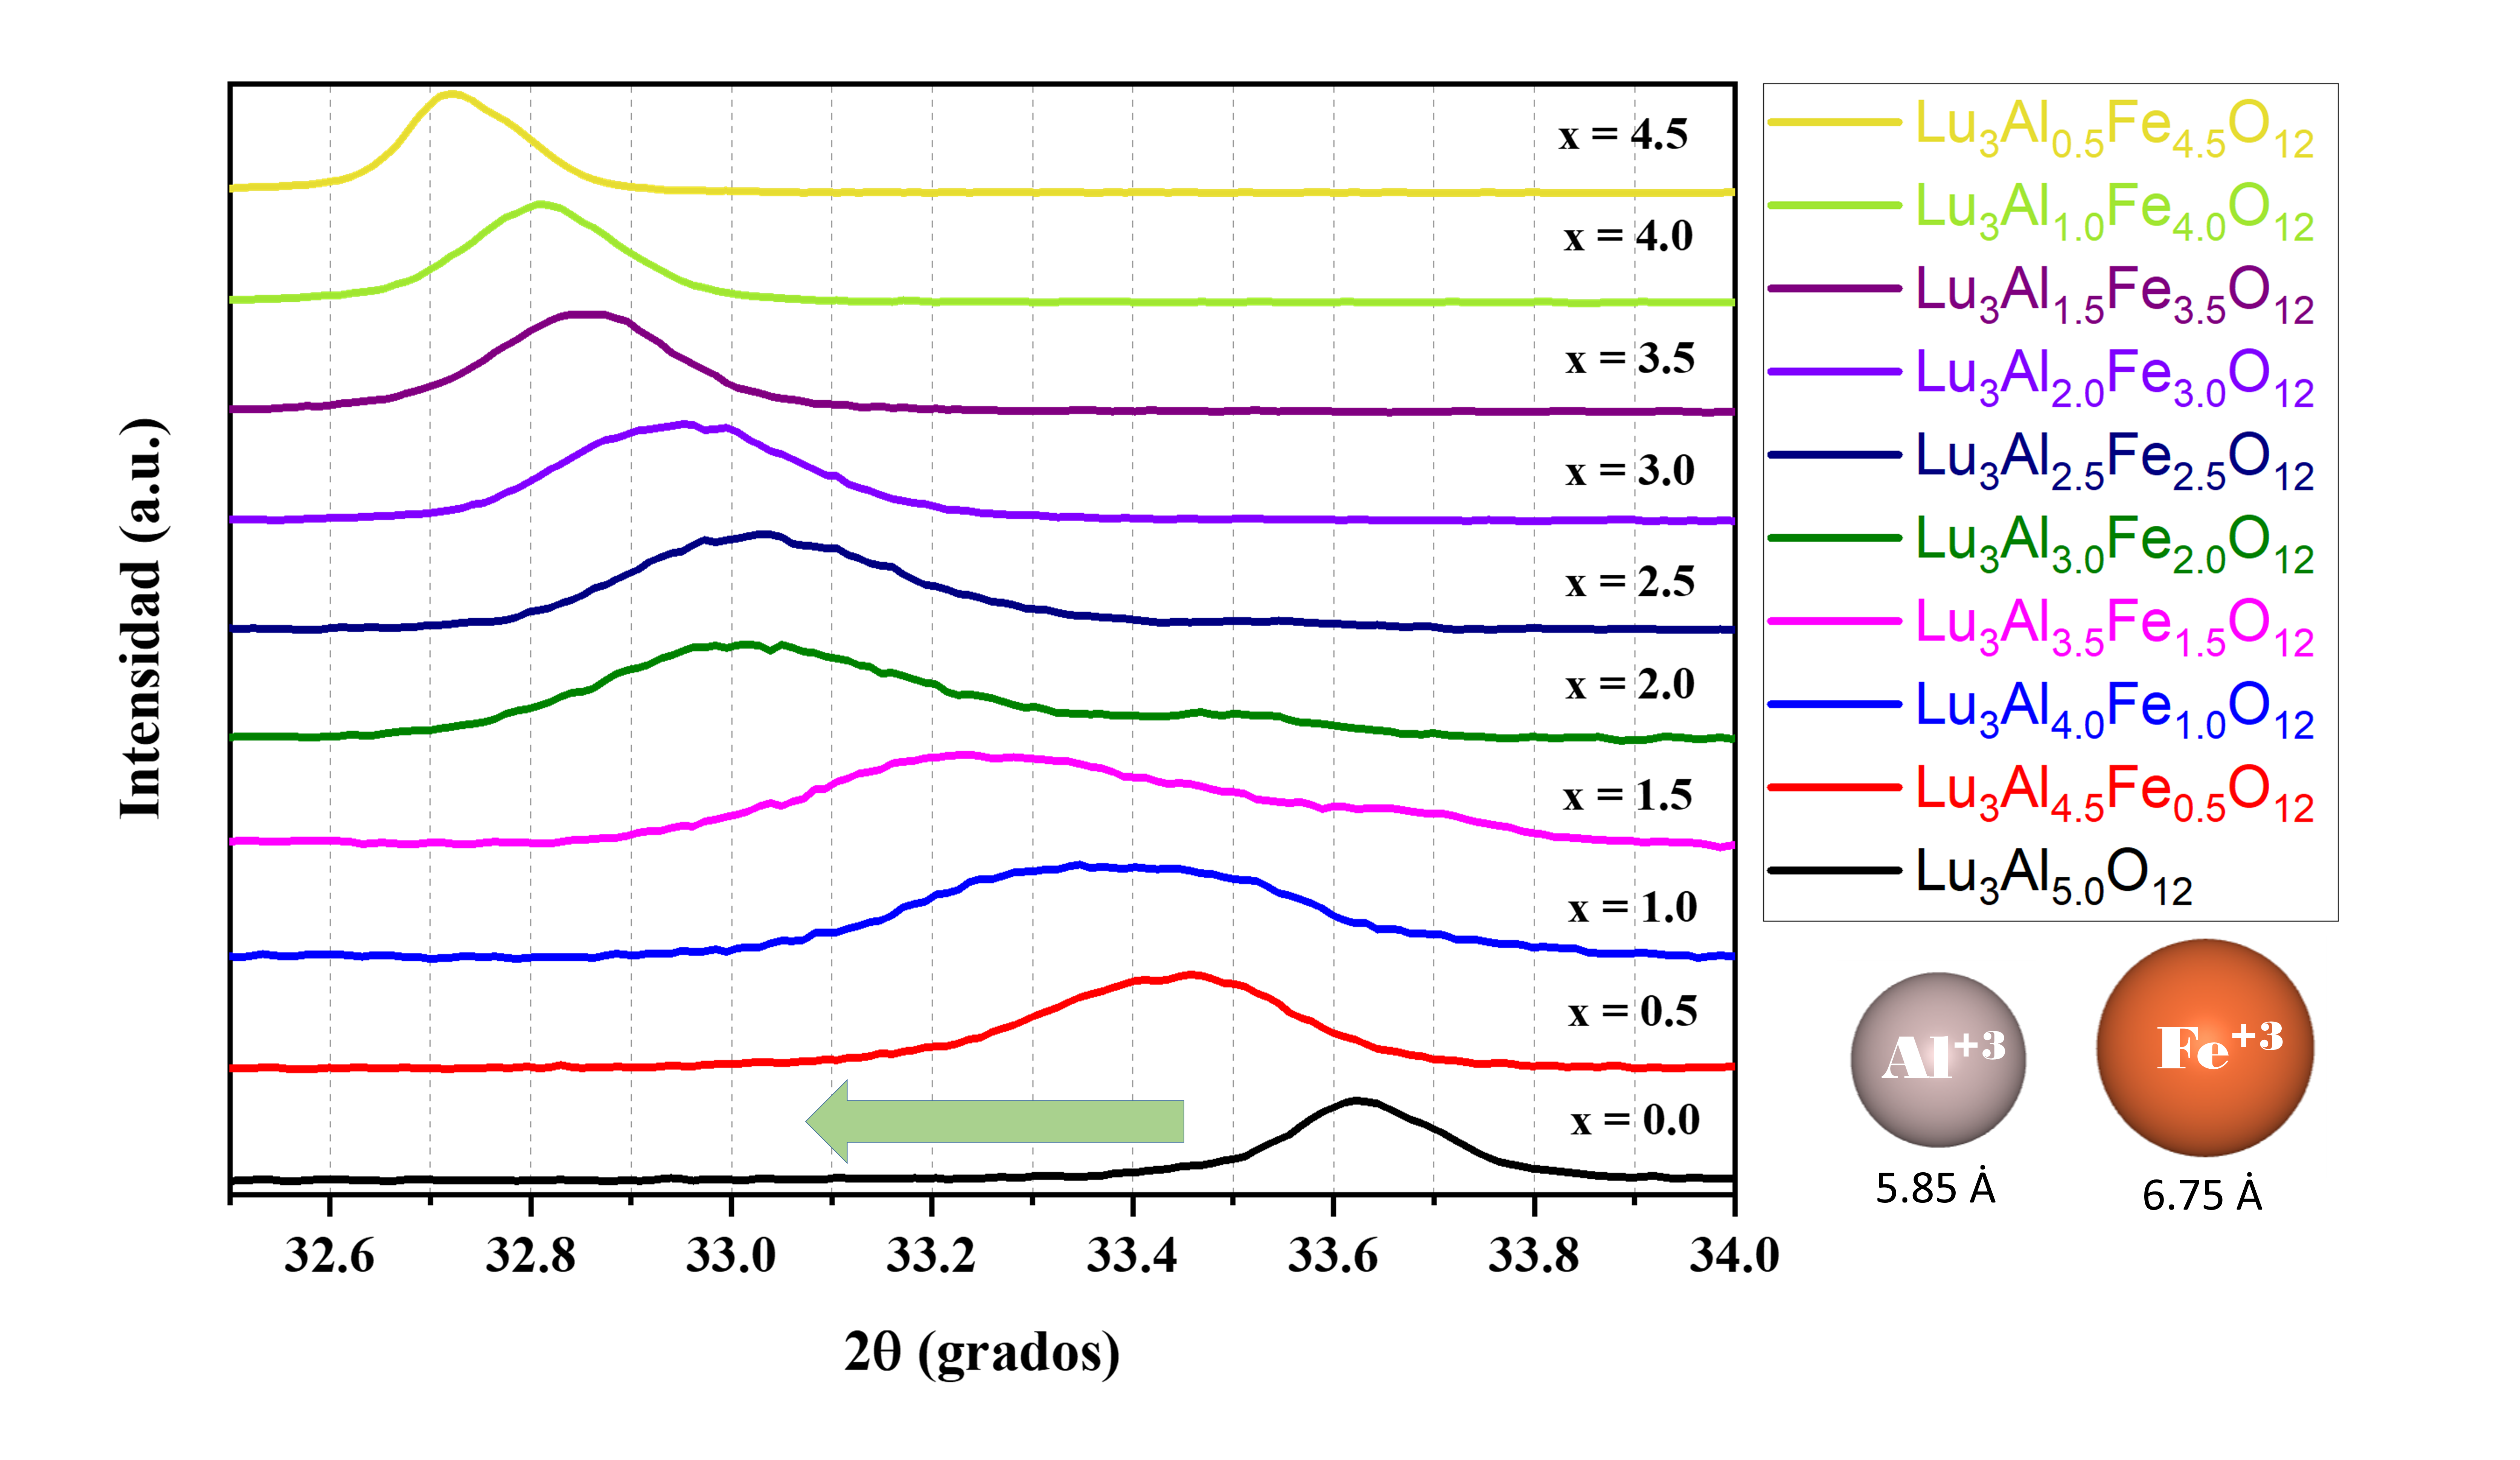
\includegraphics[width=\textwidth]{Kap3/DRXampliado.png}%
    \caption{Región ampliada de la señal principal del sistema de los
    difractogramas DRX de las muestras \ce{Lu3Al_{5-X}Fe_{x}O12}:\ce{Ce^{3+}} en el rango
    de
    2$\theta$ 32–33$^o$} \label{fig:DRXamp}
\end{figure}

\section{Refinamiento Rietveld}

El análisis preliminar realizado con el programa X’Pert\textregistered High
Score permitió
identificar las fases cristalinas presentes en cada material, y sirvió como
punto de partida para proceder con un análisis más detallado mediante el método
de refinamiento Rietveld, apoyado en el uso del software PCW y GSAS, con la
finalidad de determinar los parámetros estructurales y la composición de todas
las muestras producidas para el sistema \ce{Lu3Al_{5-X}Fe_{x}O12}:\ce{Ce^{3+}}
(x= 0.0, 0.5, 1.0, 1.5, 2.0, 2.5, 3.0, 3.5 y 4.5). En la Figura \ref{fig:refi}
se pueden observar los difractogramas refinados para x=0.0 y x=4.5 los demás se
presentan en el Anexo \ref{AnexoB}. Los símbolos (x) representan los difractogramas 
experimentales, la línea roja el difractograma refinado, las barras verticales ($\mid$)
representan las posiciones de Bragg de cada fase identificada, en verde se
muestra el ruido, en azul la diferencia entre el difractograma experimental y el
teórico.\\

\begin{figure}[h]
    \centering%

    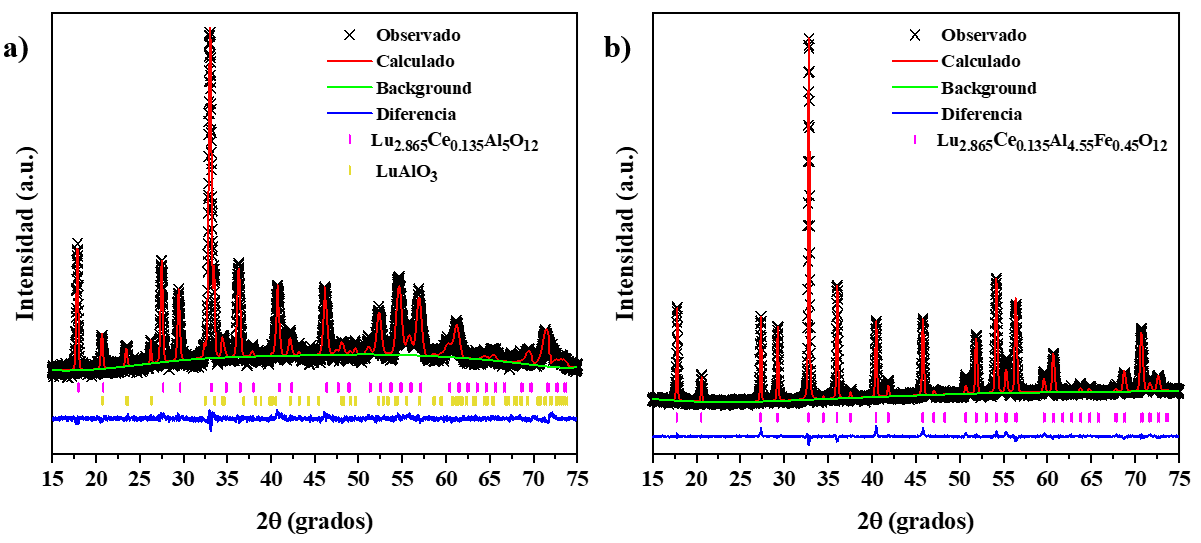
\includegraphics[width=\textwidth]{Kap3/Refinamiento.png}%
    \caption{Difractogramas refinados de DRX para muestras del sistema
    \ce{Lu3Al_{5-X}Fe_{x}O12}, con a) x=0.0, b) x=4.5} \label{fig:refi}
\end{figure}

Los datos estructurales y los factores residuales de cada una de las muestras
se pueden ver en la Tabla 2. Datos estructurales y factores residuales de las
muestras de \ce{Lu3Al_{5-X}Fe_{x}O12}:\ce{Ce^{3+}}, donde se determinó la
presencia como fase cristalina principal el granate \ce{Lu3Al5O12} (JCPDS
01-073-1368) con estructura cubica y grupo espacial l3d (230). Para
concentraciones bajas de \ce{Fe^{3+}} (0.0 $\leq$ x $\leq$ 4.5) se identificó
como
fase secundaria el \ce{LuAlO3} (JCPDS 00-024-0690). Sin embargo, se obtuvieron
materiales de fase única partir de valores de x mayores o iguales a 2.5 (x
$\geq$ 2.5), lo que se le atribuye a la menor temperatura de fusión del
precursor de \ce{Fe^{3+}} comparada con la del \ce{Al^{3+}}, la cual favoreció
la difusión iónica y la formación la estructura del granate.\\

En la Figura \ref{fig:para} a) se presenta la relación entre el parámetro de
red de la
celda unidad y el aumento de la concentración \ce{Fe^{3+}}, donde se tiene una
tendencia lineal hacia la expansión de la celda unidad, que se puede relacionar
con el desplazamiento de las señales de DRX y también confirma la sustitución
de \ce{Fe^{3+}} por \ce{Al^{3+}} en la estructura del granate, al relacionarse
con la Ley de Vegard, que indica que el parámetro de red de la estructura
cristalina
resultante es una media ponderada de los constituyentes \cite{Kempter1966,King1921}. En la Figura
\ref{fig:para}
b) podemos observar representación en tres dimensiones (3D) de la celda unidad
siguiendo
los datos obtenidos del refinamiento para el sistema granate
\ce{Lu3Al_{5-X}Fe_{x}O12}:\ce{Ce^{3+}}, donde, los átomos de Lu y Ce ocupan los
sitios 24(c) formando un dodecaedro, los átomos de Al y Fe ocupan los sitios
24(d) formando un tetraedro, y los sitios 16(a) formando un octaedro.\\

\begin{figure}[h]
    \centering%

    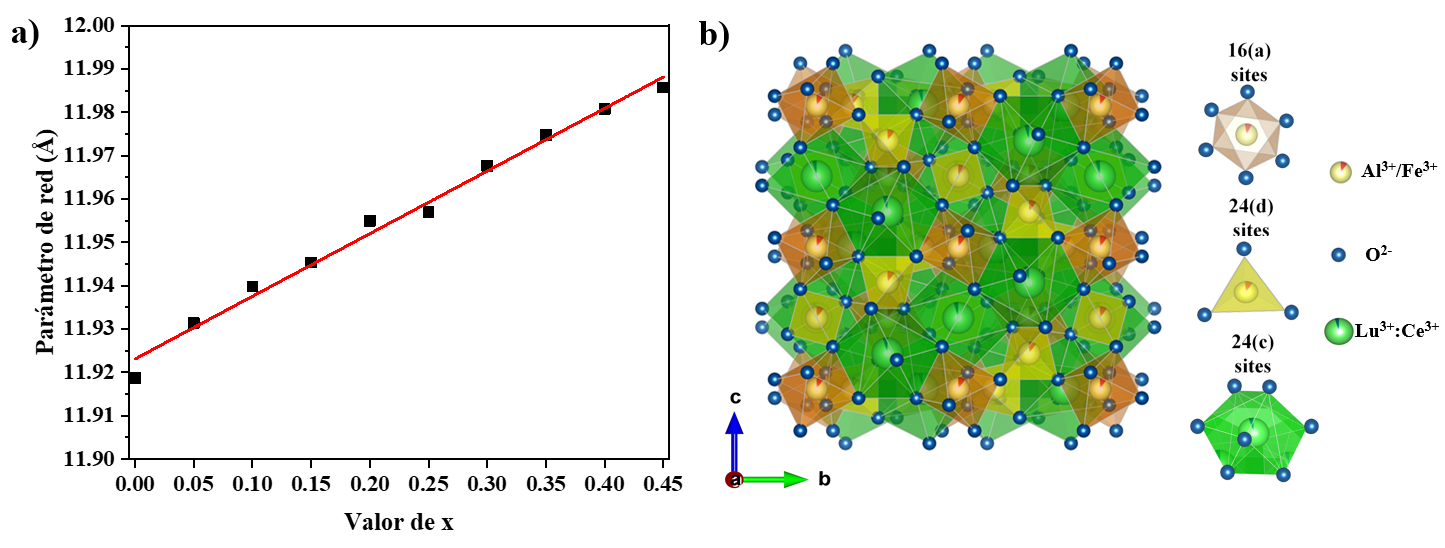
\includegraphics[width=\textwidth]{Kap3/ParametroRed.png}%
    \caption{Parámetro de red a como función de la concentración de
    \ce{Fe^{3+}}
    (valor de x) y una vista en 3D de la celda unitaria del sistema granate
    \ce{Lu3Al_{5-X}Fe_{x}O12}:\ce{Ce^{3+}}}
    \label{fig:para}
\end{figure}

\section{Espectroscopia del Infrarrojo Cercano}

Se registraron espectros de absorción en la región de infrarrojos cercanos
(NIR) para verificar la modificación de las bandas electrónicas y vibratorias,
generadas por la inserción \ce{Fe^{3+}} en la estructura del granate. En La
Figura \ref{fig:nir} se presentan los espectros NIR para las muestras del
sistema
\ce{Lu3Al_{5-X}Fe_{x}O12}:\ce{Ce^{3+}} (x = 0.0 y 4.5).\\

\begin{figure}[h]
    \centering%

    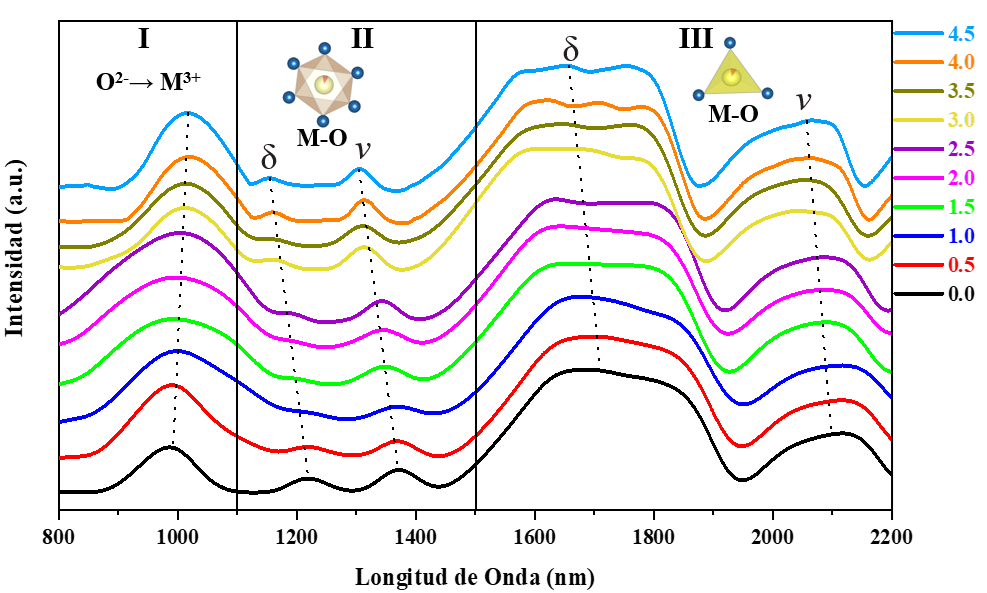
\includegraphics[width=\textwidth]{Kap3/NIR.png}%
    \caption{Espectros de absorción en la región NIR para las muestras
    \ce{Lu3Al_{5-X}Fe_{x}O12}:\ce{Ce^{3+}} (0.0 $\leq$ x $\leq$ 4.5)}
    \label{fig:nir}
\end{figure}

Los espectros se pueden separar en tres regiones principales, a las que se
atribuyen: absorción electrónica debido a la transferencia de carga
oxígeno-metal (I), y absorciones vibratorias atribuidas al estiramiento ($\upsilon$ ) y
flexión ($\sigma$) de la unión metal-oxígeno en configuraciones octaedro (II) y
tetraedro (III). Las bandas asociadas a la transferencia de carga oxígeno-metal
se encuentran en el rango espectral 800-1100 nm \cite{Rossman2019}. Al aumentar la concentración
\ce{Fe^{3+}}, la banda exhibió un desplazamiento hacia longitudes de onda más largas
(disminución de la energía), esto se atribuye a las variaciones en los
poliedros locales y la mezcla de estados excitados \cite{Krambrock2013}. Los cationes trivalentes
exhiben un mayor radio iónico efectivo cuando
están en configuración octaédrica, y existe una mayor repulsión electrostática
de los seis átomos de oxígeno que los rodean. Entonces, las bandas atribuidas a
la absorción vibracional de la configuración octaédrica se ubican en longitudes
de onda más cortas que las de la configuración tetraédrica \cite{Rossman2019}. La longitud de
onda de las absorciones vibratorias es proporcional al poder de polarización
del catión en una configuración octaédrica o tetraédrica. El catión \ce{Fe^{3+}} tiene
un poder de polarización menor (4.76) que el \ce{Al^{3+}} (5.66) \cite{Bishop2019}, por lo tanto, una
mayor concentración de \ce{Fe^{3+}} en los granates condujo a una disminución
progresiva en la longitud de onda de las absorciones vibratorias.                                                                                                                                                                     
\chapter{Caracterización Óptica}
\section{Reflectancia Difusa}

En la Figura \ref{fig:reflectancia} se puede observar los espectros de
reflectancia difusa de las muestras \ce{Lu3Al_{5-X}Fe_{x}O12}:\ce{Ce^{3+}}.
Donde el material con x = 0.0 mostró una reflectancia intensa en la región
visible (300-800) nm, que disminuye en la región ultravioleta (200-300) nm.  El
aumento de la
concentración de \ce{Fe^{3+}} generó una disminución progresiva de la
reflectancia en
la región visible, así como un fenómeno de desplazamiento del rojo, esto se
puede atribuir a la reducción de energía de banda \cite{Zhou2017}.\\

\begin{figure}[h]
    \centering%

    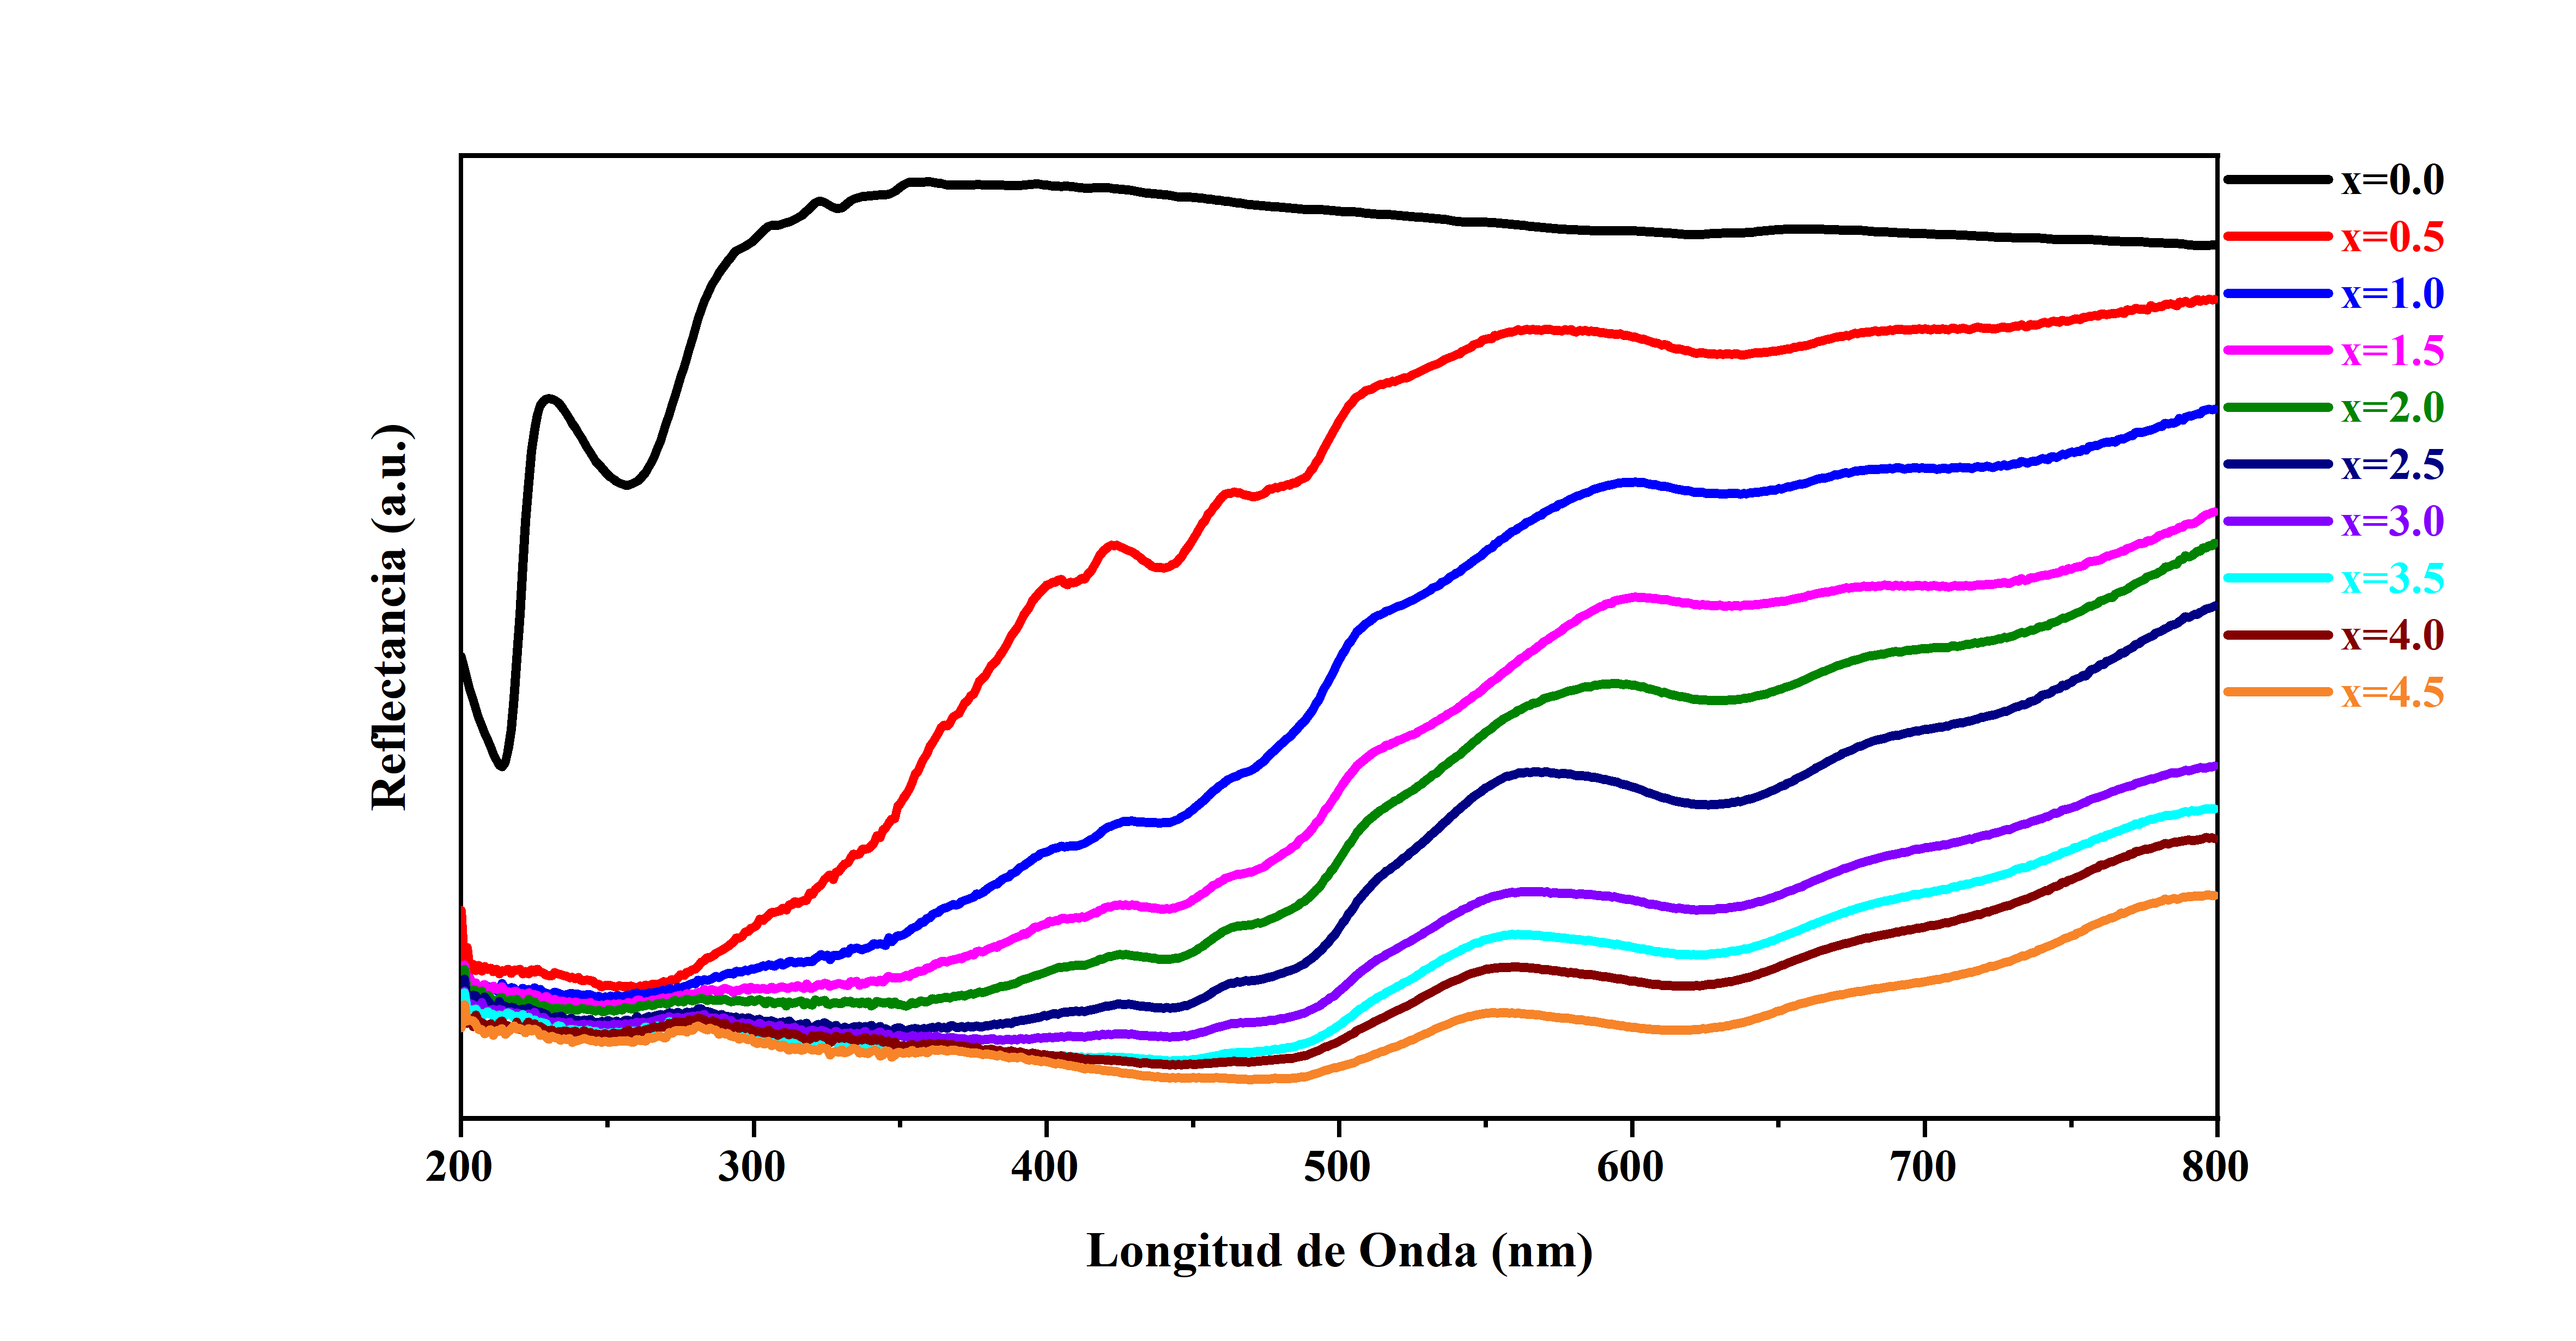
\includegraphics[width=\textwidth]{Kap4/ReflectanciaDifusa.png}%
    \caption{Espectros de reflectancia difusa de las muestras de
    \ce{Lu3Al_{5-X}Fe_{x}O12}:\ce{Ce^{3+}}} \label{fig:reflectancia}
\end{figure}

Los valores de la energía banda prohibida (\ce{E_{g}}) se estimaron mediante
extrapolación
lineal de los diagramas de Tauc \cite{Deng2013}, que se determinaron mediante
la Ecuación \ref{eqn:eq1} \cite{Mott1970}.\\

\begin{equation}
    [(F(R) h \nu)^{n}=A(h \nu - E_{g})]
    \label{eqn:eq1}
\end{equation}

donde,$A$ es una constante proporcional, $h \nu$ es la energía del fotón, $n$
es el coeficiente que denota la naturaleza de la transición ($n=2$ para
transiciones directas permitidas, $n=2/3$ para transiciones directas
prohibidas, $n=1/2$ para transiciones indirectas permitidas y $n=1/3$ para
transiciones indirectas prohibidas) \cite{Mott1970}, y $F(R)$ es la función
Kubeka-Munk
(ver Ecuación \ref{eqn:eq2}) \cite{Simmons1975}, en el que $R$ es la
reflectancia:

\begin{equation}
    F(R)=\frac{(1-R)^2}{2R}
    \label{eqn:eq2}
\end{equation}

En la Figura \ref{fig:tauc} (a) y (b) se puede observar las gráficas de Tauc para
las
muestras del sistema \ce{Lu3Al_{5-X}Fe_{x}O12}:\ce{Ce^{3+}}. Los datos
experimentales se
ajustaron bien con $n = 2$, lo que indica la existencia de transiciones
directas
permitidas. La $E_{g}$ disminuyó progresivamente conforme al aumento en la
concentración \ce{Fe^{3+}} (ver Figura \ref{fig:tauc} c), lo que se relaciona
con el
incremento del
valor para el parámetro de red \cite{J.C.Inkson2012}. En un semiconductor
cúbico, la $E_{g}$
disminuye proporcionalmente al cuadrado del parámetro de red \cite{Dalven1973},
esto se
puede atribuir a la energía de enlace de la disminución de valencia al aumentar
la distancia interatómica, requiriendo menos energía para liberar los
electrones de la banda de conducción.\\

\begin{figure}[H]
    \centering%

    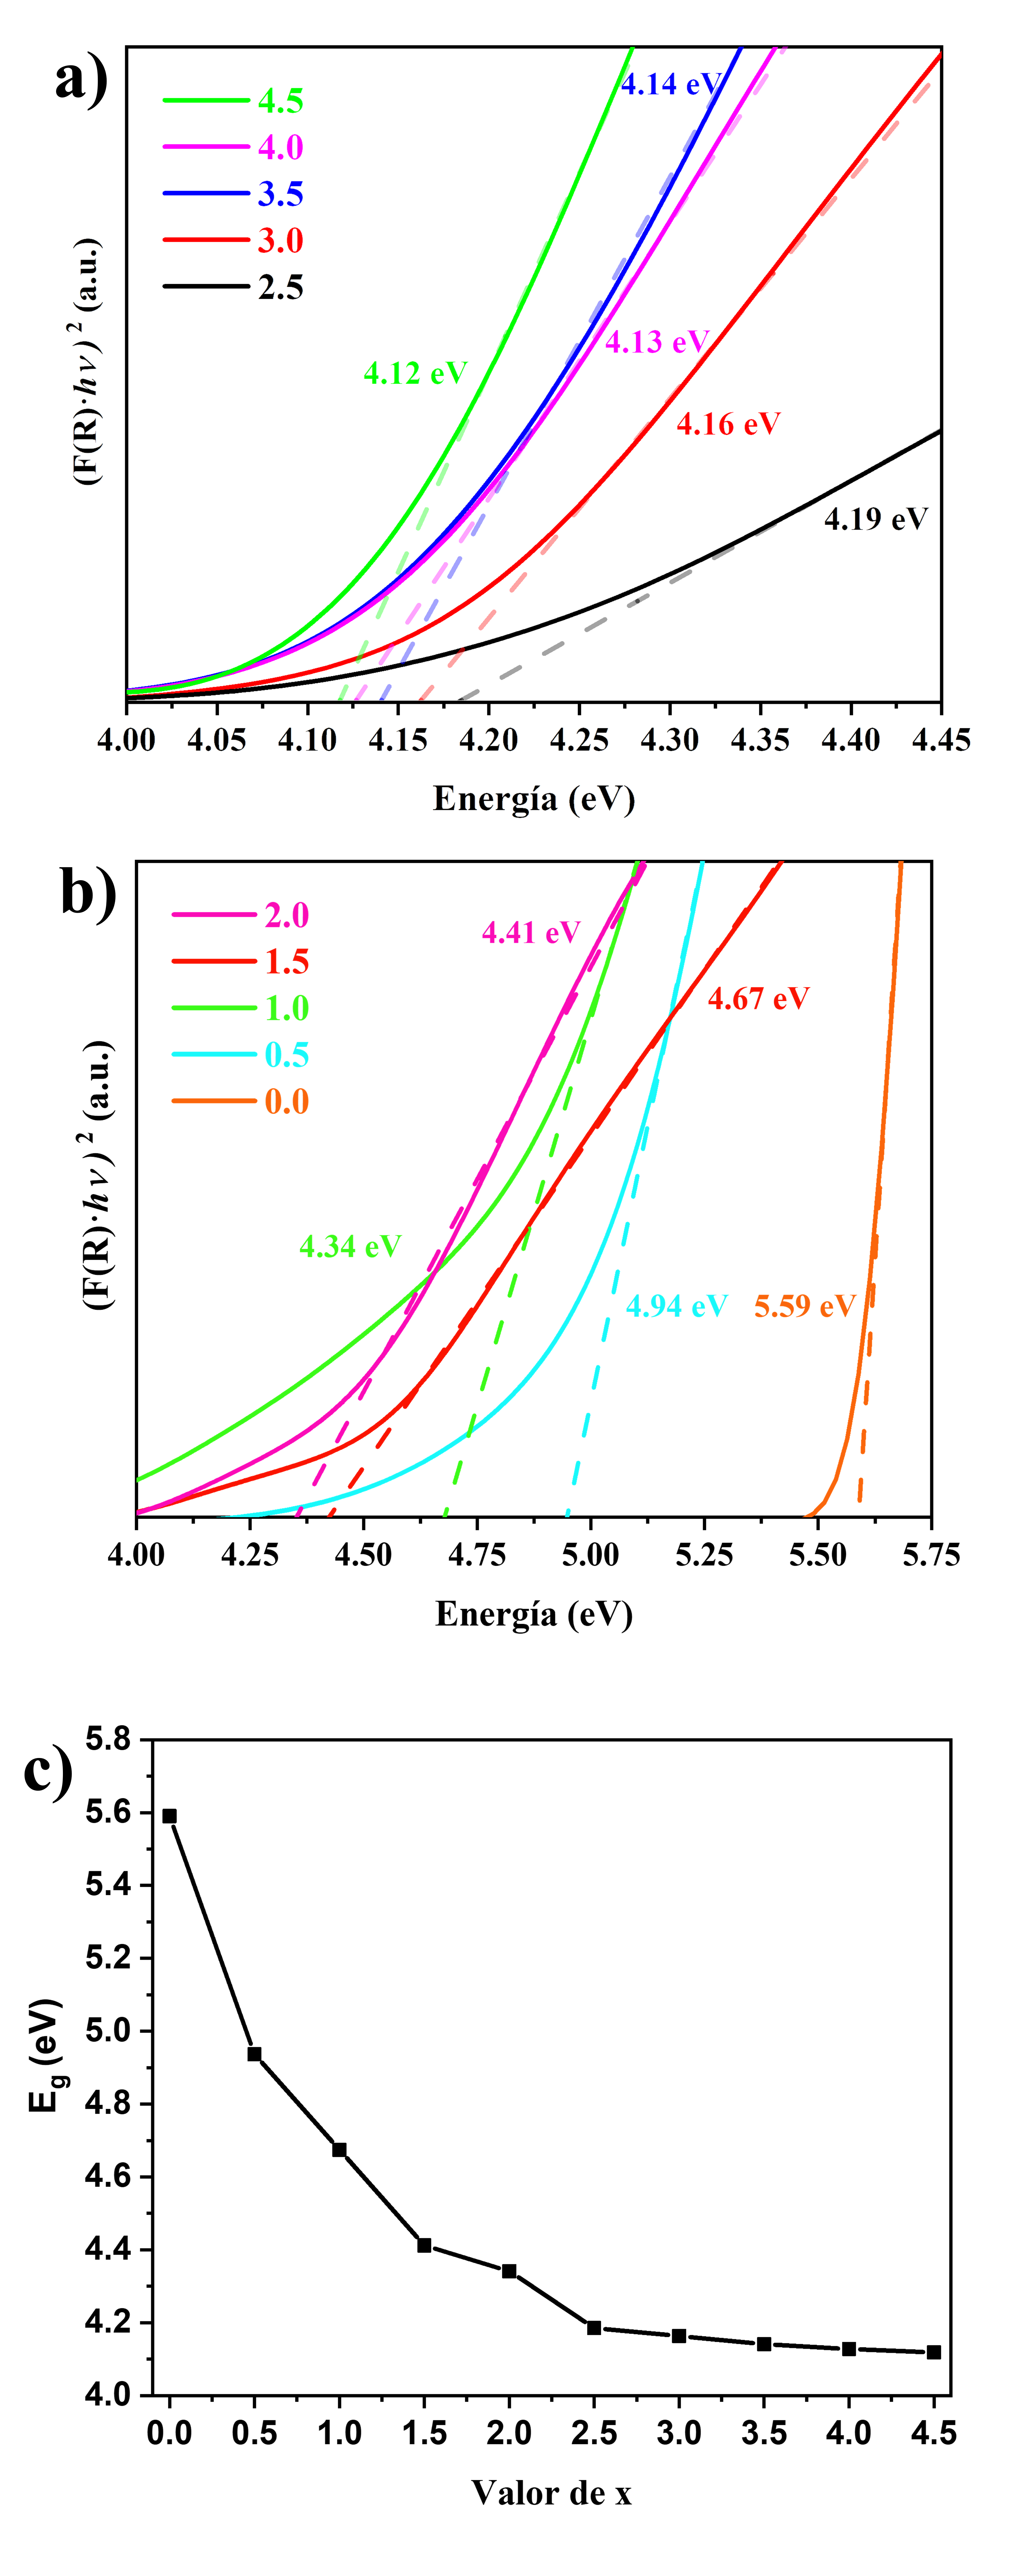
\includegraphics[width=0.45\textwidth]{Kap4/Tauc2.png}%
    \caption{a) y b) Gráficas de Tauc de las muestras del sistema
    \ce{Lu3Al_{5-X}Fe_{x}O12}:\ce{Ce^{3+}} y c) $E_g$ en función de la
    concentración de \ce{Fe^{3+}}}\label{fig:tauc}
\end{figure}

\section{Espectro de Absorción}

En la estructura granate, los cationes \ce{Ce^{3+}} se encuentran en los sitios
dodecaédricos, generando un estado doblemente degenerado ($^{2}E_{g}$) y un
estado
triplemente degenerado ($^{2}T_{g}$), con un campo cristalino habitual que se
divide
($\varepsilon_{0}$) entre el nivel más bajo ($5d_{1}$) y el nivel más alto
($5d_5$). Sin embargo, los
niveles de $5d_1$ y $5d_2$ del estado $^2E_g$ se dividen más que los de
coordinación
cúbica u octaédrica, lo que lleva a una división adicional del campo cristalino
\cite{Dorenbos2003}
($\Delta_{1-2}$). Como resultado, todas las muestras exhibieron tres bandas de
adsorción en la región UV-Vis (Figura \ref{fig:abso}). Las bandas ubicadas en
el rango
espectral de (200-230) nm son atribuibles a las transiciones superpuestas $4f$
$(2F_{5/2}) \rightarrow ^2T_g(^5d_{5,4,3})$ y las bandas restantes ubicadas
alrededor de (350 y 450)
nm corresponden a las transiciones $4f(^2F_{5/2}) \rightarrow ^2E_g (^5d_2)$ y
    $4f(^2F_{5/2}) \rightarrow ^2E_g
    (5d_1)$, respectivamente \cite{Ueda2019}.\\

\begin{figure}[H]
    \centering%

    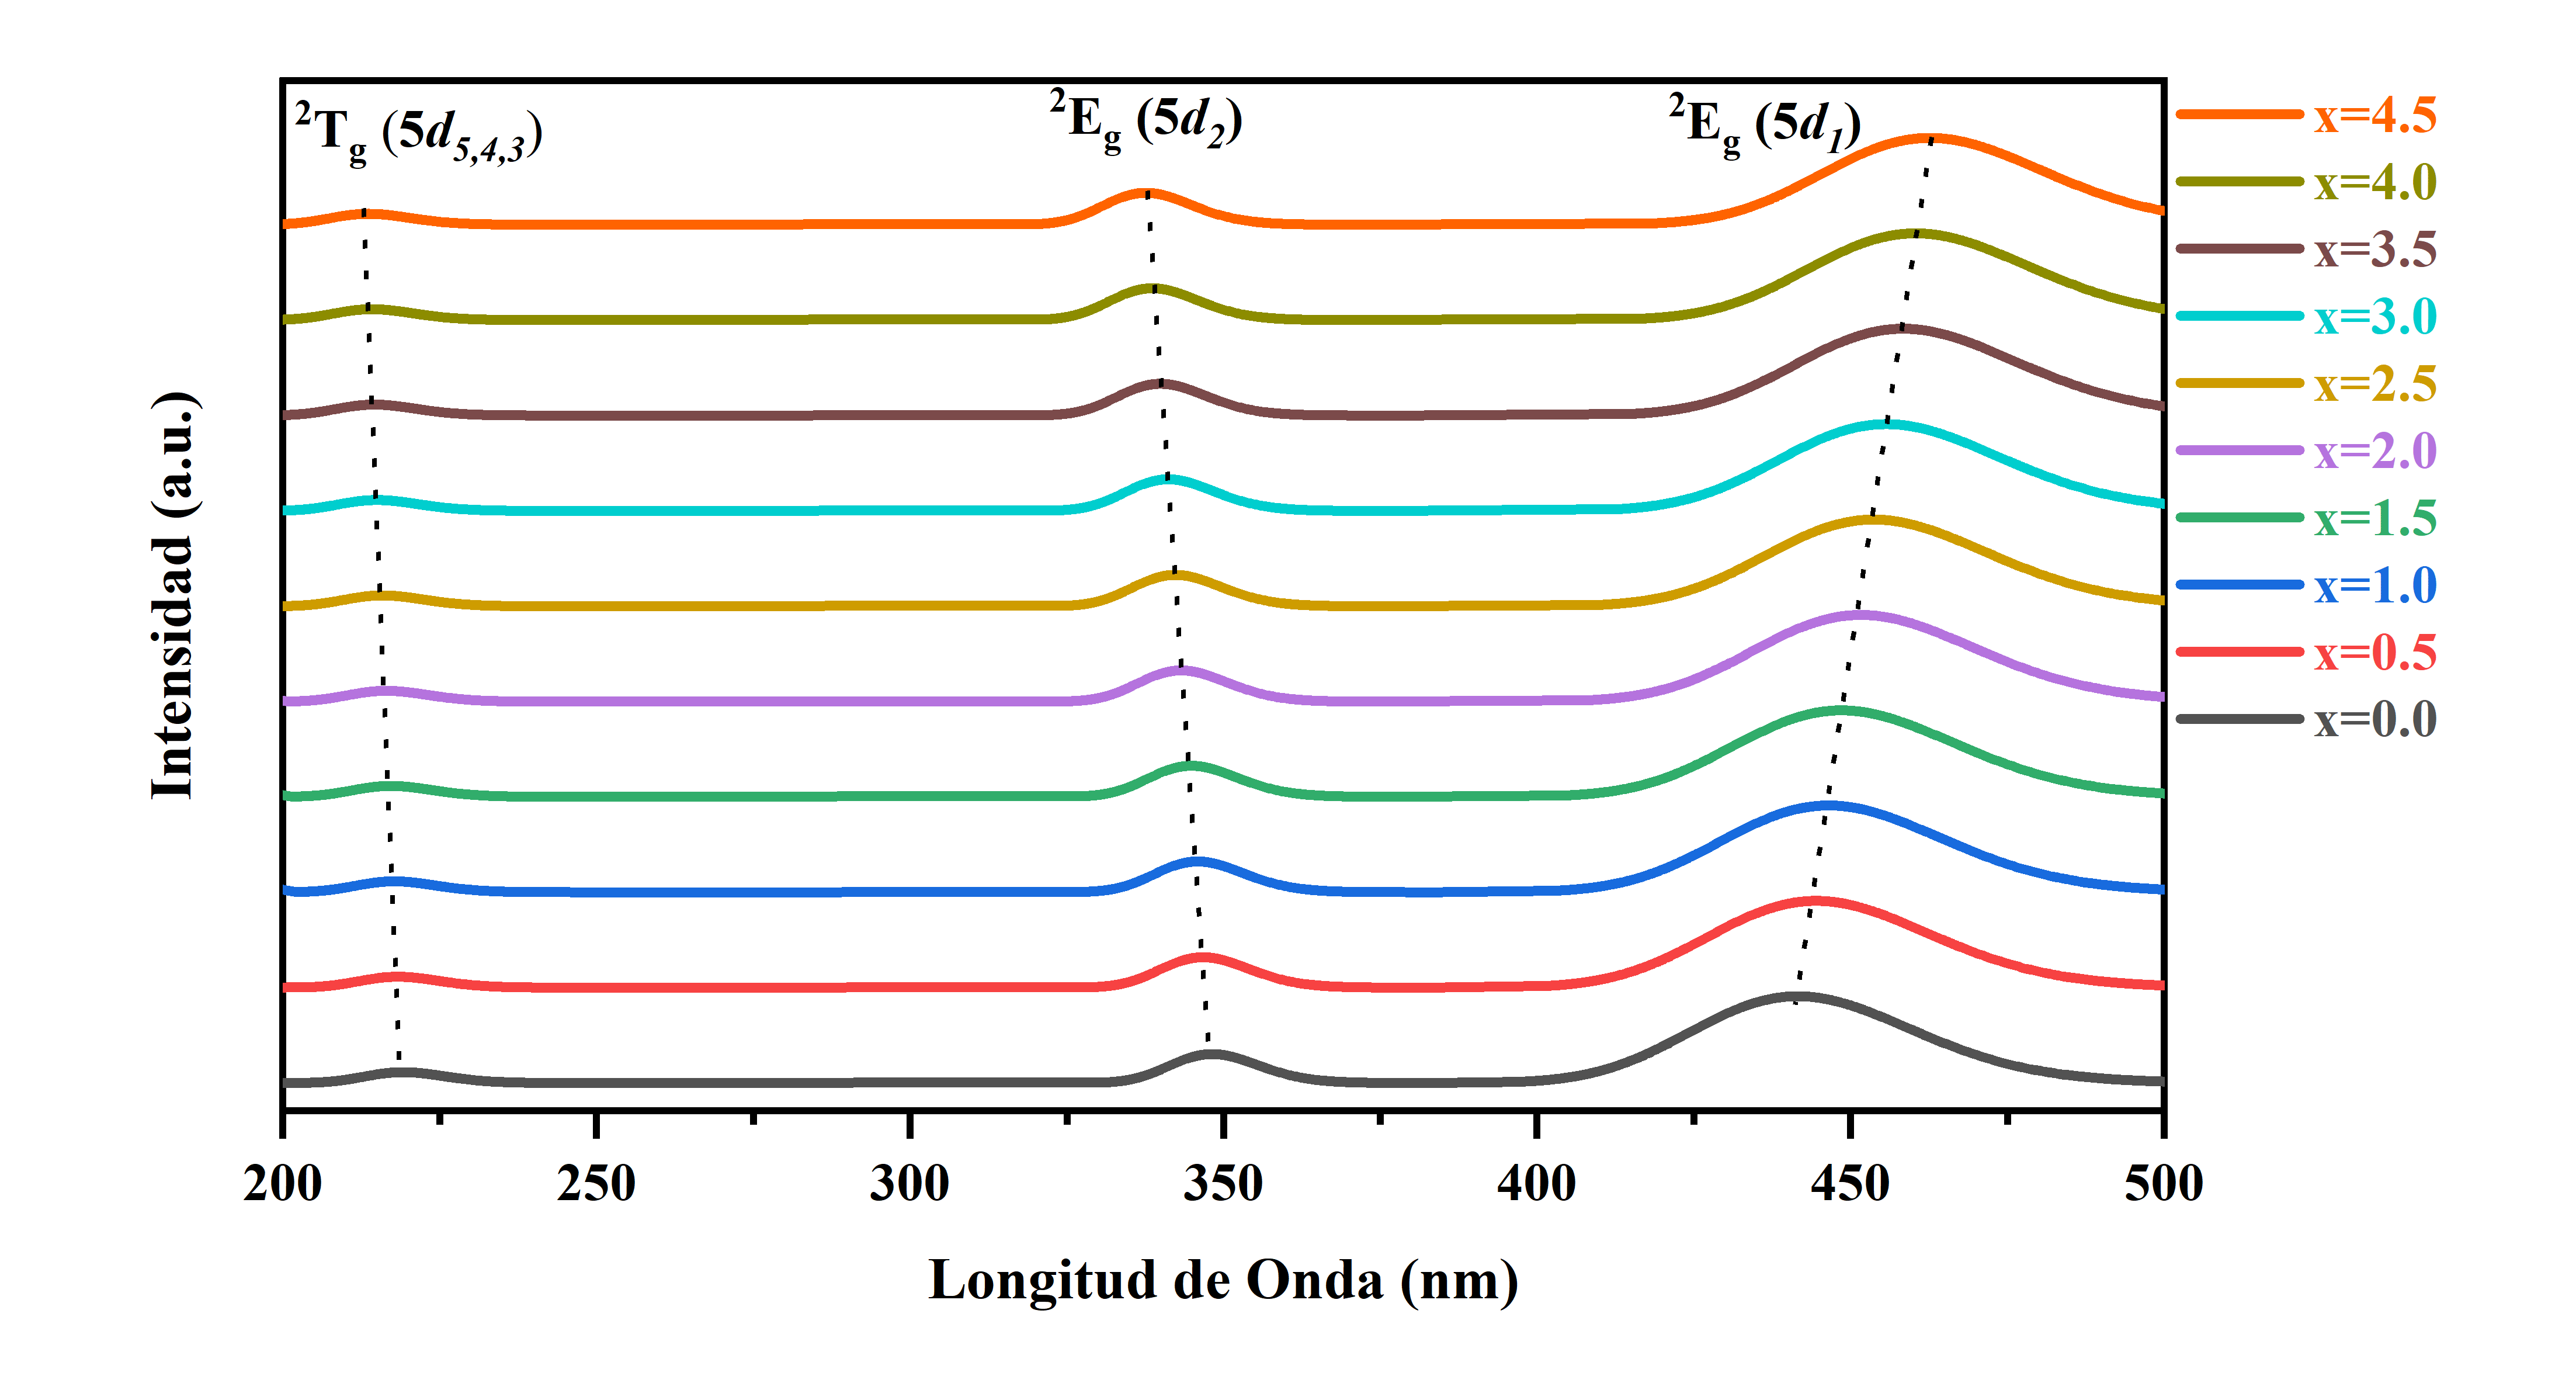
\includegraphics[width=\textwidth]{Kap4/Absorcion.png}%
    \caption{Espectros de absorción en la región UV-Vis para las muestras de
    \ce{Lu3Al_{5-X}Fe_{x}O12}:\ce{Ce^{3+}} (0.0 $\leq x \leq$
    4.5)}\label{fig:abso}
\end{figure}

Al aumentar la concentración de \ce{Fe^{3+}} en las muestras, las bandas
asociadas a
las transiciones $4f(^2F_{5/2}) \rightarrow ^2T_g (5d_{5,4,3})$ y
$4f(^2F_{5/2}) \rightarrow ^2E_g (5d_2)$ mostraron
un desplazamiento hacia longitudes de onda más corta (desplazamiento hacia el
azul). Por el contrario, la banda asociada a la transición $4f(^2F_{5/2})
    \rightarrow ^2E_g(5d_1)$ mostró un desplazamiento hacia longitudes de onda
más
largas
(desplazamiento hacia el rojo). La energía de los niveles $5d$ es sensible
a
las variaciones estructurales \cite{Xu2014}, y la energía de separación del
campo
cristalino \cite{Dorenbos2003}. El dopaje con \ce{Fe^{3+}} generó la
intensificación de las
energías
($\varepsilon_{0}$) y $\Delta_{1-2}$, aumentando la energía de las
$^2T_g(5d_{5,4,3})$ y los niveles $2E_g(5d_2)$,
pero disminuyendo la energía del nivel $2E_g(5d_1)$. La longitud de onda de las
bandas de absorción y los valores de las energías ($\varepsilon_{0}$) y
$\Delta_{1-2}$ se presentan en la
Tabla \ref{tab:longitudOnda}. Con base en cálculos teóricos, realizados por
Chen et al
\cite{Chen2015a}. Se
estableció que la inserción de cationes más grandes en la estructura del
granate genera un fuerte efecto compresivo, lo que lleva a la generación de
orbitales moleculares híbridos a partir del orbitales d del metal y el orbital
2p del oxígeno.\\

\begin{table}[h]
    \caption{Longitud de onda (nm) y energía (eV) de los estados excitados para
    \ce{Ce^{3+}} en materiales \ce{Lu3Al_{5-X}Fe_{x}O12}:\ce{Ce^{3+}}, y
    energías
    de separación de campo cristalino $\varepsilon_0$ y $\Delta_{1-2}$}
    \label{tab:longitudOnda}
    \resizebox{\textwidth}{!}{%
        \begin{tabular}{@{}llllllll@{}}
            \toprule
                                                  & \multicolumn{5}{l}{Banda de
                Absorción nm (eV)}

                                                  &
                                                  &
            \\ \cmidrule(lr){2-6}
            \multirow{-2}{*}{Valor de X}          & 5d5
                                                  & 5d4
                                                  & 5d3
                                                  & 5d2
                                                  & 5d1
                                                  &
            \multirow{-2}{*}{$\varepsilon (eV)$}                   & \multirow{-2}{*}{$\Delta_{1-2}$
                (eV)}
            \\ \midrule
            0.0                                   & 209 (5.93)
                                                  & 219
            (5.66)                             & 228 (5.44)
                                                  & 348
            (3.56)                             & 442 (2.81)
                                                  &
            2.63                                  & 0.75
            \\
            0.5                                   & 208
            (5.95)                             &
            218 (5.68) & 227
            (5.46)                             &
            347 (3.58) & 444
            (2.79)                             &
            2.67          &
            0.79
            \\
            1.0                                   & 208 (5.97)
                                                  & 218
            (5.69)                             & 227 (5.47)
                                                  & 346
            (3.59)                             & 446 (2.78)
                                                  &
            2.69                                  & 0.81
            \\
            1.5                                   & 207
            (5.99)                             &
            217 (5.71) & 226
            (5.48)                             &
            345 (3.60) & 448
            (2.76)                             &
            2.72          &
            0.83
            \\
            2.0                                   & 206 (6.01)
                                                  & 216
            (5.73)                             & 225 (5.50)
                                                  & 343
            (3.61)                             & 452 (2.75)
                                                  &
            2.75                                  & 0.87
            \\
            2.5                                   & 206
            (6.02)                             &
            216 (5.74) & 225
            (5.51)                             &
            342 (3.62) & 454
            (2.73)                             &
            2.78          &
            0.89
            \\
            3.0                                   & 205 (6.05)
                                                  & 215
            (5.77)                             & 224 (5.53)
                                                  & 341
            (3.63)                             & 456 (2.72)
                                                  &
            2.81                                  & 0.91
            \\
            3.5                                   & 205
            (6.06)                             &
            215 (5.78) & 224
            (5.54)                             &
            340 (3.65) & 458
            (2.71)                             &
            2.84          &
            0.94
            \\
            4.0                                   & 204 (6.07)
                                                  & 214
            (5.79)                             & 223 (5.56)
                                                  & 339
            (3.66)                             & 460 (2.69)
                                                  &
            2.86                                  & 0.97
            \\
            4.5                                   & 204
            (6.09)                             &
            214 (5.80) & 223
            (5.57)                             &
            338 (3.67) & 462
            (2.68)                             &
            2.89          &
            0.99
            \\ \bottomrule
        \end{tabular}%
    }
\end{table}

Esta hibridación de orbitales conduce a una fuerte disminución de la energía de
banda prohibida ($E_g$) debido a la expansión de la banda de conducción, la
reducción de la masa efectiva del electrón y una intensificación de la energía
del campo cristalino \cite{Chen2015a}.\\

\section{Fotoluminisencia}

Las muestras de \ce{Lu3Al_{5-X}Fe_{x}O12}:\ce{Ce^{3+}} con x $\geq $ 1.5
exhibieron fotoluminiscencia
bajo irradiación azul (436 nm), exhibiendo bandas asimétricas en el rango
espectral de (450–650) nm (Figura \ref{fig:foto} a). Las bandas de emisión fueron
decombolucionadas en dos perfiles gaussianos (como se muestra en el inserto de
la Figura \ref{fig:foto} a. las cuales son atribuidas a transiciones desde el
nivel más
bajo de $^2E_g(5d_1)$ a los estados fundamentales $^2F_{5/2}$ y $^2F_{7/2}$,
respectivamente \cite{Yu2014}. Los anchos de banda obtenidos fueron
considerablemente amplios debido
al
fuerte acoplamiento fonónico \cite{Ueda2019}, e indican efectos de campo
cristalino en los
estados excitados del \ce{Ce^{3+}} \cite{Miniscalco1978}. Además, la inserción
de \ce{Fe^{3+}}
provocó un
desplazamiento de las bandas de emisión, lo que sugiere que las bandas se deben
a una transferencia de carga no relajada entre los cationes \ce{Ce^{3+}}
\cite{Zhang2014}.\\

\begin{figure}[h]
    \centering%

    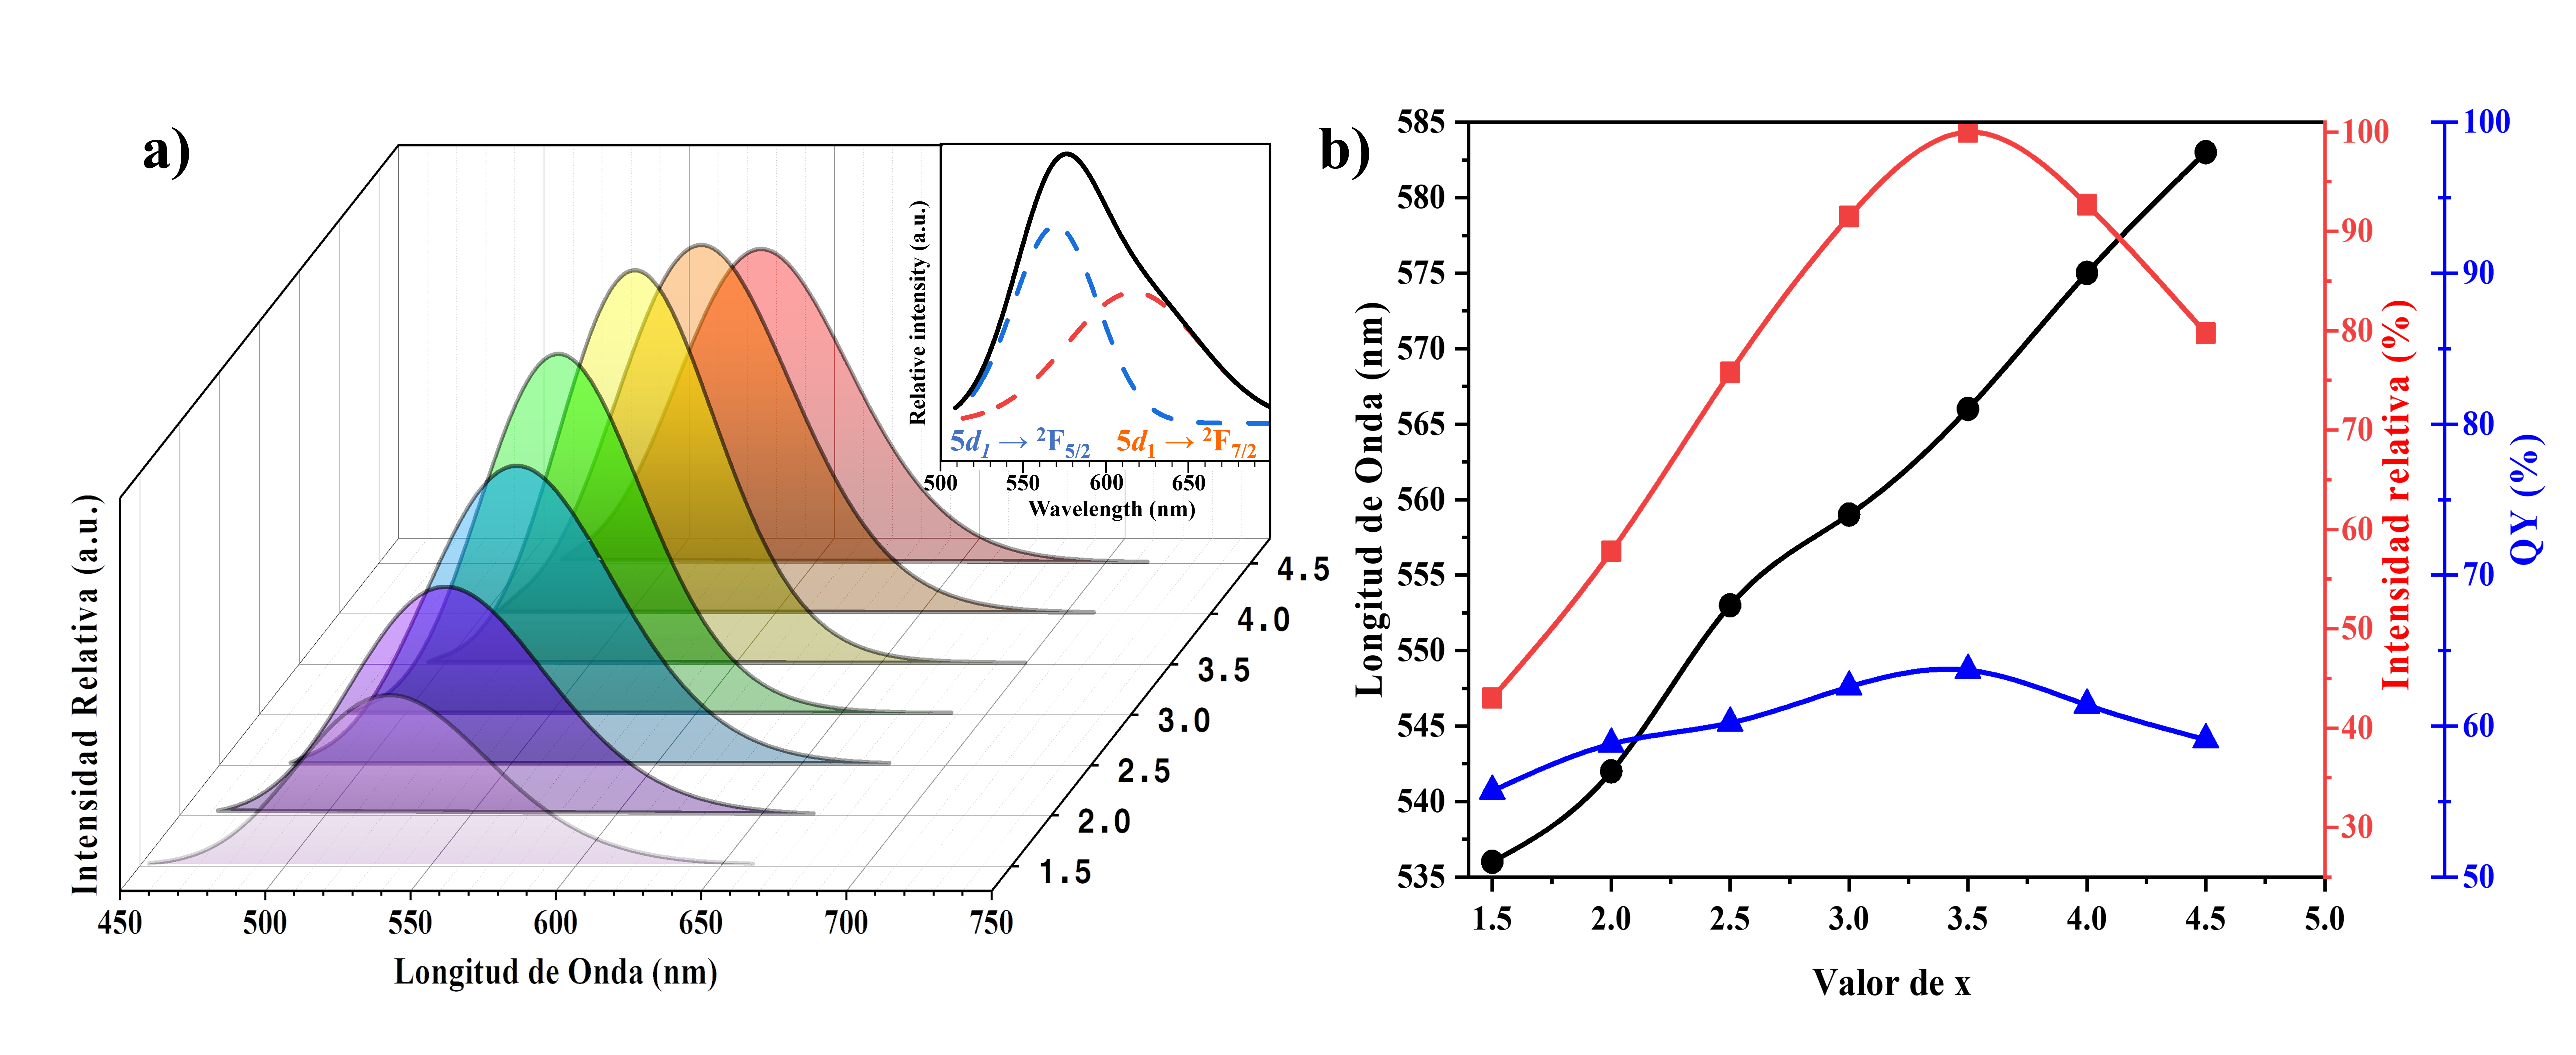
\includegraphics[width=\textwidth]{Kap4/Fotoluminisencia.png}%
    \caption{Espectros de fotoluminiscencia bajo excitación de 436 nm de las
    muestras \ce{Lu3Al_{5-X}Fe_{x}O12}:\ce{Ce^{3+}} con 1.5 $\leq x \leq  $ 4.5
    (a). Longitud de onda, intensidad de emisión y rendimiento cuántico de la
    banda
    de emisión en función del valor x (b). perfiles gaussianos atribuidos a las
    transiciones más bajas de $^2E_g(5d_1)\rightarrow ^2F_{5/2}$ y $^2E_g(5d_1)
        \rightarrow ^2F_{7/2}$ de \ce{Ce^{3+}}}\label{fig:foto}
\end{figure}

Se observó un ligero desplazamiento hacia el rojo al aumentar la concentración
de \ce{Fe^{3+}} (Figura \ref{fig:foto} b), que se atribuye a la energía
$\Delta_{1-2}$
intensificada,
generando una menor separación entre el nivel más bajo de $^2E_g(5d_1)$ y los
estados fundamentales $4f(^2F_{5/2}$ y $^2F_{7/2})$ \cite{Chen2015a,Hu2019}.
Como se
informó
anteriormente, la inserción de \ce{Fe^{3+}} condujo a la expansión de la celda
unidad
y, por lo tanto, se esperarían fenómenos de desplazamiento hacia el azul
\cite{Ueda2019,Dorenbos2013}, y se ajusta a los resultados presentados en
trabajos de
investigación
similares, en los que se insertan cationes más grandes en las estructuras del
granate huésped \cite{Chen2015a,Kamada2011,Hu2015}. Además de la energía
$\Delta_{1-2}$
intensificada, el
desplazamiento al rojo de los espectros de emisión puede atribuirse al aumento
del desplazamiento de Stokes (SS) dentro de los estados fundamentales y el
estado excitado más bajo ($5d_1$). La energía de desplazamiento de Stokes es
proporcional al grado de interacción electrón-fonón \cite{Ueda2019}. Entonces,
la
interacción electrón-fonónica se haría más fuerte al aumentar la concentración
de \ce{Fe^{3+}}, lo que conduciría a un aumento en el desplazamiento de Stokes.
La
banda de emisión de los materiales y los valores del desplazamiento de Stokes
se presentan en la Tabla \ref{tab:emision}.\\

\begin{table}[]
    \caption{Banda de emisión y desplazamiento de Stokes de \ce{Lu3Al_{5-X}Fe_{x}O12}:\ce{Ce^{3+}}}
    \label{tab:emision}
    \resizebox{\textwidth}{!}{%
        \begin{tabular}{cccc}
            \hline
            Valor de x & Banda de Emisión (nm) & Desplazamiento de Stokes (nm)
                       &
            Desplazamiento de Stokes (eV)
            \\ \hline
            
            1.5       & 536 (2.31)         & 88
                       & 0.45
            \\
            2.0       & 542 (2.29)         & 90
                       & 0.46
            \\
            
            2.5       & 553 (2.24)         & 99
                       & 0.49
            \\
            3.0       & 559 (2.22)         & 103
                       & 0.50
            \\
            
            3.5       & 566 (2.19)         & 108
                       & 0.51
            \\
            4.0       & 575 (2.16)         & 115
                       & 0.54
            \\
            
            4.5       & 583 (2.13)         & 120
                       & 0.55
            \\ \hline
        \end{tabular}%
    }
\end{table}

Para aplicaciones de w-LED, el rendimiento cuántico (QY) es un parámetro
importante en la evaluación de fósforos empleados para fabricación de w-LED. El
QY se midió por debajo de 436 nm y se calculó usando la ecuación
\ref{eqn:eq3} \cite{Liu2013}.\\

\begin{equation}
    \eta_{QY} =\frac{\int L_s}{\int E_R-\int E_s}
    \label{eqn:eq3}
\end{equation}

Donde $L_s$ es el espectro de emisión de la muestra, $E_s$ y $E_R$ representan
la luz de excitación con y sin la muestra en la esfera integradora,
respectivamente. El
valor para $\eta_{QY}$ de los materiales aumentó progresivamente, alcanzando un
máximo del 64\% para el material con x = 3.5 (Figura \ref{fig:foto} b). Aunque los valores
de
$\eta_{QY}$ no son tan altos como los del granate comercial
\ce{Y3Al5O12}:\ce{Ce^{3+}},
son más altos que los reportados en otros estudios y podría mejorarse ajustando
las
propiedades estructurales y morfológicas. El aumento de la concentración de
\ce{Fe^{3+}} también generó una mayor intensidad de emisión debido a la
absorción
mejorada a 436 nm (Figura \ref{fig:foto} b), alcanzando un máximo cuando x =
3.5.\\

Los valores máximos de $\eta_{QY}$ y de intensidad de emisión cuando x = 3.5
pueden atribuirse a modos de fonón inaccesibles debido a la inserción de un
sustituyente grande como \ce{Fe^{3+}} en la estructura rígida
\cite{George2013}. (x = 4.0 y
4.5) se deben al hecho de que la inserción de \ce{Fe^{3+}} en la estructura
anfitrión generó la expansión del parámetro de red, aumentando la probabilidad
de transferencia
no radiativa entre cationes \ce{Ce^{3+}} \cite{Chen2015a}. La distancia crítica
($R_c$)
entre cationes \ce{Ce^{3+}} determina cuál mecanismo es responsable de la
extinción, el valor
de ($R_c$) se estimó utilizando la siguiente ecuación \cite{Blasse1968}:\\

\begin{equation}
    R_c \approx 2\left(\frac{3V}{4 \pi X_c N}\right)^{-3}
    \label{eqn:eq4}
\end{equation}

Donde $V$ es el volumen de celda unitaria de la red del anfirión
($V=1797.57$\r{A}$^3$), $N$ es el número de sitios dopantes disponibles en la
celda
unitaria ($N=24$) y $X_c$ es la concentración de cationes \ce{Ce^{3+}}
($X_c=0.045$). El
valor de $R_c$ fue de $14.70$ \r{A} aproximadamente, lo que implica que la
extinción de la
concentración se debe a la interacción eléctrica multipolar
\cite{Li2018,Hua2016}.\\

Las coordenadas de cromaticidad CIE se determinaron a partir de los espectros
de emisión de las muestras y se calculó la pureza del color usando la siguiente
ecuación \cite{KaviRasu2017}:\\

\begin{equation}
    PurezaColor = \sqrt{\frac{(x-x_n)^2+(y-y_n)^2}{(x_i-x_n)^2+(y_i-y_n)^2}}
    \times 100\%
    \label{eqn:eq5}
\end{equation}

Donde ($x$, $y$) son las coordenadas de cromaticidad CIE, ($x_n$, $y_n$) se
refiere a las coordenadas de cromaticidad CIE para el color blanco y ($x_i$,
$y_i$) son las
coordenadas de la longitud de onda dominante.\\

La Tabla \ref{tab:croma} enumera las coordenadas de cromaticidad CIE
y la pureza del color bajo excitación de 436 nm para los materiales
\ce{Lu3Al_{5-X}Fe_{x}O12}:\ce{Ce^{3+}}. Se pudo observar que el dopaje con
\ce{Fe^{3+}} permite aumentar
la pureza del color hasta un 95.2\% (x = 4.5).\\

\begin{table}[]
    \centering
    \caption{Coordenadas cromáticas CIE y pureza color para las muestras \ce{Lu3Al_{5-X}Fe_{x}O12}:\ce{Ce^{3+}} $(1.5\leq x\leq 4.5)$}
    \label{tab:croma}
    \begin{tabular}{llll}
    \hline
         & \multicolumn{2}{l}{Coordenadas CIE} &       \\ \cline{2-3}
    \multirow{-2}{*}{Valor de x} & x & y & \multirow{-2}{*}{Pureza del Color} \\ \hline
    0.15 & 0.3112           & 0.6002           & 77.7\% \\
     
    0.20 & 0.3504           & 0.5917           & 82.3\% \\
    0.25 & 0.3893           & 0.5710           & 88.1\% \\
     
    0.30 & 0.4201           & 0.5508           & 93.1\% \\
    0.35 & 0.4291           & 0.5504           & 93.1\% \\
     
    0.40 & 0.4612           & 0.5321           & 94.8\% \\
    0.45 & 0.4817           & 0.510            & 95.2\% \\ \hline
    \end{tabular}
    \end{table}

Por otro lado, el diagrama de cromaticidad CIE presentado en la Figura
\ref{fig:croma}
muestra que la emisión se ajustó de verde a naranja por el dopaje \ce{Fe^{3+}}
en los
granates.\\

\begin{figure}[t!]
    \centering%

    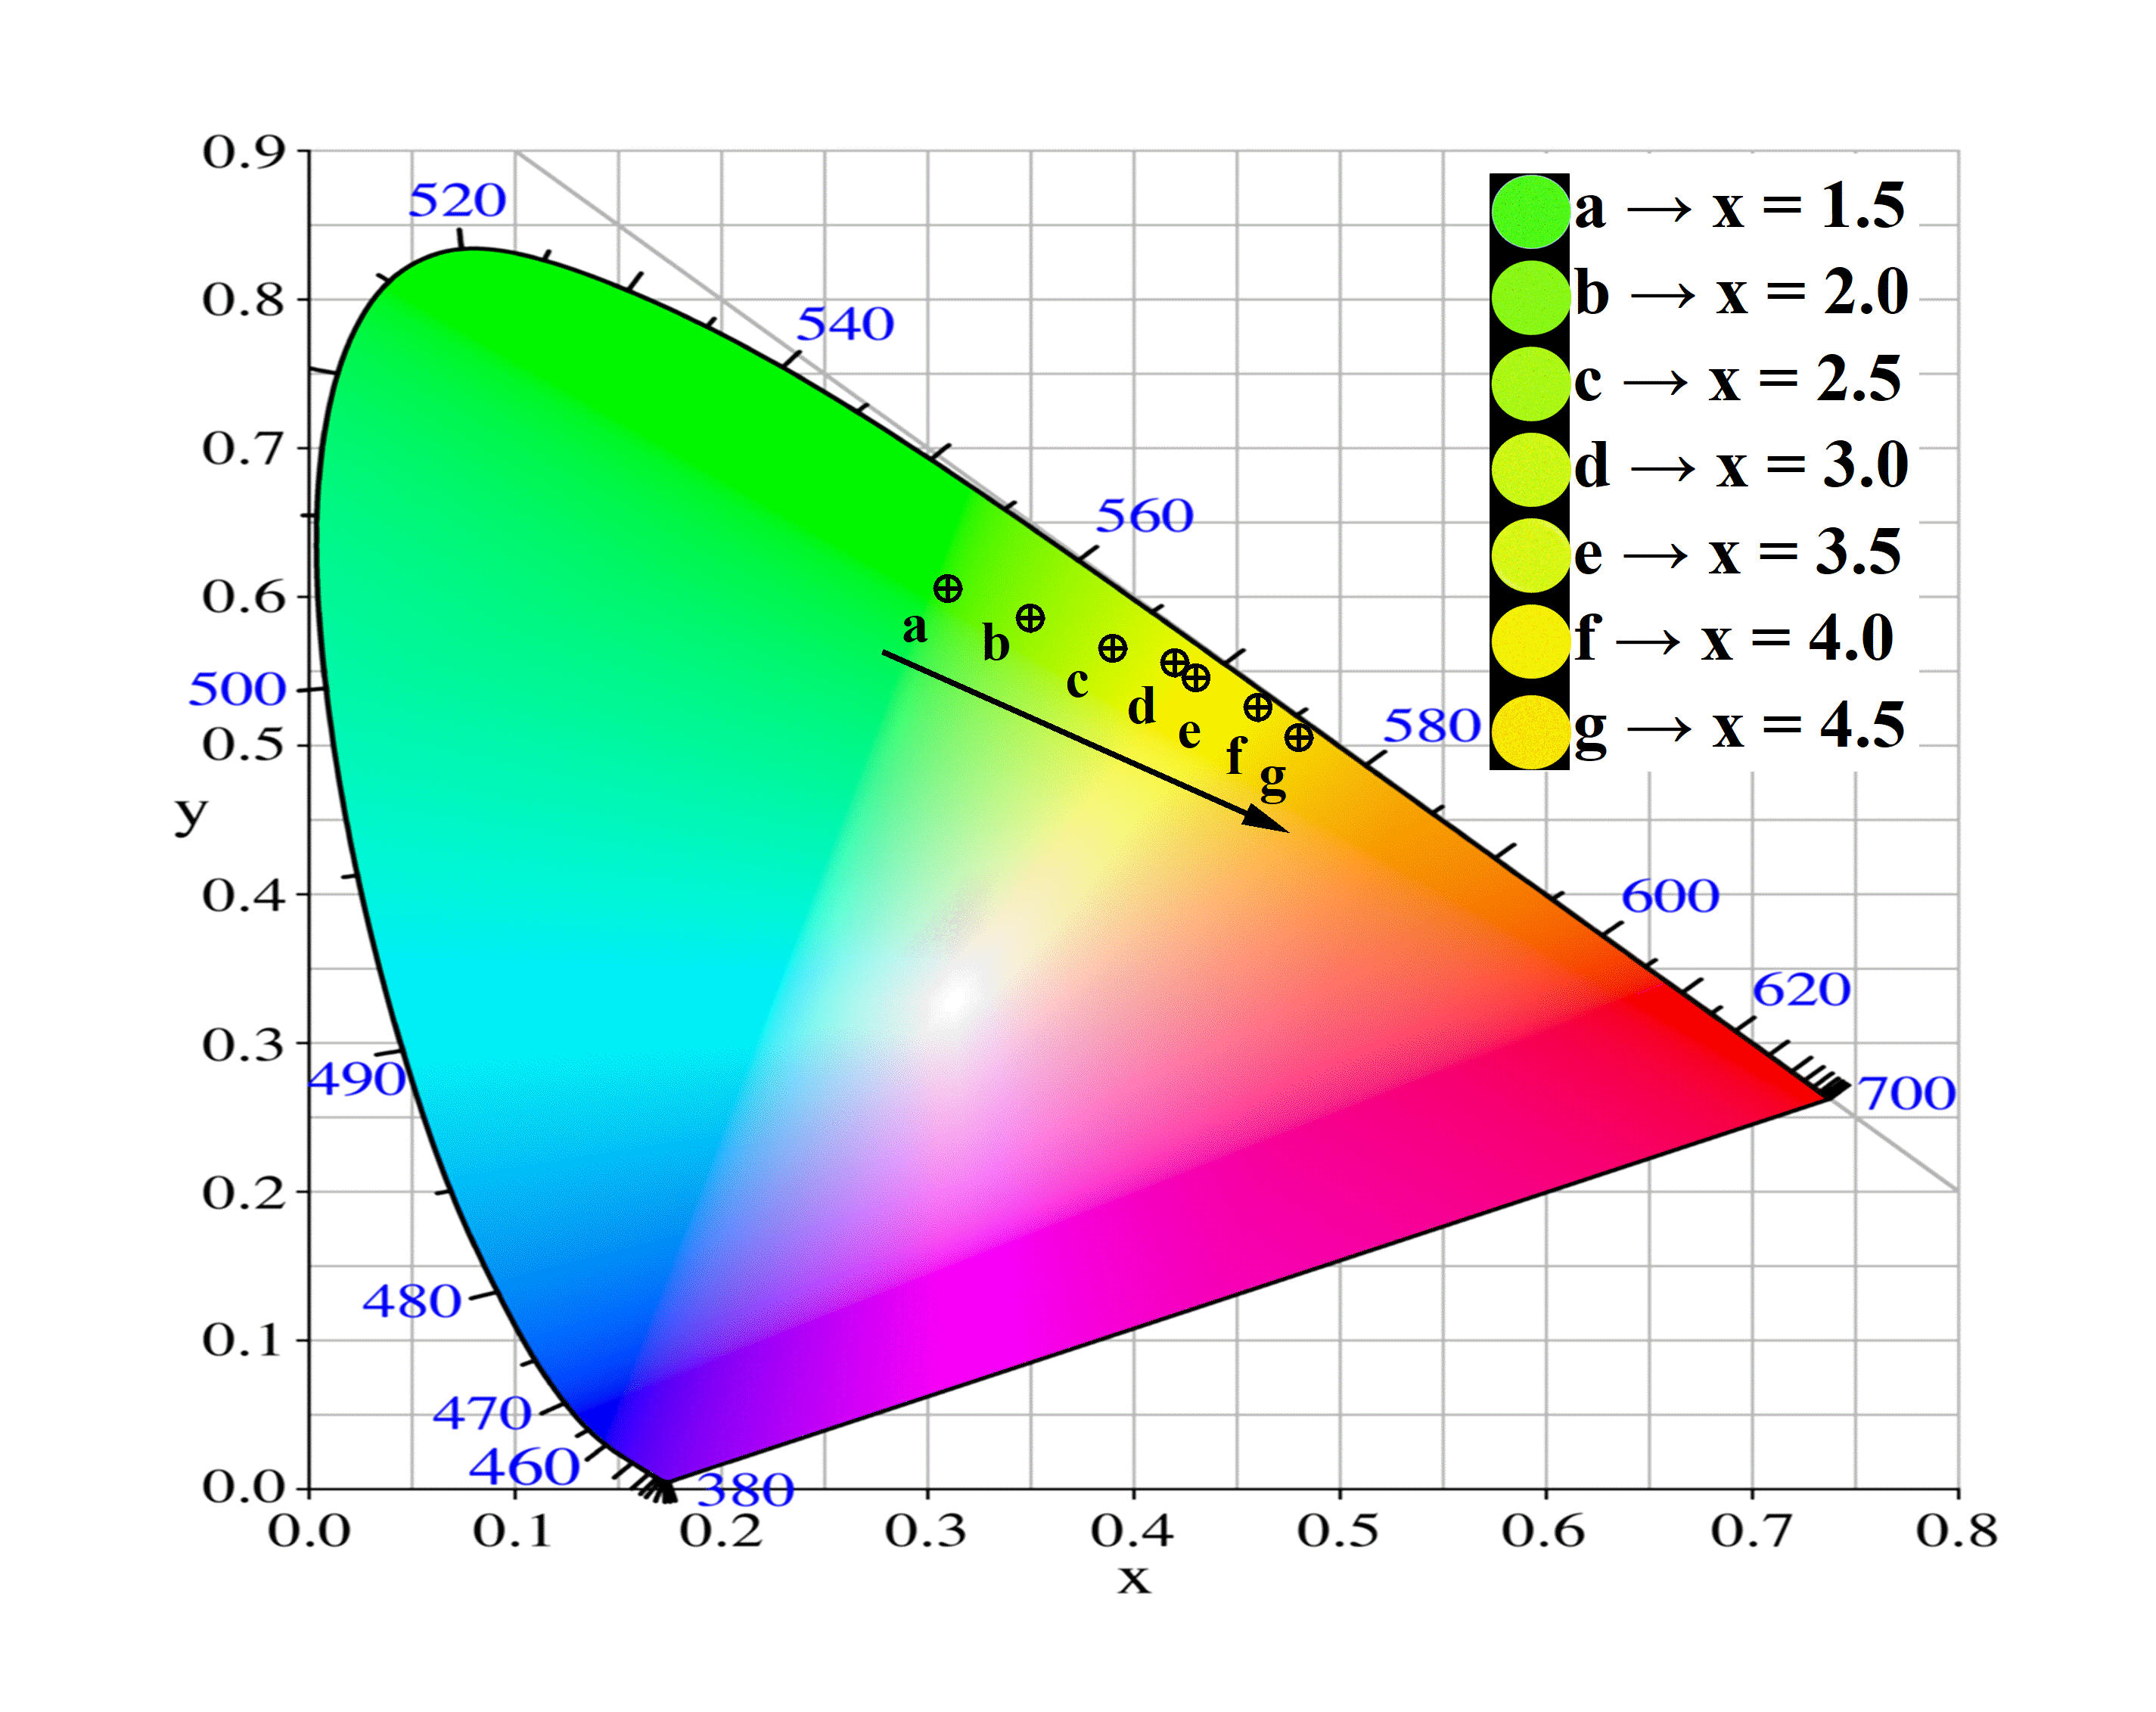
\includegraphics[width=\textwidth]{Kap4/Cromaticidad.png}%
    \caption{Diagrama de cromaticidad CIE para las muestras de
    \ce{Lu3Al_{5-X}Fe_{x}O12}:\ce{Ce^{3+}}	$(1.5\leq x\leq
        4.5)$}\label{fig:croma}
\end{figure}

Los materiales obtenidos exhibieron una gran conversión de color y una alta
pureza de color bajo radiación de luz azul, demostrando sus potenciales
aplicaciones en w-LED. Además, según el análisis óptico, la Figura
\ref{fig:niveles}
muestra
una representación esquemática del efecto
del dopaje con \ce{Fe^{3+}} sobre los niveles de energía de \ce{Ce^{3+}} en los
granates
\ce{Lu3Al_{5-X}Fe_{x}O12}:\ce{Ce^{3+}}.\\

\begin{figure}[h]
    \centering%

    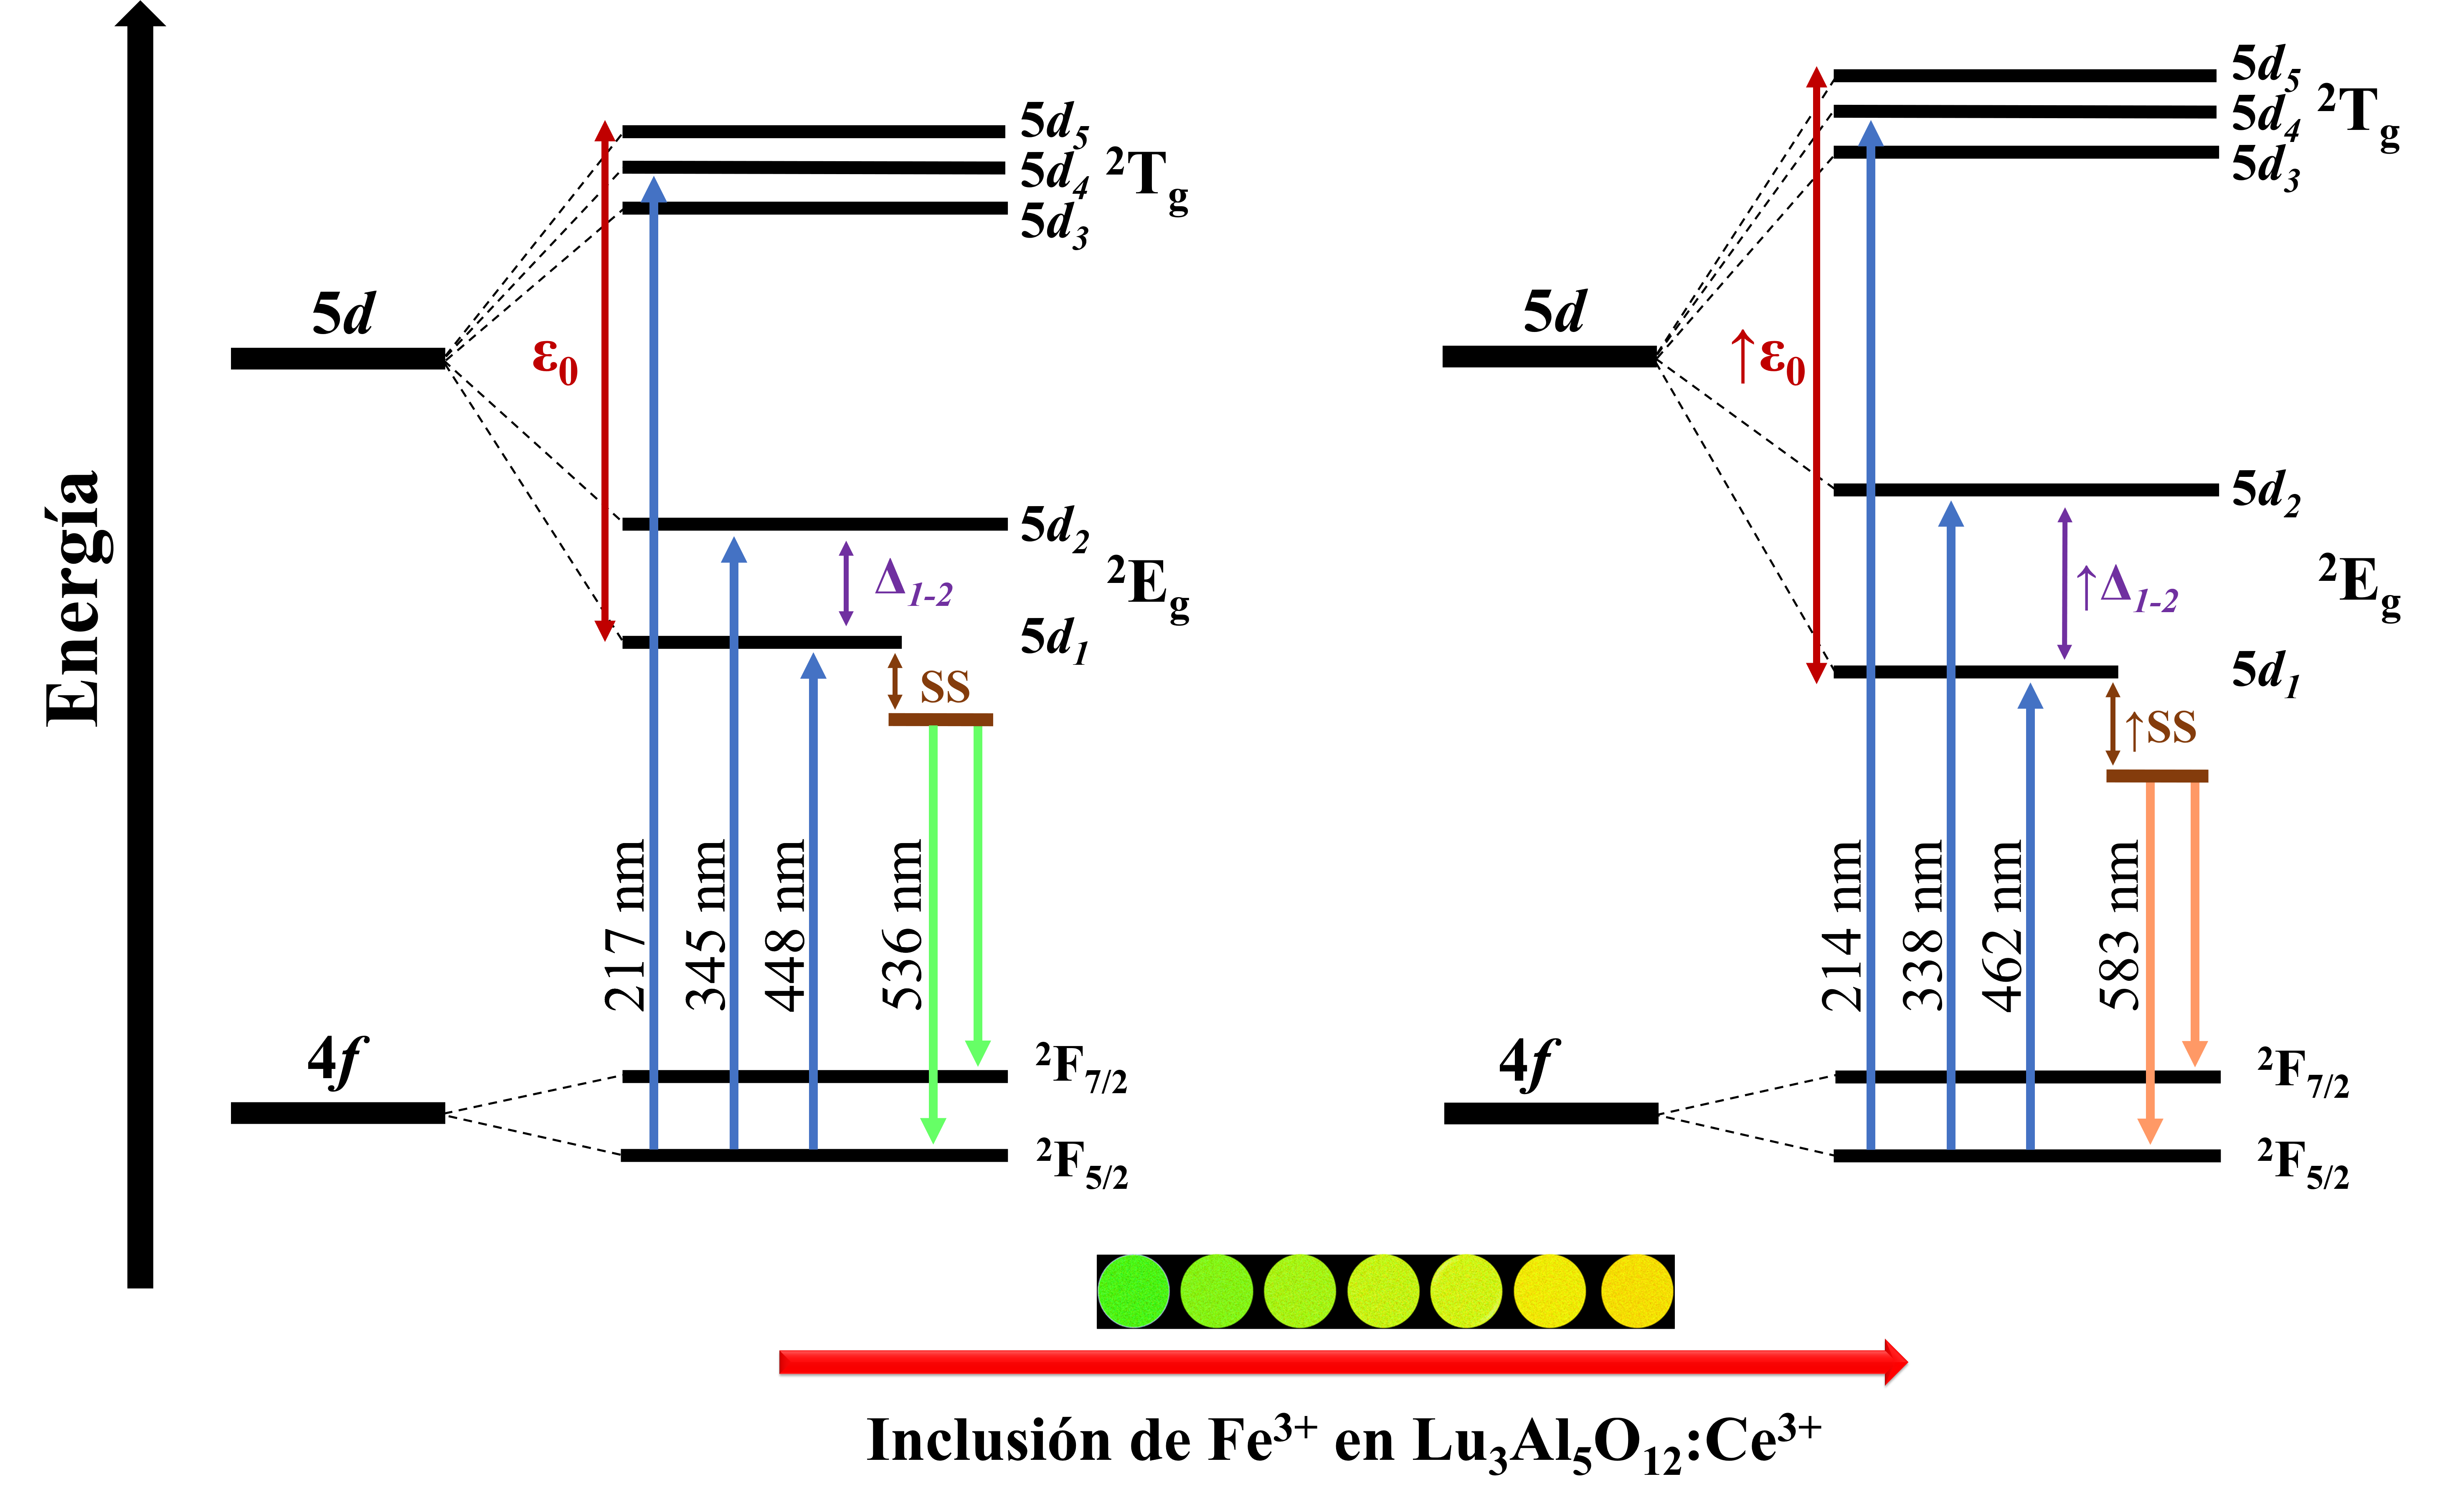
\includegraphics[width=\textwidth]{Kap4/NivelesEnergia.png}%
    \caption{Efecto de la sustitución de \ce{Fe^{3+}} por \ce{Al^{3+}} sobre
    los niveles de energía de \ce{Ce^{3+}} en los granates
    \ce{Lu3Al_{5-X}Fe_{x}O12}:\ce{Ce^{3+}}}\label{fig:niveles}
\end{figure}

Relación entre Temperatura y Fotoluminiscencia: al trabajar con w-LED, la capa
de fósforo puede alcanzar temperaturas de hasta 150$^{\circ}$C. Entonces, la
estabilidad térmica del fósforo es el parámetro más importante para evaluar su
desempeño para aplicaciones w-LED, especialmente aquellos que emplean en su
fabricación chips que emiten luz azul. Los espectros de fotoluminiscencia en
función de la temperatura para el fósforo
\ce{Lu3Al_{5-X}Fe_{x}O12}:\ce{Ce^{3+}} (para x = 3.5)
bajo una excitación de 436 nm se presentan en la Figura \ref{fig:fotoTemp} a)
La intensidad de
emisión disminuyó gradualmente de (25 a 200)$^{\circ}$C debido a los fenómenos de
apagamiento (ver gráfico anexo a Figura \ref{fig:fotoTemp} a). A 150$^{\circ}$C, la
intensidad de
emisión fue del 82.36\% de la intensidad inicial, lo que sugiere un rendimiento
prometedor en el rango de temperatura de funcionamiento de los w-LED. Por otro
lado, la longitud de onda se mantuvo casi sin cambios, lo que demuestra la alta
estabilidad de la emisión de color. El ligero desplazamiento hacia el azul es
atribuible a la excitación asistida por fonones activada térmicamente
\cite{Xia2011}\\

\begin{figure}[h]
    \centering%

    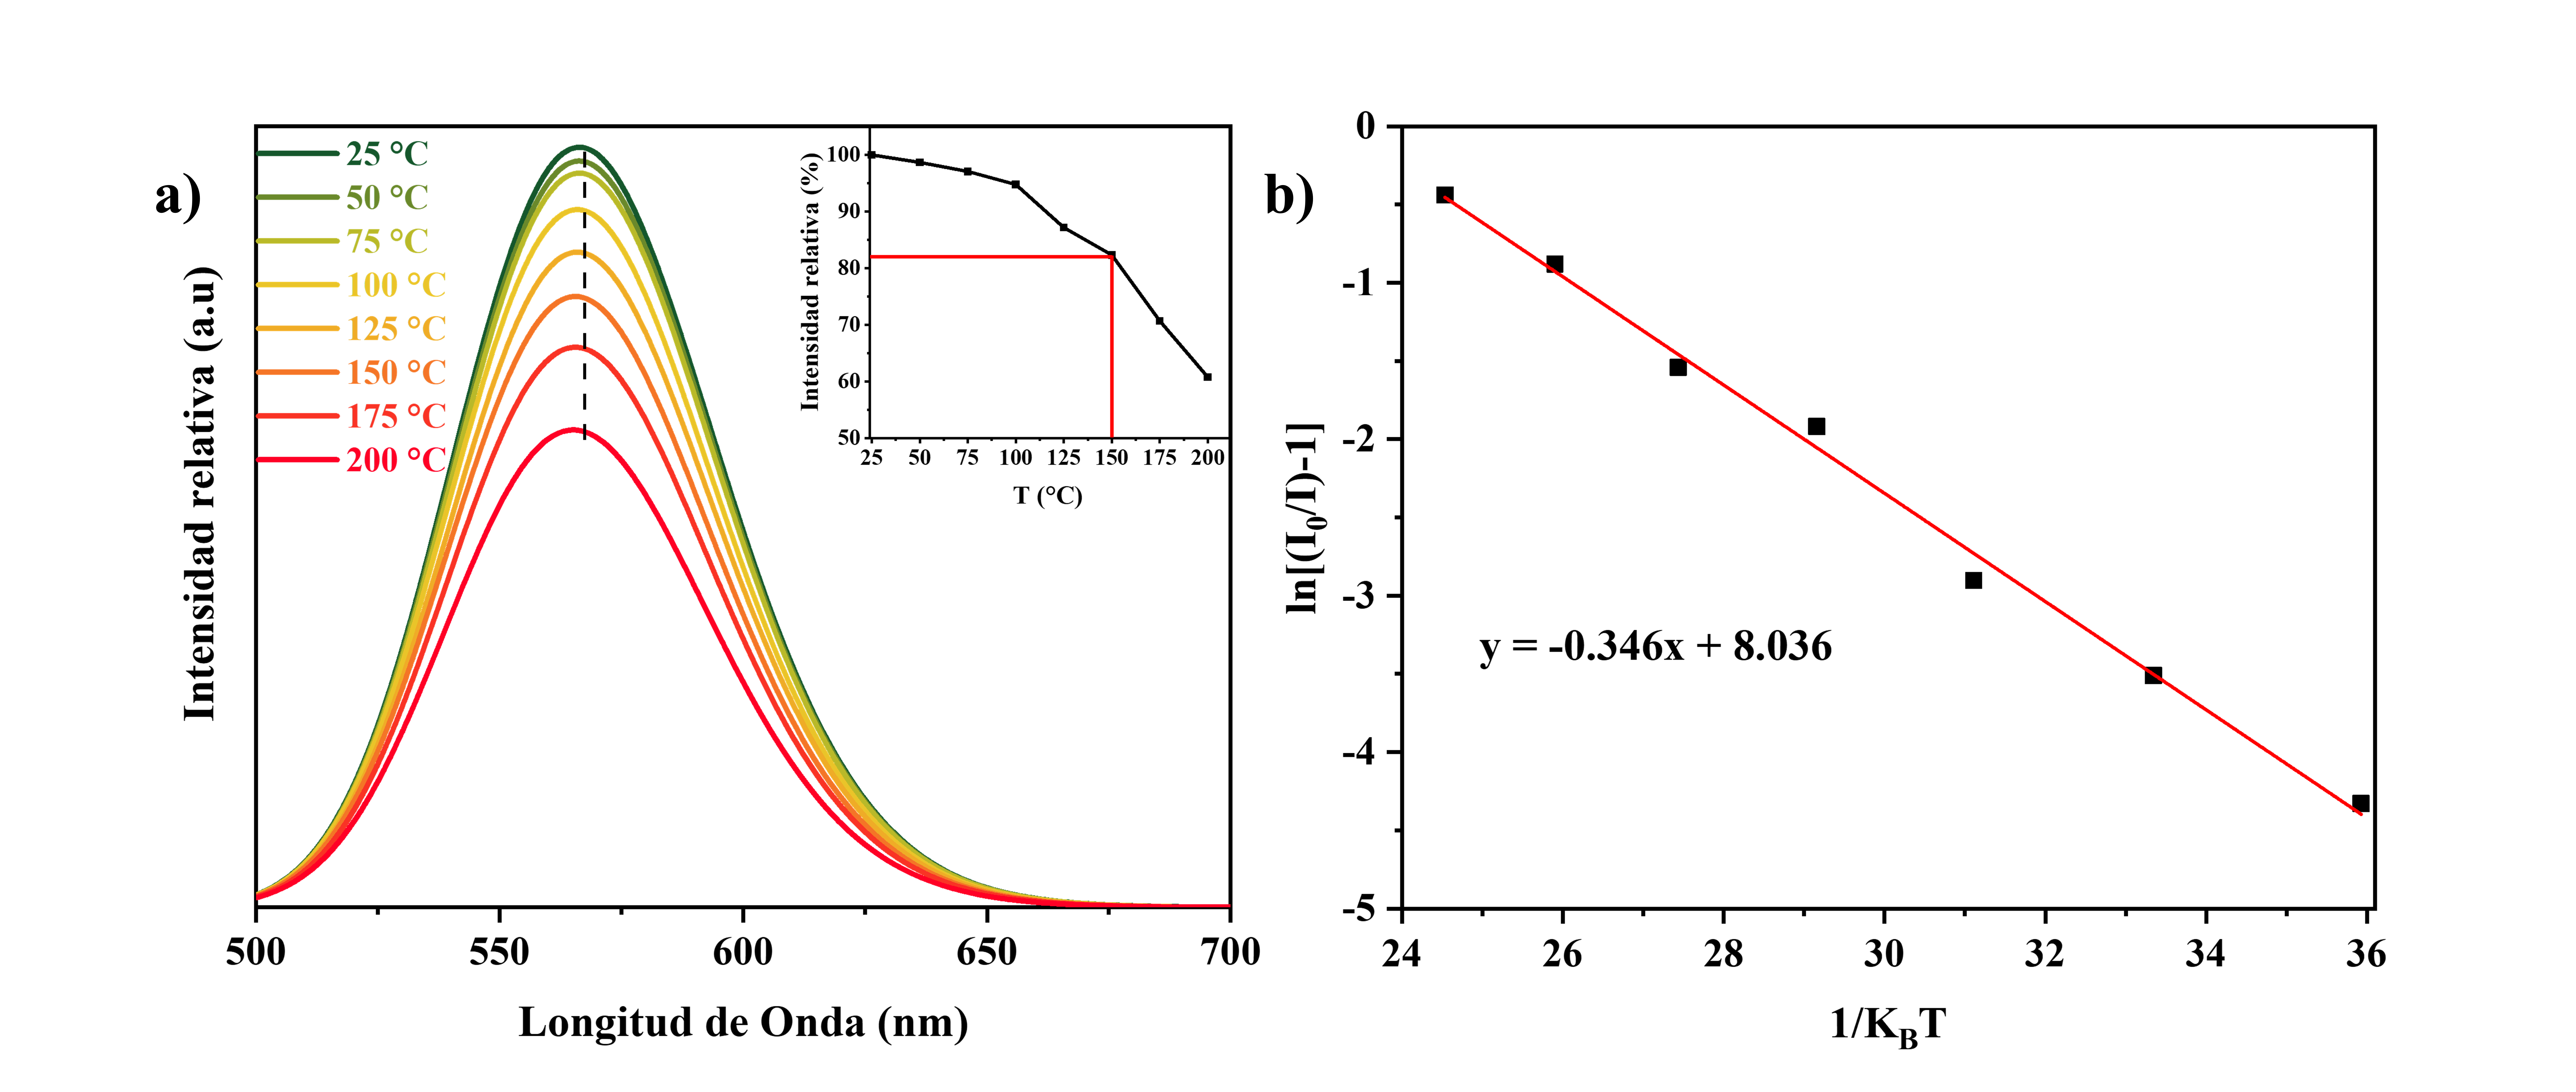
\includegraphics[width=\textwidth]{Kap4/fotoTemperatura.png}%
    \caption{Espectros de fotoluminiscencia en función de la temperatura para
    el fósforo \ce{Lu3Al_{1.5}Fe_{3.5}O12}:\ce{Ce^{3+}} (x = 3.5) bajo
    excitación
    de 436 nm, (a) Intensidad de emisión relativa en función de la temperatura.
    (b)
    Gráfica de $\ln[(I_{0}/I)-1]$ en función de $1/K_BT$}\label{fig:fotoTemp}
\end{figure}

La energía de activación ($\Delta E$) se calculó mediante la ecuación Arrhenius
(\ref{eqn:eq6}) \cite{Chen2015}.\\

\begin{equation}
    I=\frac{I_0}{1+A e^{-\Delta E/K_BT}}
    \label{eqn:eq6}
\end{equation}

Donde $I$ e $I_0$ indican la intensidad de emisión a la temperatura T y la
temperatura inicial (en escala absoluta), respectivamente. $A$ es una constante
y
$K_B$ es la constante de Boltzmann ($8.629×10^{-5} eV^{-1}$). $\Delta E$ se
determina mediante el
valor absoluto de la pendiente para la gráfica de $\ln [(I_0/I)-1] $ en función
a $1/K_{B}T$ (Figura \ref{fig:fotoTemp} b). El valor obtenido de $\Delta E$ fue
de $0.346 eV$, que es relativamente
alto y
muestra propiedades térmicas sobresalientes.\\
\chapter{Caracterización Morfológica y Composicional}
\label{MEB}
Se eligieron las muestras con x=0.0, 0.5, 2.5 y 4.5 para realizar la
caracterización morfológica y composicional con aumento desde los 2k a los 90k,
con el fin de ver la variación en la microestructura a medida que se aumentaba
la inclusión de \ce{Fe^{3+}}, además se obtuvieron micrografías con EDX para
determinar las características superficiales de los materiales.\\

\begin{figure}[h]
    \centering%

    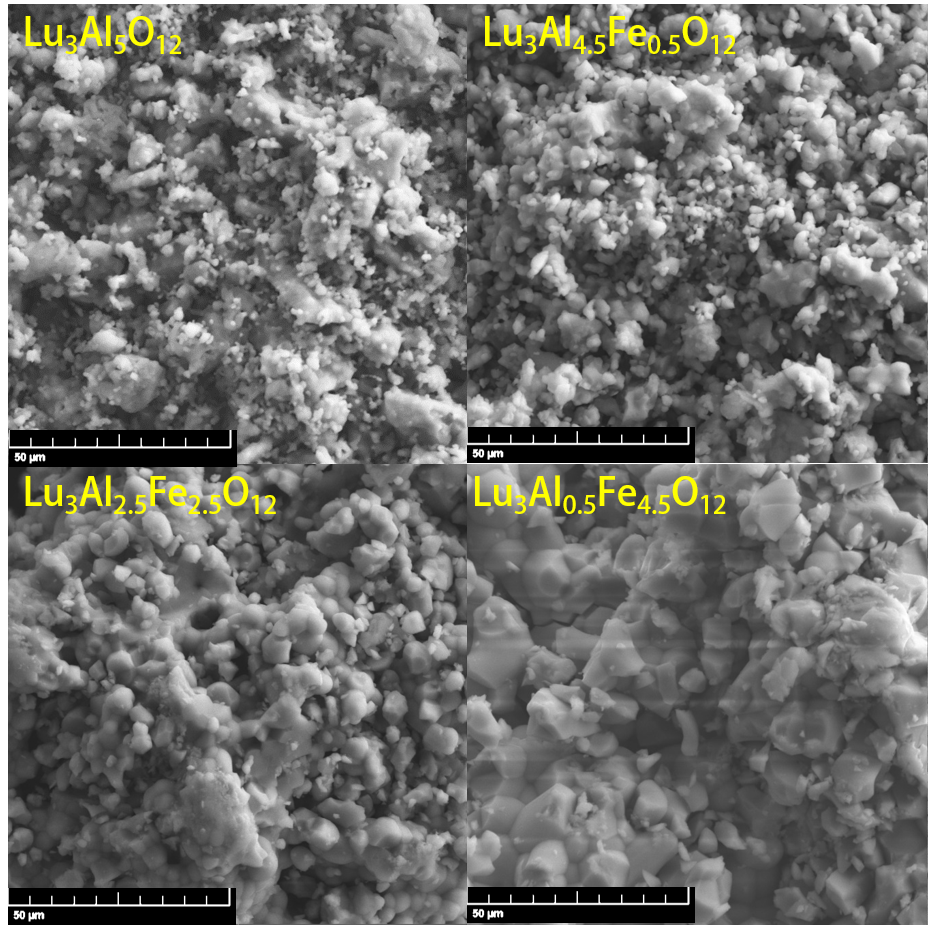
\includegraphics[width=12cm]{Kap5/sec20k.png}%
    \caption{Micrografías con electrones secundarios a 20.000 aumentos para los
    materiales \ce{Lu3Al_{5-X}Fe_{x}O12}:\ce{Ce^{3+}} con x=0.0, 0.5, 2.5
    }\label{fig:sec20}
\end{figure}

En la Figura \ref{fig:sec20} se presentan las micrografías obtenidas con
electrones
secundarios que proporcionan información topográfica de cada
muestra, en donde, se observó la formación de agregados con formas irregulares
y bordes bien definidos.\\

\begin{figure}[h]
    \centering%

    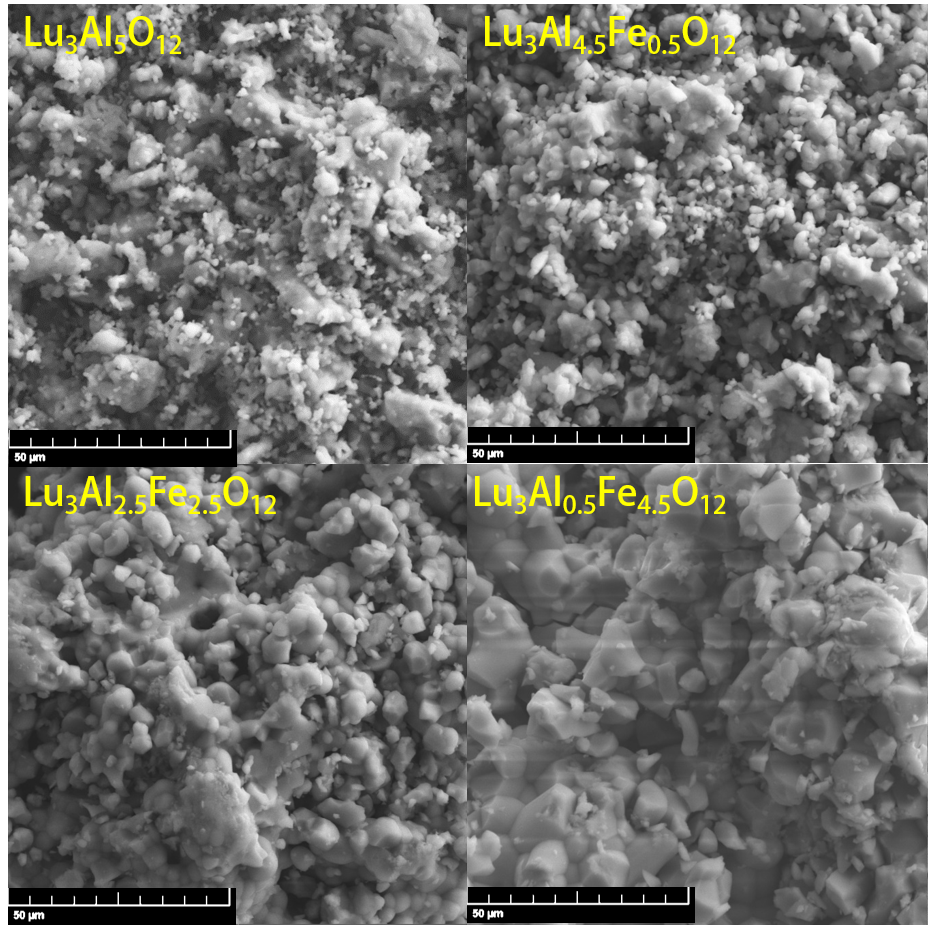
\includegraphics[width=12cm]{Kap5/sec20k.png}%
    \caption{Micrografías con electrones secundarios a 90.000 aumentos para los
    materiales \ce{Lu3Al_{5-X}Fe_{x}O12}:\ce{Ce^{3+}} con x=0.0, 0.5, 2.5
    }\label{fig:sec90}
\end{figure}

En la Figura \ref{fig:sec90} se muestran las micrografías a 90.000 aumentos, en donde, se
observa poco espacio entre partículas, lo que permite confirmar que el proceso
de prensado para obtener las pastillas de cada muestra favoreció la cinética de
densificación. Sin embargo, no se obtuvo la misma densificación para todas las
muestras debido a variación en la composición química y el tamaño de partícula
de los precursores \cite{MoralesRivera2019}. El proceso de prensado ayudó en la difusión y reacción
entre los precursores permitiendo la formación de la fase cristalina deseada y
llevo a una reducción en la temperatura y tiempo de sinterización \cite{Kang2005}.\\

Por medio del software ImageJ se determinó el tamaño promedio aproximado de
partícula de las muestras del sistema \ce{Lu3Al_{5-X}Fe_{x}O12}:\ce{Ce^{3+}} con x = 0.0, 0.5, 2.5 y
4.5 obtenidos por el método cerámico utilizando las imágenes tomadas a 20.000
aumentos. En el Anexo \ref{AnexoD} se muestran las distribuciones aproximadas de tamaño de
partícula obtenidos para cada uno de los materiales del sistema. En donde, se
observó un aumento del tamaño de las partículas a medida que se aumentó el
dopaje con \ce{Fe^{3+}} (ver Figura \ref{fig:sec90}). Por lo tanto se puedo determinar que el tamaño de partícula
aumentó cuando el \ce{Fe^{3+}} se incorporo dentro de la estructura cristalina del 
granate LUAG, por lo tanto, se evidencia una relación entre el tamaño de grano con los radios iónicos. 
Se sabe que el radio iónico del \ce{Fe^{3+}} es mayor que el del \ce{Al^{3+}}. También se identifica que el
tamaño de partícula presenta un comportamiento similar al tamaño de cristalito
calculado mediante el refinamiento Rietveld de los patrones obtenidos por DRX \cite{Akhtar2017a}.
\\

\begin{figure}[h]
    \centering%

    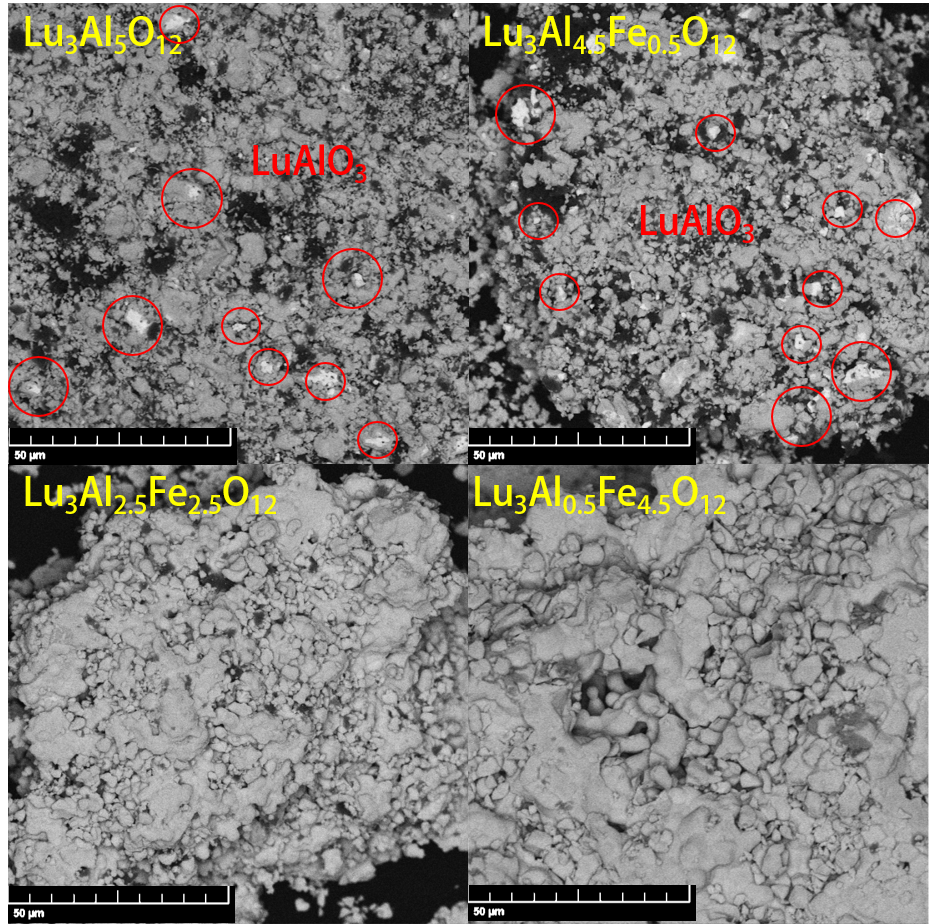
\includegraphics[width=12cm]{Kap5/ret10k.png}%
    \caption{Micrografías con electrones retrodispersados a 10k aumentos. 
    En círculos rojos se señala la presencia de la fase secundaria (\ce{LuAlO2}) }
    \label{fig:ret10}
\end{figure}

En la Figura \ref{fig:ret10} se presentan las micrografías con electrones retro dispersados,
en donde, se puede apreciar que para los materiales \ce{Lu3Al5O12} y
\ce{Lu3Al_{4.5}Fe_{0.5}O12} se observan partículas con una tonalidad más clara que se
asocia con la presencia de la fase secundaria \ce{LuAlO3} que se identificó mediante
la difracción de rayos X y el refinamiento Rietveld, igualmente se confirma la
pureza para $x\leq 2.5$, mediante las micrografías de los materiales
\ce{Lu3Al_{2.5}Fe_{2.5}O12} y \ce{Lu3Al_{0.5}Fe_{4.5}O12}, donde, se tiene uniformidad en la
composición de todas las partículas.\\


\begin{figure}[t]
    \centering%

    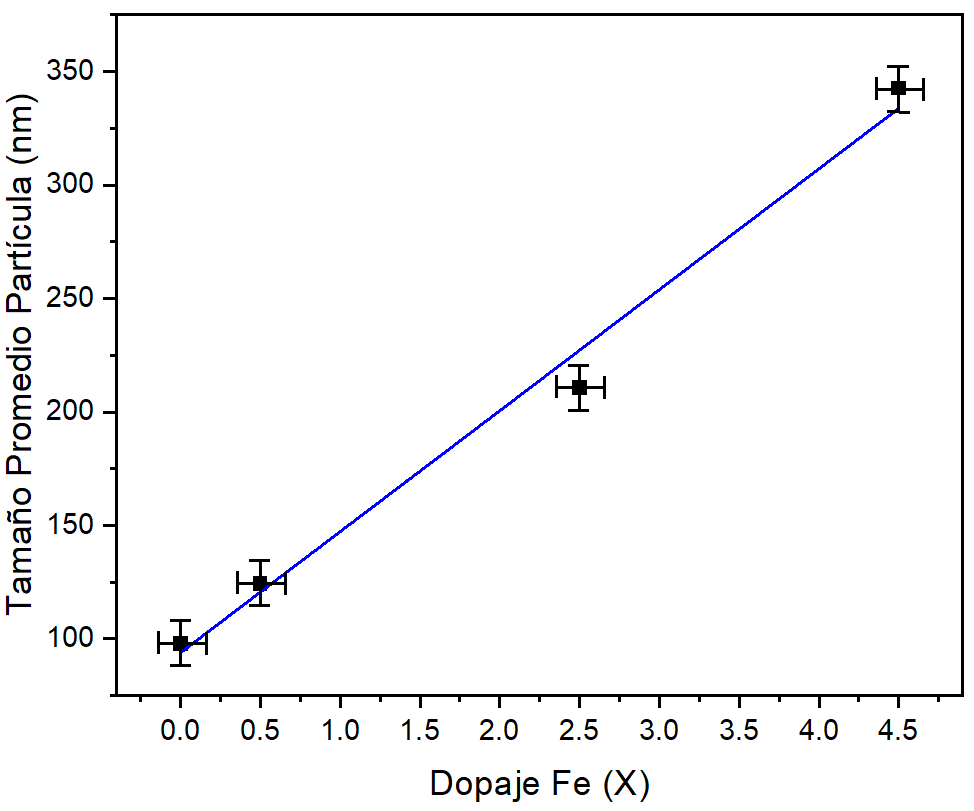
\includegraphics[width=12cm]{Kap5/TamPar.png}%
    \caption{Tamaño de partícula en función del dopaje con \ce{Fe^{3+}}
    }\label{fig:tamfe}
\end{figure}

\begin{table}[h]
    \caption{Porcentaje atómico teórico y experimental obtenido de los resultados de EDX}
    \label{tab:porce}
    %\resizebox{\textwidth}{!}{%
    \begin{tabular}{cccccc}
    \hline
    \multirow{2}{*}{Valor   de x} & \multirow{2}{*}{Formula} & \multicolumn{4}{c}{\% Atomico Teorico   (Experimental)} \\ \cline{3-6} 
        &                             & Lu        & Al          & Fe         & O         \\ \hline
    0.0 & \ce{Lu3Al5O12}              & 15(23.63) & 25.0(26.79) & -          & 60(49.58) \\
    0.5 & \ce{Lu3Al_{4.5}Fe_{0.5}O12}  & 15(16.47) & 22.5(20.16) & 2.5(2.4)   & 60(60.97) \\
    2.5 & \ce{Lu3Al_{2.5}Fe_{2.5}O12} & 15(22.40) & 12.5(10.43) & 12.5(13.2) & 60(53.96) \\
    4.5 & \ce{Lu3Al_{4.5}Fe_{0.5}O12} & 15(20.81) & 2.5(2.63)   & 22.5(27.1) & 60(49.44) \\ \hline
    \end{tabular}%
    %}
\end{table}

Mediante los resultados del análisis semicuantitativo de EDX (ver Anexo \ref{edx}) para las muestras con x=0.0, 0.5, 2.5 y 4.5
se construyó la Tabla \ref{tab:porce} donde se presentan los porcentajes atómicos comparados
con los porcentajes teóricos según la fórmula química. En la Tabla \ref{tab:proporcion} se lista 
la relación lutecio-hierro con el fin de observar mejor la diferencia, de ahí
se puede inferir que el proceso de sinterización fue adecuado, ya que permitió
obtener materiales con una relación aproximada a lo esperado.\\

\begin{table}[h]
    \caption{Proporción Fe/Lu teórica y experimental mediante los resultados de EDX}
    \label{tab:proporcion}
    %\resizebox{\textwidth}{!}{%
    \begin{tabular}{ccccc}
    \hline
    \multirow{2}{*}{Valor de x} & \multirow{2}{*}{Formula} & \multicolumn{2}{c}{Proporción Fe/Al} & \multirow{2}{*}{Diferencia} \\ \cline{3-4}
        &                             & Teórica & Experimental &      \\ \hline
    0.0 & \ce{Lu3Al5O12}              & 0.00    & 0.00         & 0.00 \\
    0.5 & \ce{Lu3Al_{4.5}Fe_{0.5}O12}  & 0.11    & 0.12         & 0.01 \\
    2.5 & \ce{Lu3Al_{2.5}Fe_{2.5}O12} & 1.00    & 1.27         & 0.27 \\
    4.5 & \ce{Lu3Al_{4.5}Fe_{0.5}O12} & 9.00    & 10.31        & 1.31 \\ \hline
    \end{tabular}%
    %}
\end{table}



\include{Kap6/Kap6}
\chapter{Conclusiones y recomendaciones}
\section{Conclusiones}

Se produjeron nuevos granates basados en el sistema
\ce{Lu3Al_{5-X}Fe_{x}O12}:\ce{Ce^{3+}} mediante el método de reacción en estado
sólido a 1200 °C durante 20 h. El dopaje \ce{Fe^{3+}} mejoró la pureza de los
materiales, obteniendo fase pura para valores de $x \geq  2.5$. Se observó una
expansión de la celda unidad y modificaciones en la energía de las absorciones
vibracionales al aumentar la concentración de \ce{Fe^{3+}}, lo que confirma la
adecuada
inserción del \ce{Fe^{3+}} en la estructura del huésped. El análisis óptico
indicó que
el dopaje con \ce{Fe^{3+}} condujo a una fuerte reducción de la banda prohibida
y la
intensificación de la energía del campo cristalino, que eran atribuibles a la
presencia de orbitales moleculares. Además, la fotoluminiscencia de emisión se
ajustó de verde a naranja debido a las modificaciones en los niveles de energía
de \ce{Ce^{3+}}. Los materiales obtenidos exhibieron propiedades ópticas, como
alta
conversión de color, estabilidad térmica, rendimiento cuántico y pureza de
color, que permiten sus posibles aplicaciones en la producción de w-LED.\\

Los resultados de caracterización morfológica realizados por medio de
microscopia electrónica de barrido MEB y el software ImageJ, mostraron que el
tamaño de partículas con forma irregular aumenta de manera proporcional a la
inclusión del \ce{Fe^{3+}} dentro de la estructura del granate, que se
relaciona
directamente con el aumento del tamaño del cristalito identificado mediante
el refinamiento Rietveld, obteniendo materiales con tamaños entre 100 y 350
nm.\\

La inclusión de \ce{Fe} dentro de la estructura del granate LuAG:Ce ajusto la
respuesta
magnética de los materiales, pasando por paramagnética, ferromagnética blanda y
ferromagnética.
Se observó que a mayor tamaño de partícula se tiene un mayor valor de
magnetización de saturación,
logrando 10 emu/g a un campo de 1500 Oe. Para los materiales con respuesta
ferrimagnética
($x \geq 3.5$) se evidencia una disminución de los valores de Mr y Hc a medida
que
aumenta la temperatura. Se observa un aumento significativo de Hc a medida que
la
temperatura disminuye, lo que indica que el material se vuelve magnéticamente
más
duro a menor temperatura.

%\section{Recomendaciones}
%Se presentan como una serie de aspectos que se podr\'{\i}an realizar en un
%futuro para emprender investigaciones similares o fortalecer la
%investigaci\'{o}n realizada. Deben contemplar las perspectivas de la
%investigaci\'{o}n, las cuales son sugerencias, proyecciones o alternativas que
%se presentan para modificar, cambiar o incidir sobre una situaci\'{o}n
%espec\'{\i}fica o una problem\'{a}tica encontrada. Pueden presentarse como un
%texto con caracter\'{\i}sticas argumentativas, resultado de una reflexi\'{o}n
%acerca de la tesis o trabajo de investigaci\'{o}n.\\
\begin{appendix}
	\chapter{Análisis de DRX mediante X'Pert HighScore}\label{AnexoA}

	\begin{figure}[h]
		\centering%
		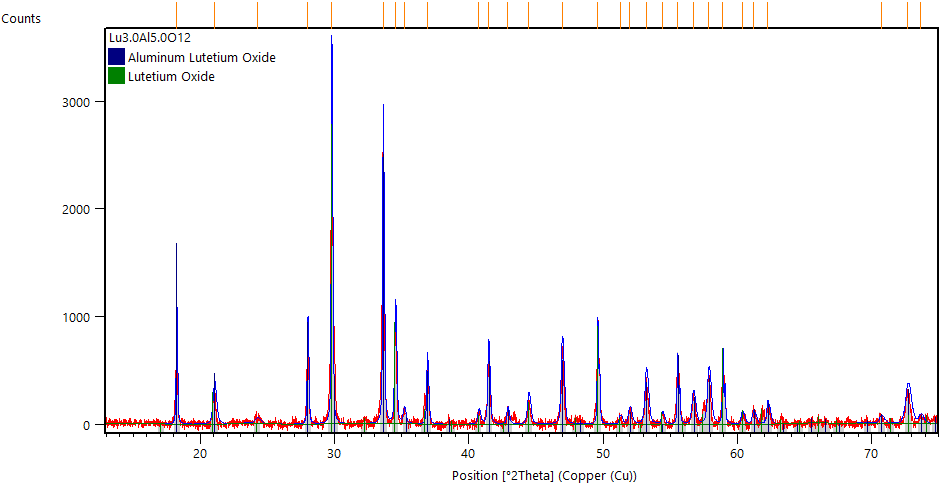
\includegraphics[width=\textwidth]{Anexos/x=0.png}%
		\caption{Análisis del patrón de difracción de rayos X de la muestra
		\ce{Lu_{3.0}Al_{5.0}O12}} \label{fig:XpertX0}
	\end{figure}

	\begin{figure}[h]
		\centering%
		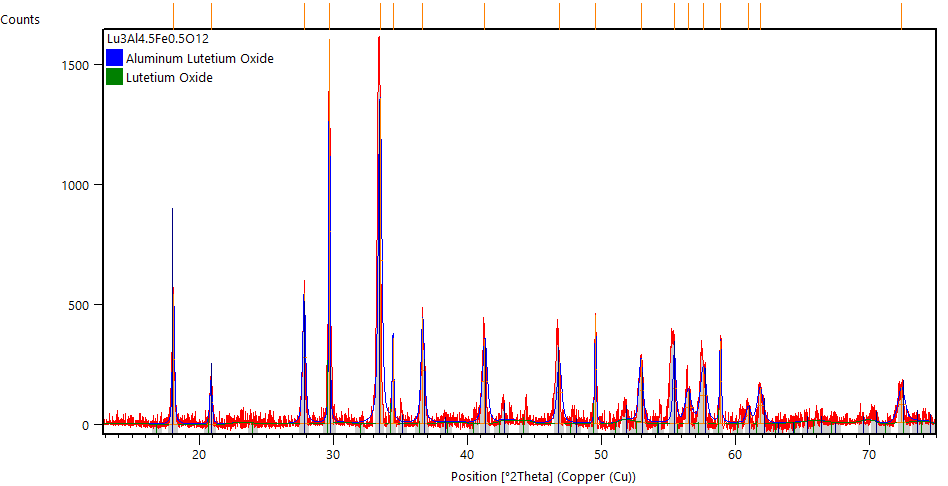
\includegraphics[width=\textwidth]{Anexos/x=05.png}%
		\caption{Análisis del patrón de difracción de rayos X de la muestra
		\ce{Lu_{3.0}Al_{4.5}Fe_{0.5}O12}} \label{fig:XpertX05}
	\end{figure}

	\begin{figure}[h]
		\centering%
		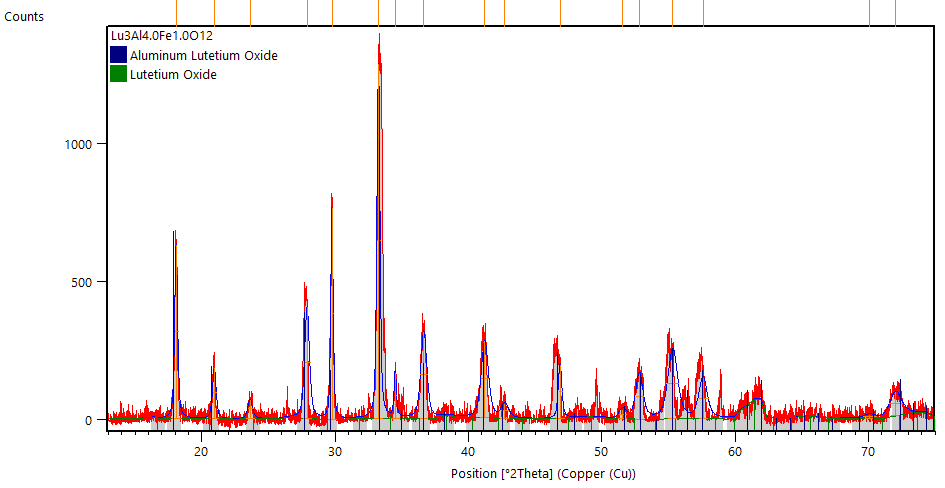
\includegraphics[width=\textwidth]{Anexos/x=10.png}%
		\caption{Análisis del patrón de difracción de rayos X de la muestra
		\ce{Lu_{3.0}Al_{4.0}Fe_{1.0}O12}}
		\label{fig:XpertX10}
	\end{figure}

	\begin{figure}[h]
		\centering%
		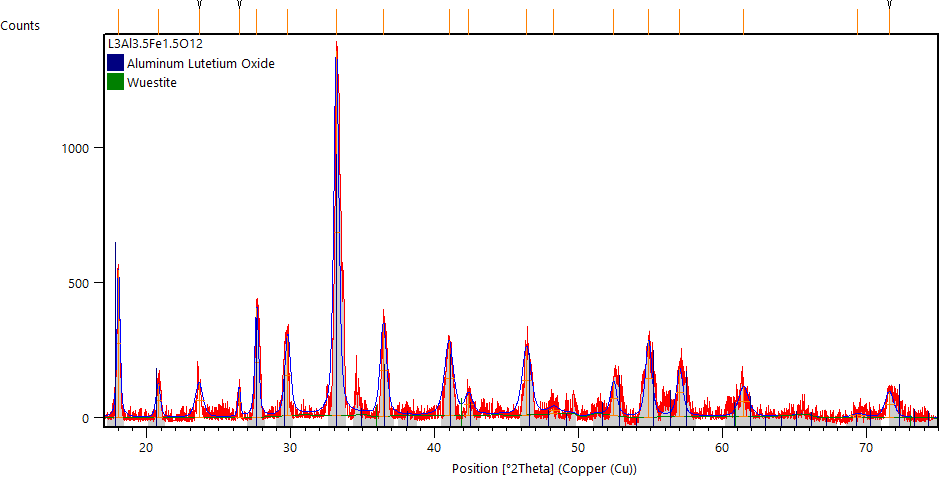
\includegraphics[width=\textwidth]{Anexos/x=15.png}%
		\caption{Análisis del patrón de difracción de rayos X de la muestra
		\ce{Lu_{3.0}Al_{3.5}Fe_{1.5}O12}} \label{fig:XpertX15}
	\end{figure}

	\begin{figure}[h]
		\centering%
		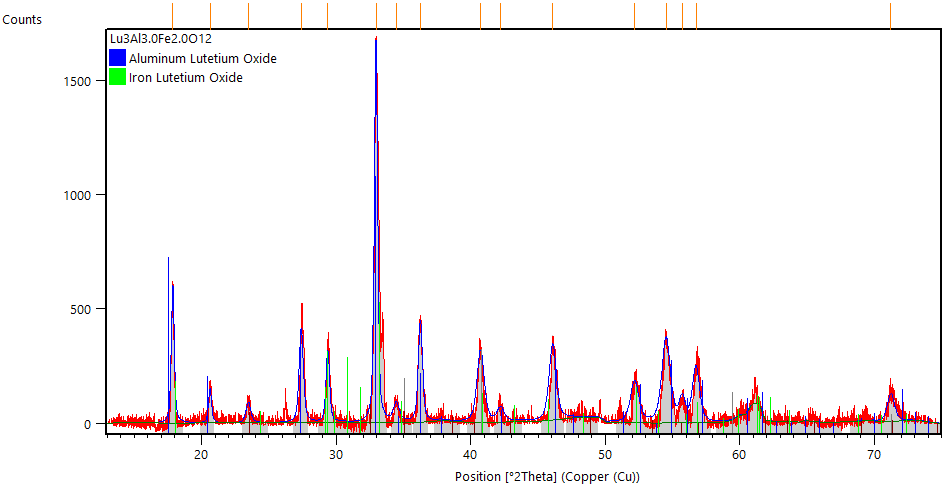
\includegraphics[width=\textwidth]{Anexos/x=20.png}%
		\caption{Análisis del patrón de difracción de rayos X de la muestra
		\ce{Lu_{3.0}Al_{3.0}Fe_{2.0}O12}} \label{fig:XpertX20}
	\end{figure}

	\begin{figure}[h]
		\centering%
		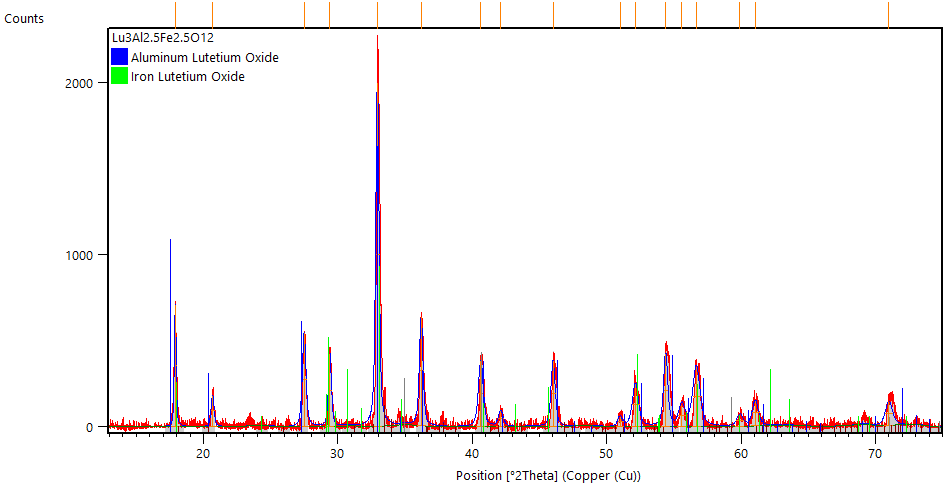
\includegraphics[width=\textwidth]{Anexos/x=25.png}%
		\caption{Análisis del patrón de difracción de rayos X de la muestra
		\ce{Lu_{3.0}Al_{2.5}Fe_{2.5}O12}}  \label{fig:XpertX25}
	\end{figure}

	\begin{figure}[h]
		\centering%
		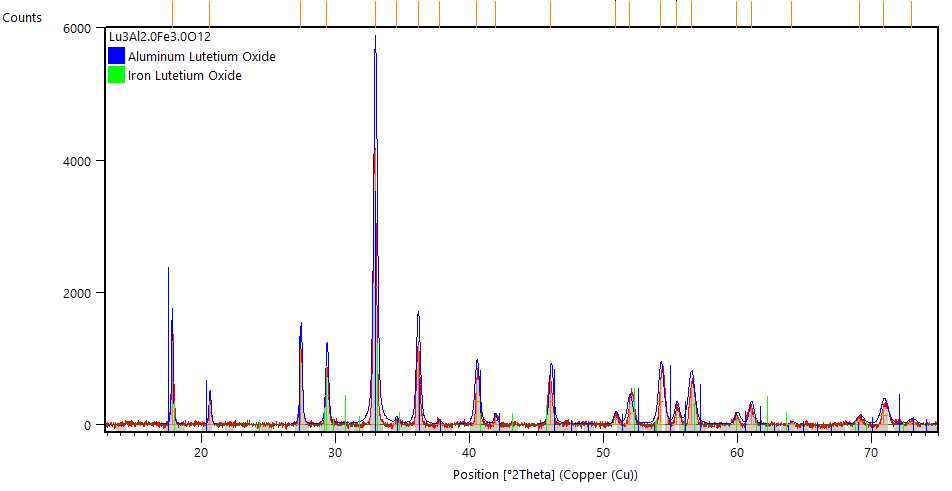
\includegraphics[width=\textwidth]{Anexos/x=30.png}%
		\caption{Análisis del patrón de difracción de rayos X de la muestra
		\ce{Lu_{3.0}Al_{2.0}Fe_{3.0}O12}} \label{fig:XpertX30}
	\end{figure}

	\begin{figure}[h]
		\centering%
		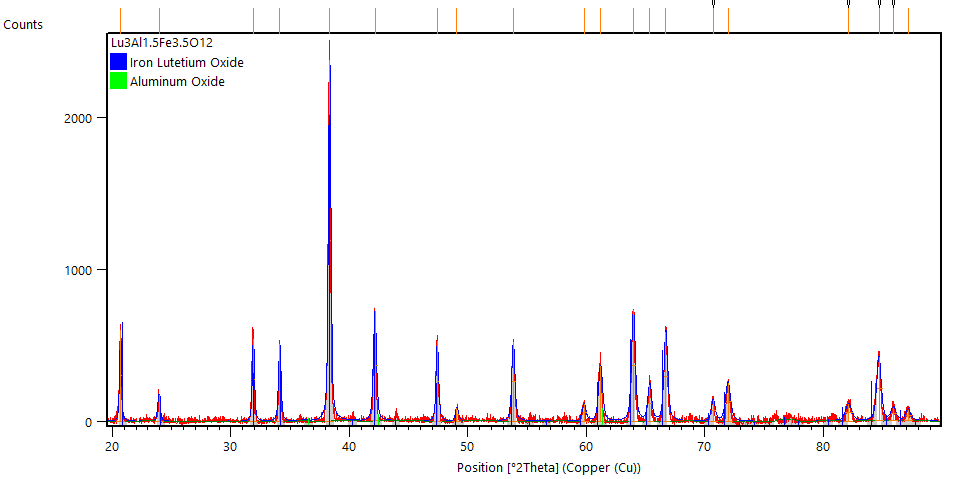
\includegraphics[width=\textwidth]{Anexos/x=35}%
		\caption{Análisis del patrón de difracción de rayos X de la muestra
		\ce{Lu_{3.0}Al_{1.5}Fe_{3.5}O12}} \label{fig:XpertX35}
	\end{figure}

	\begin{figure}[h]
		\centering%
		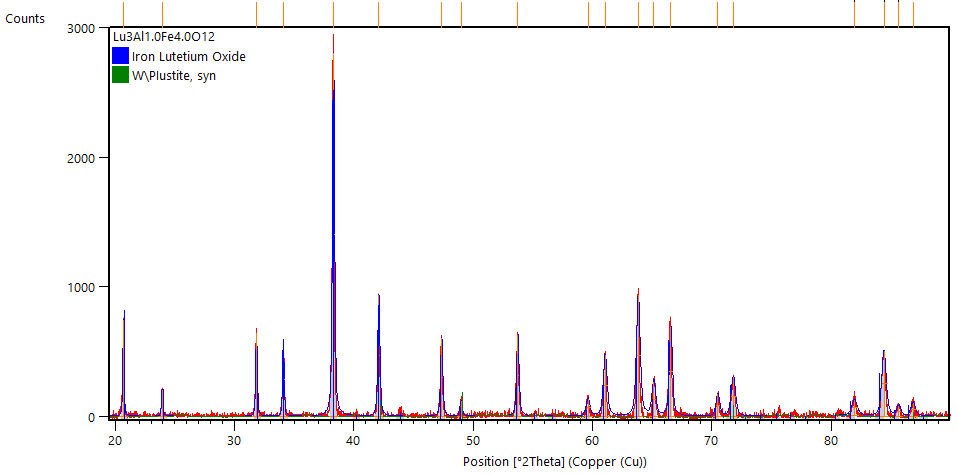
\includegraphics[width=\textwidth]{Anexos/x=40.png}%
		\caption{Análisis del patrón de difracción de rayos X de la muestra
		\ce{Lu_{3.0}Al_{1.0}Fe_{4.0}O12}} \label{fig:XpertX40}
	\end{figure}

	\begin{figure}[t!]
		\centering%
		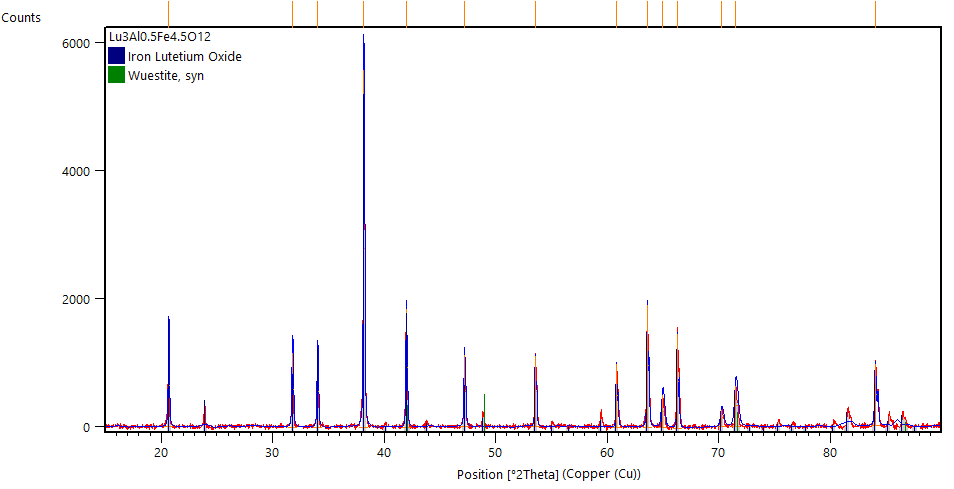
\includegraphics[width=\textwidth]{Anexos/x=45.png}%
		\caption{Análisis del patrón de difracción de rayos X de la muestra
		\ce{Lu_{3.0}Al_{0.5}Fe_{4.5}O12}} \label{fig:XpertX45}
	\end{figure}

	\chapter{Refinamiento Rietveld}\label{AnexoB}

	\begin{figure}[h]
		\centering%
		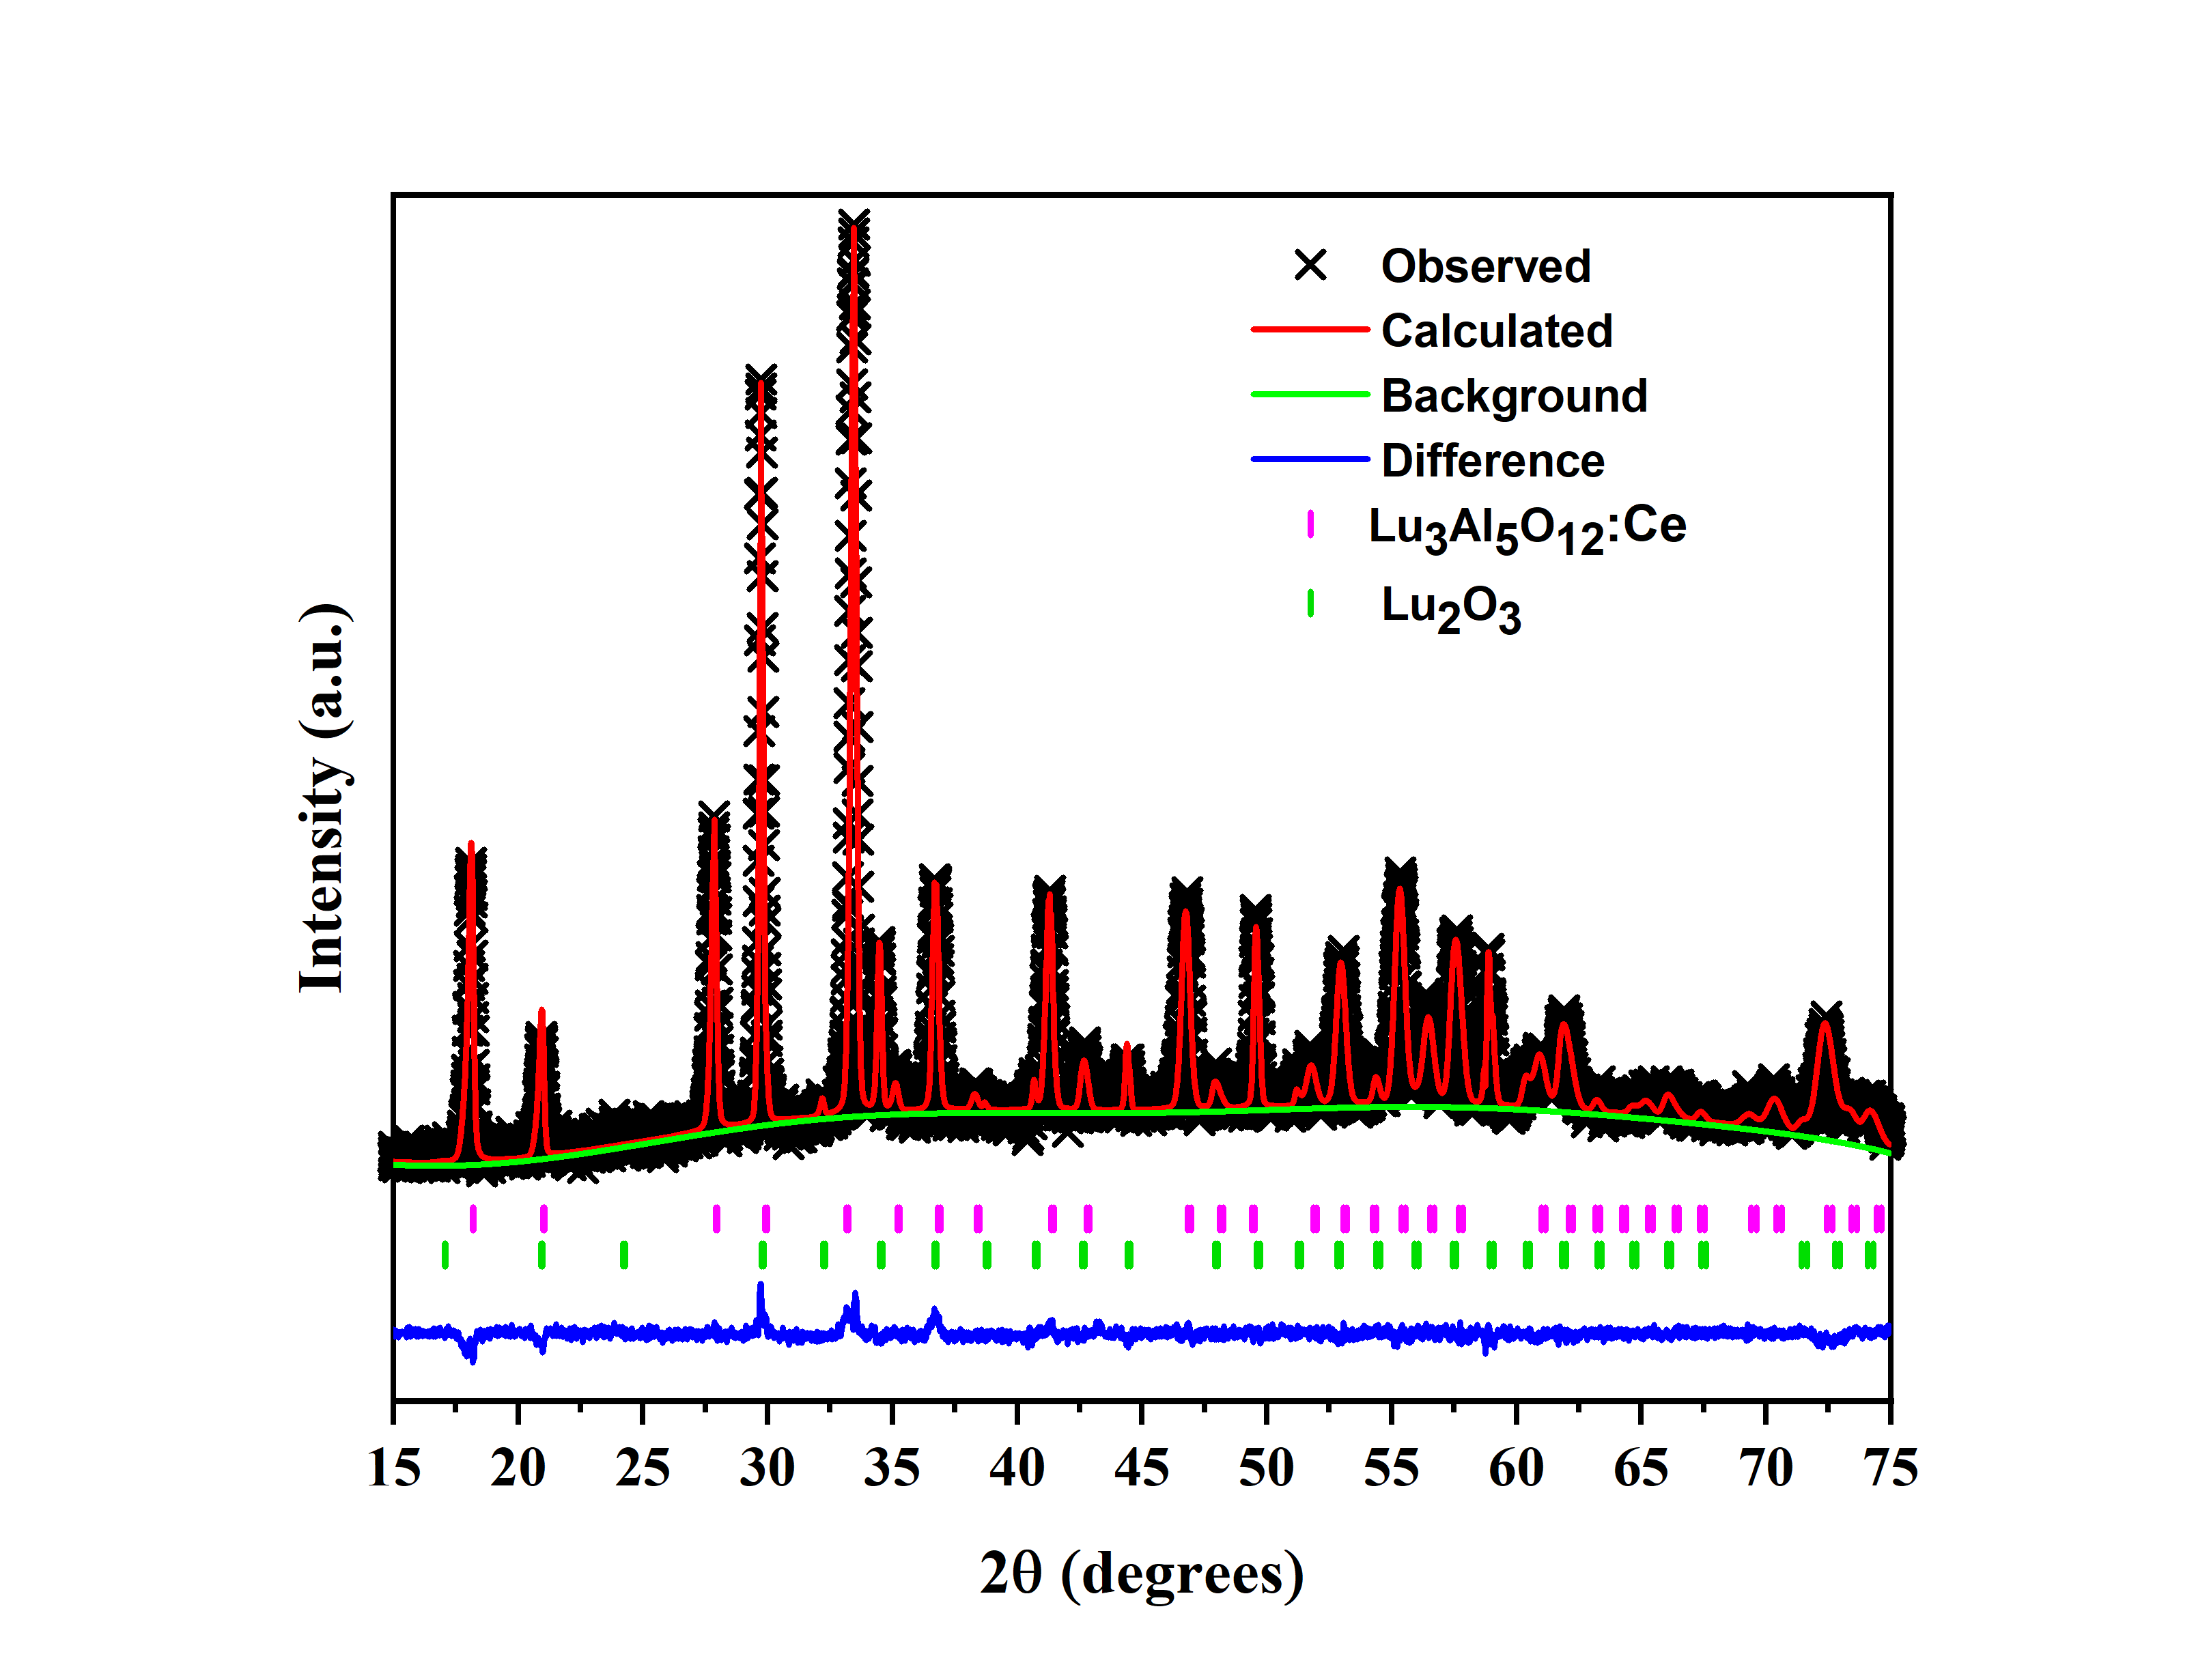
\includegraphics[width=12cm]{Anexos/x00.png}%
		\caption{Resultados de refinamiento Rietveld de a \ce{Lu_{3.0}Al_{5.0}O12}}
		\label{fig:Refi00}
	\end{figure}

	\begin{figure}[h]
		\centering%
		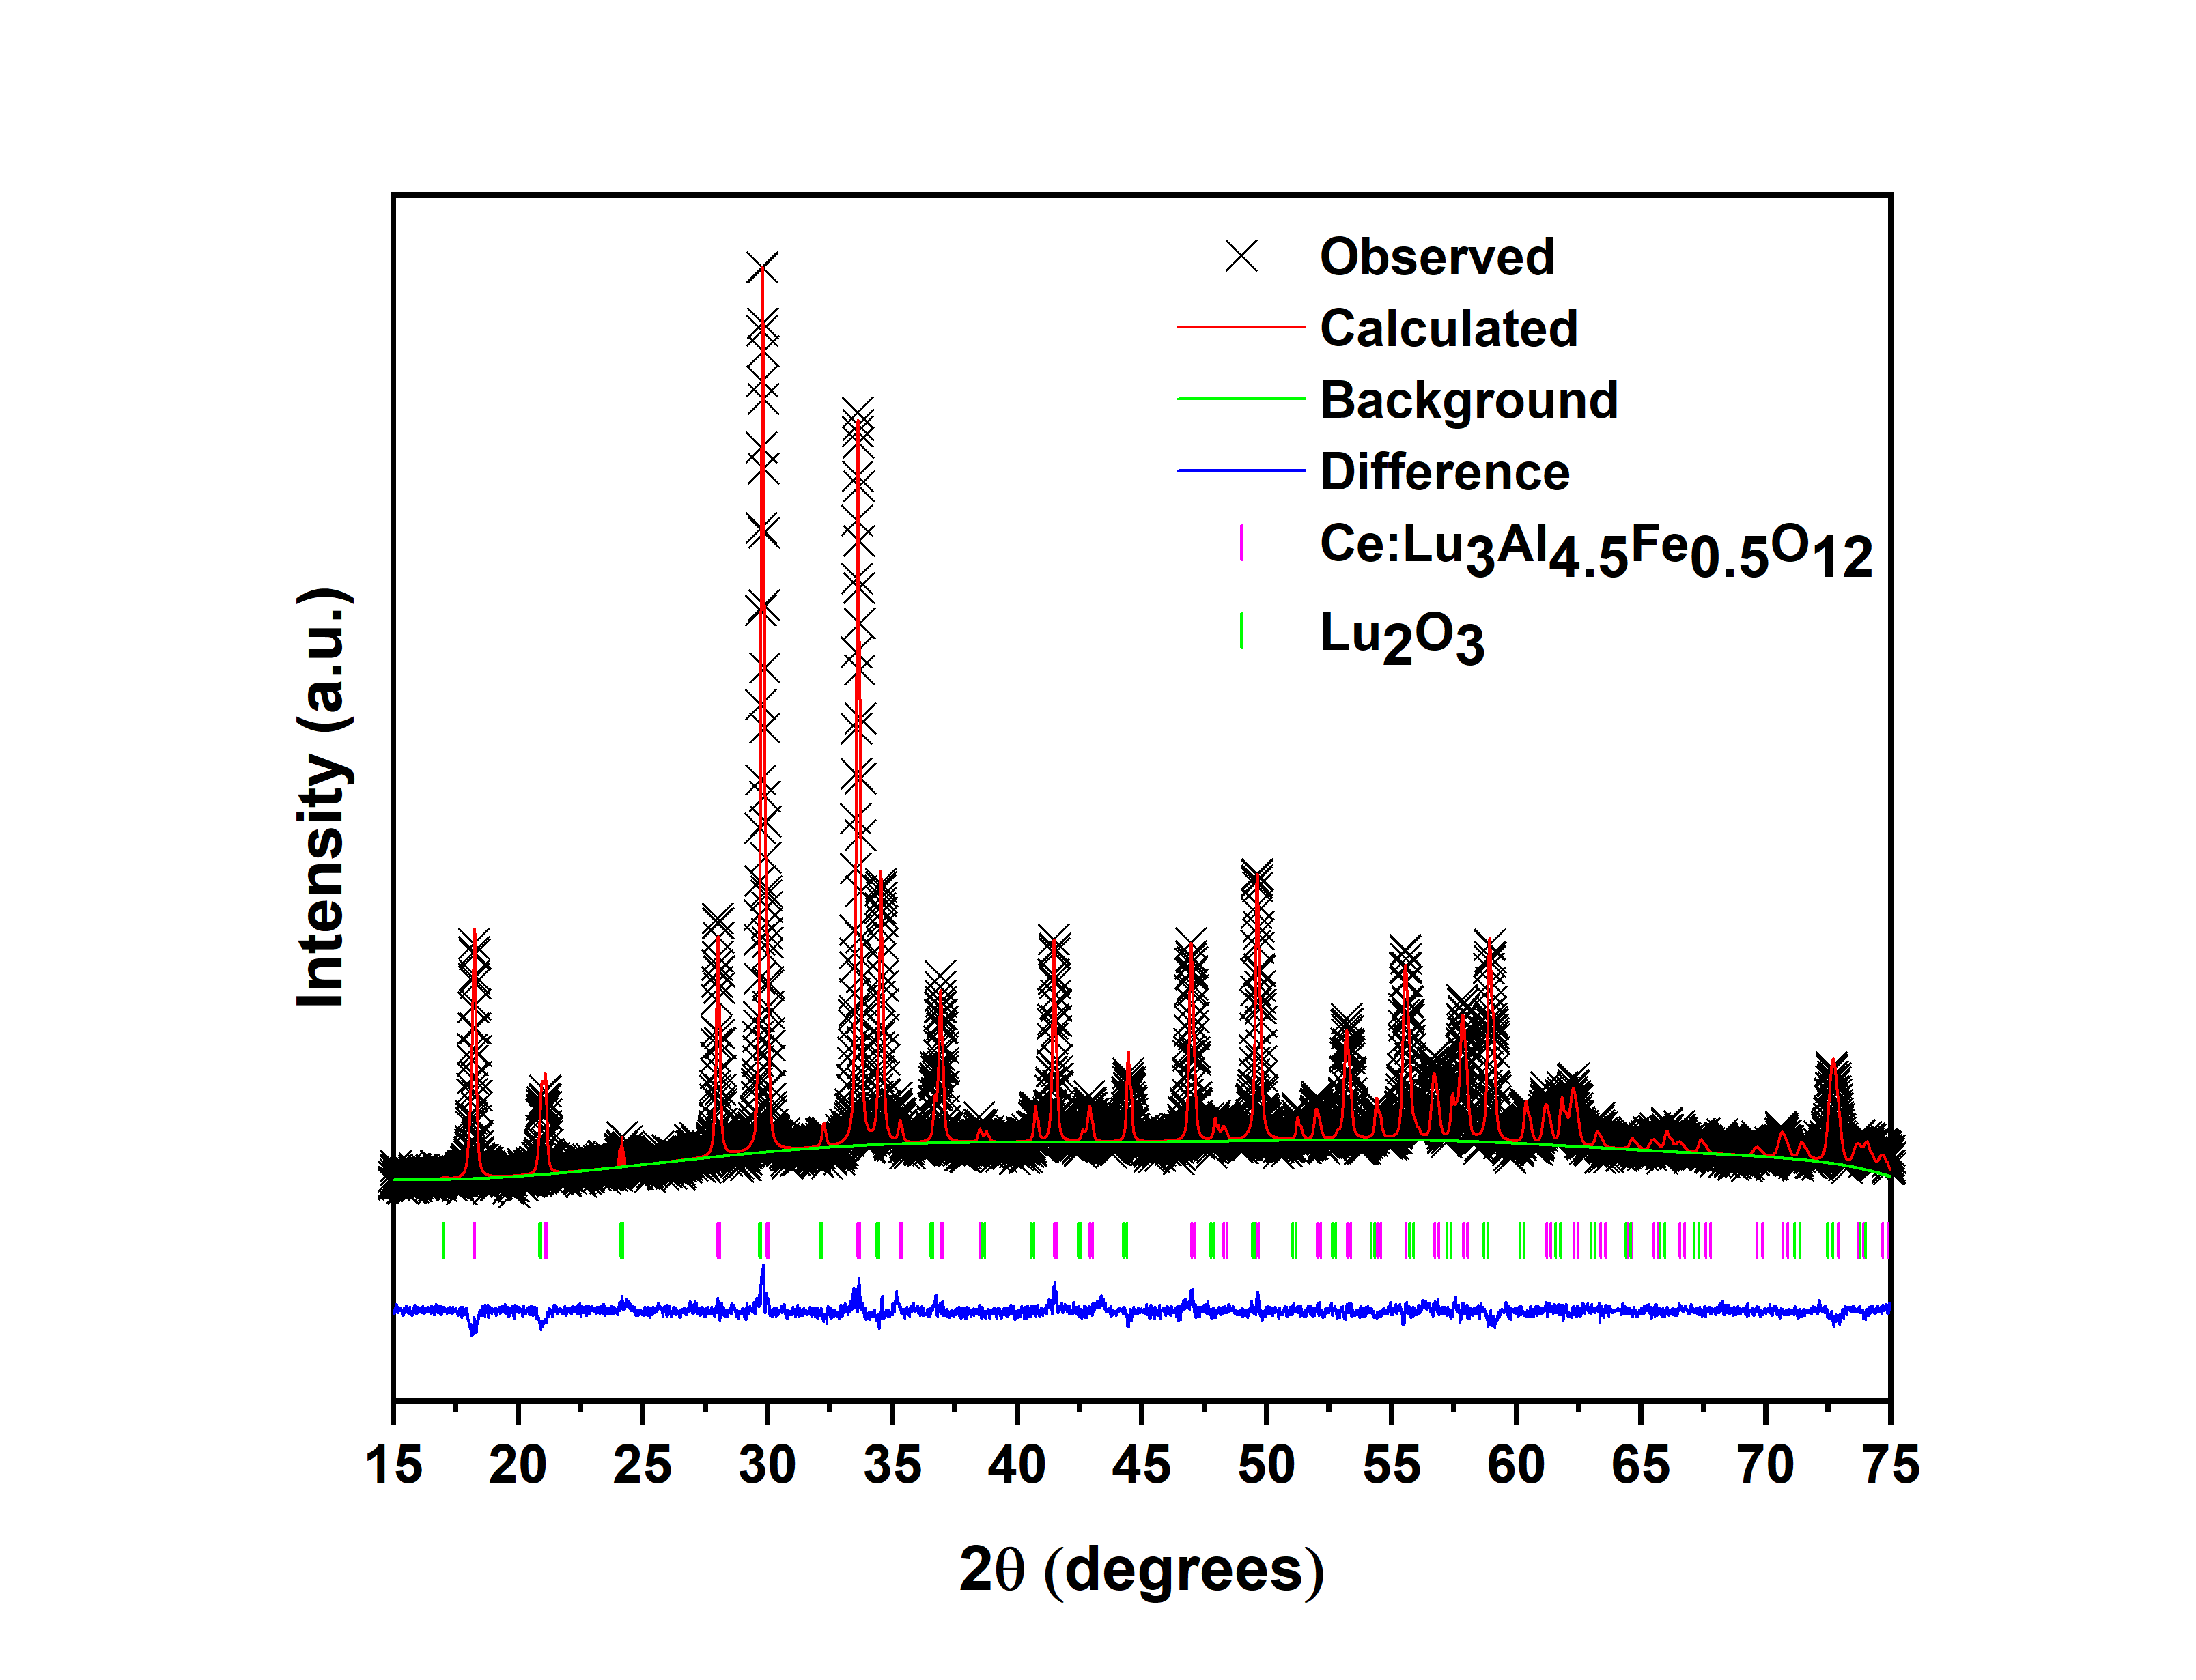
\includegraphics[width=11cm]{Anexos/x05.png}%
		\caption{Resultados de refinamiento Rietveld de
		\ce{Lu_{3.0}Al_{4.5}Fe_{0.5}O12}} \label{fig:refi05}
	\end{figure}

	\begin{figure}[h]
		\centering%
		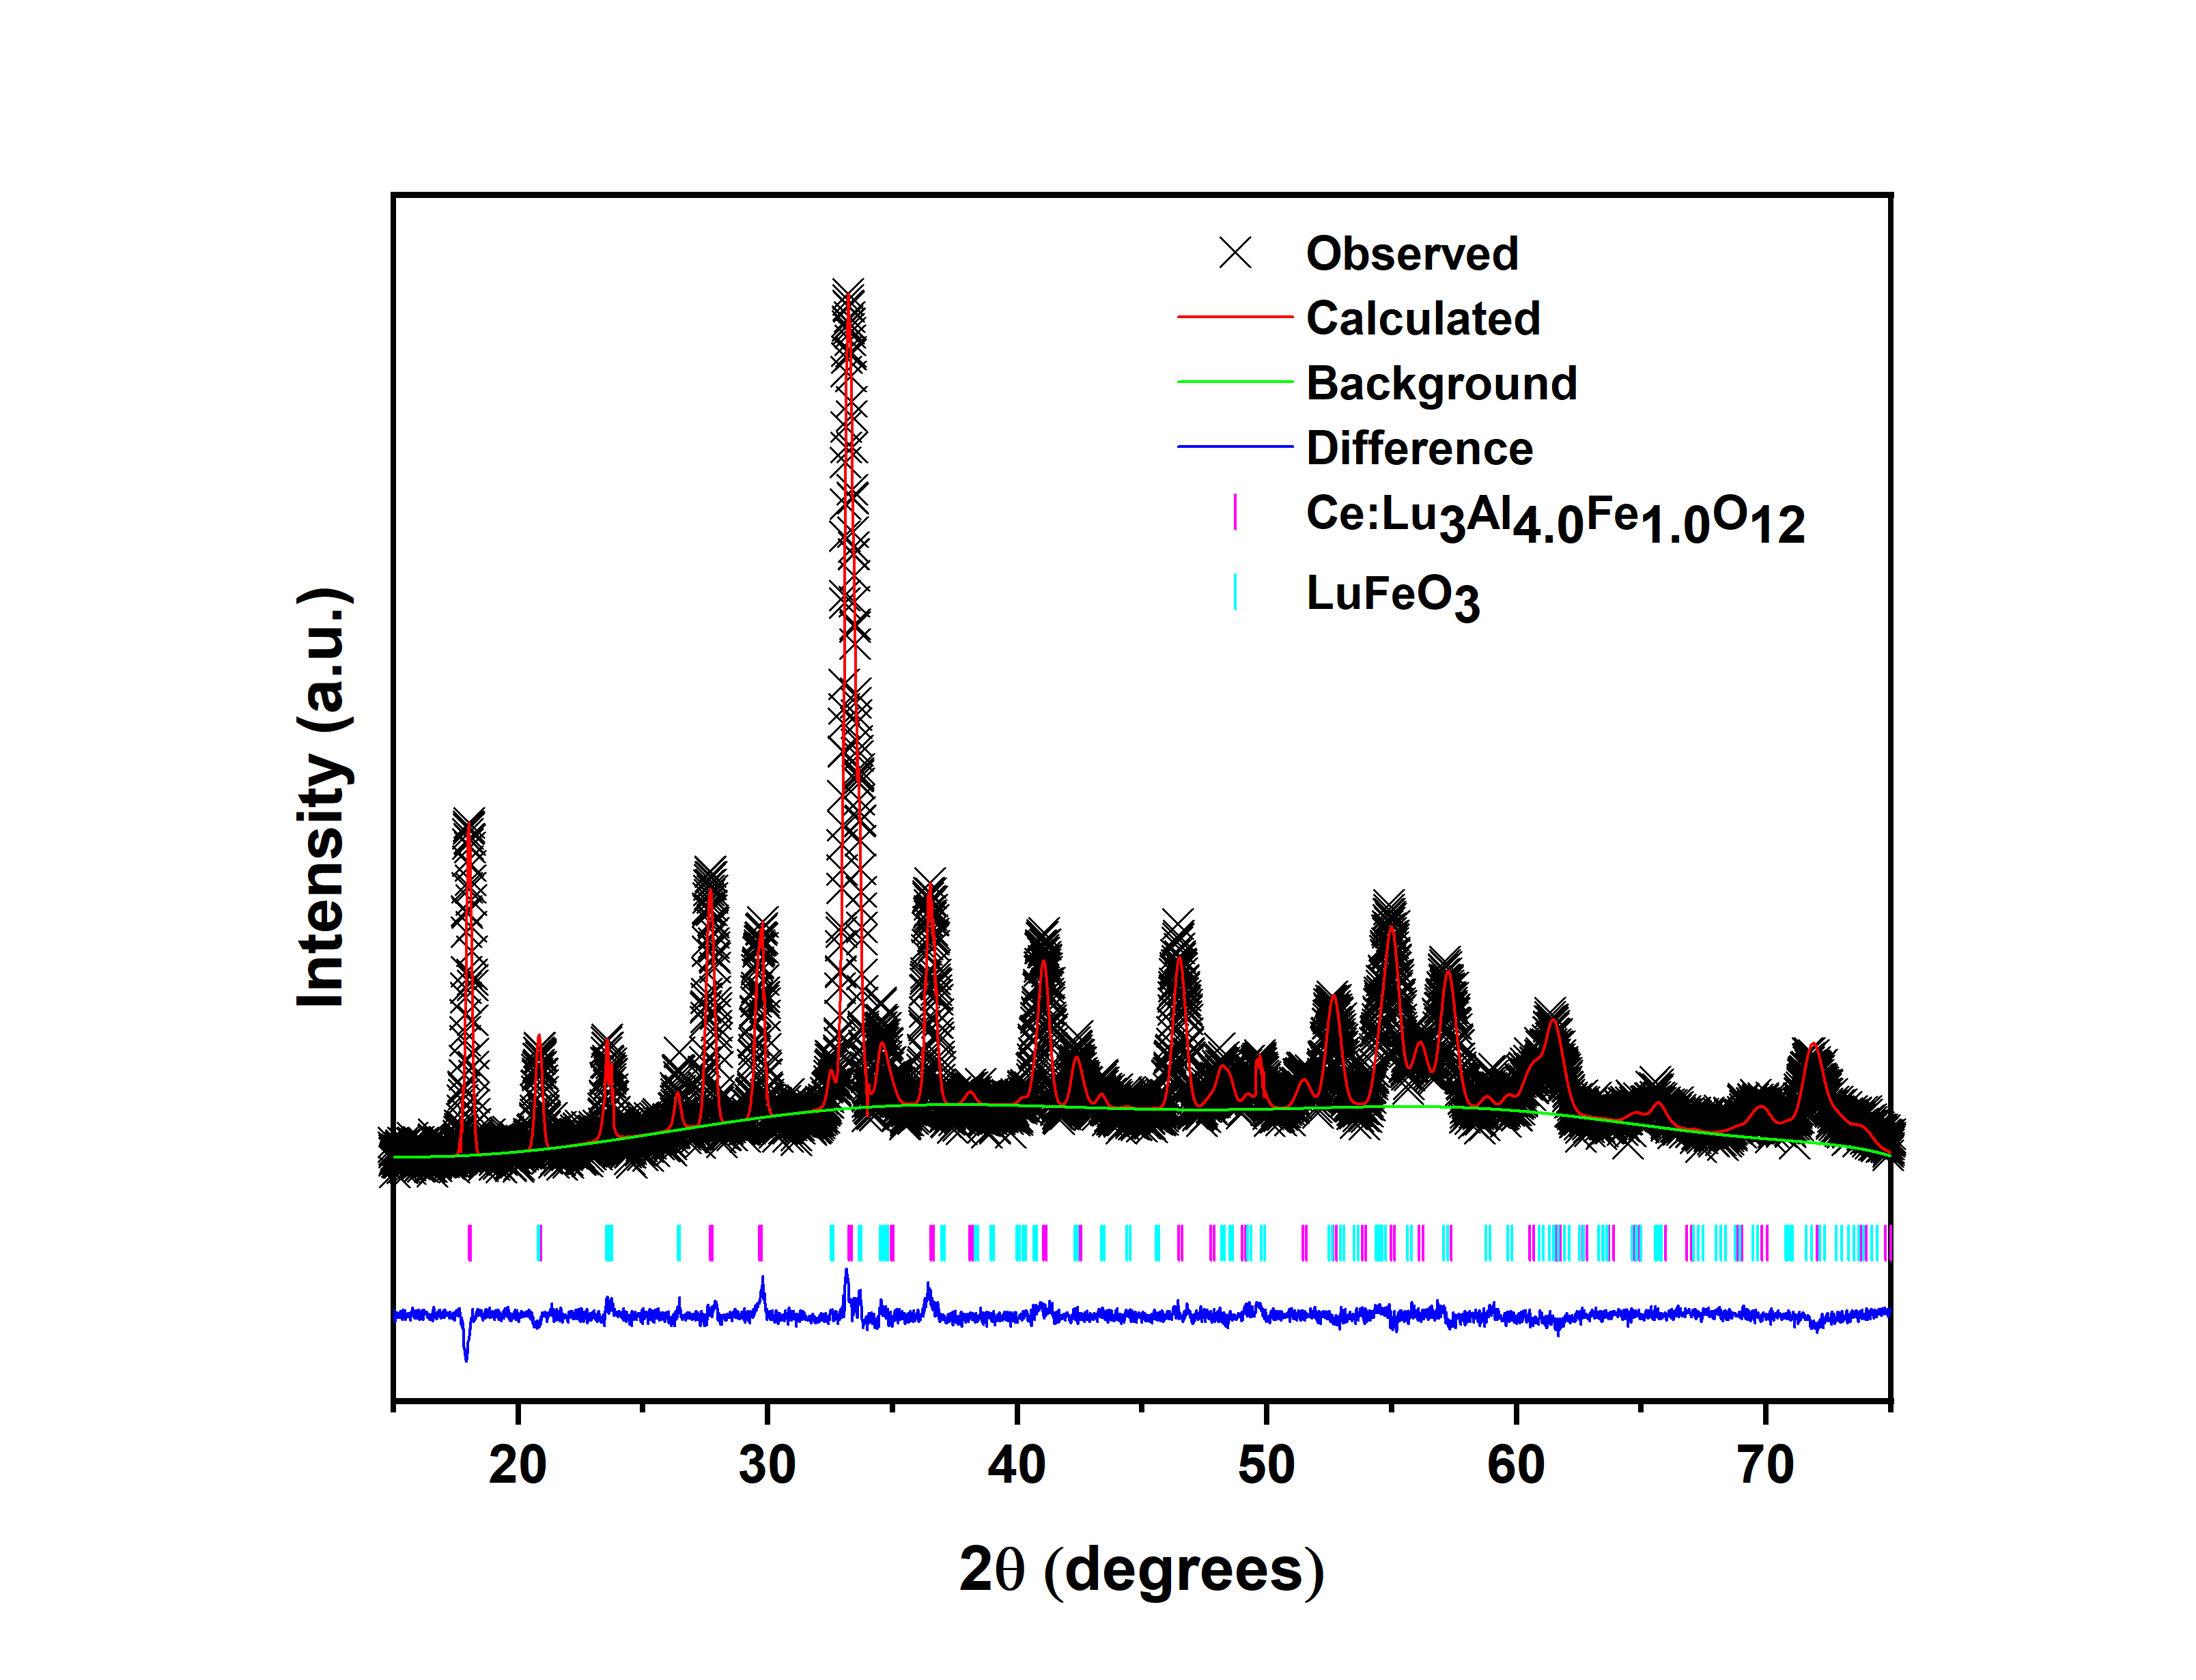
\includegraphics[width=11cm]{Anexos/x10.png}%
		\caption{Resultados de refinamiento Rietveld de
		\ce{Lu_{3.0}Al_{4.0}Fe_{1.0}O12}}\label{fig:refi10}
	\end{figure}

	\begin{figure}[h]
		\centering%
		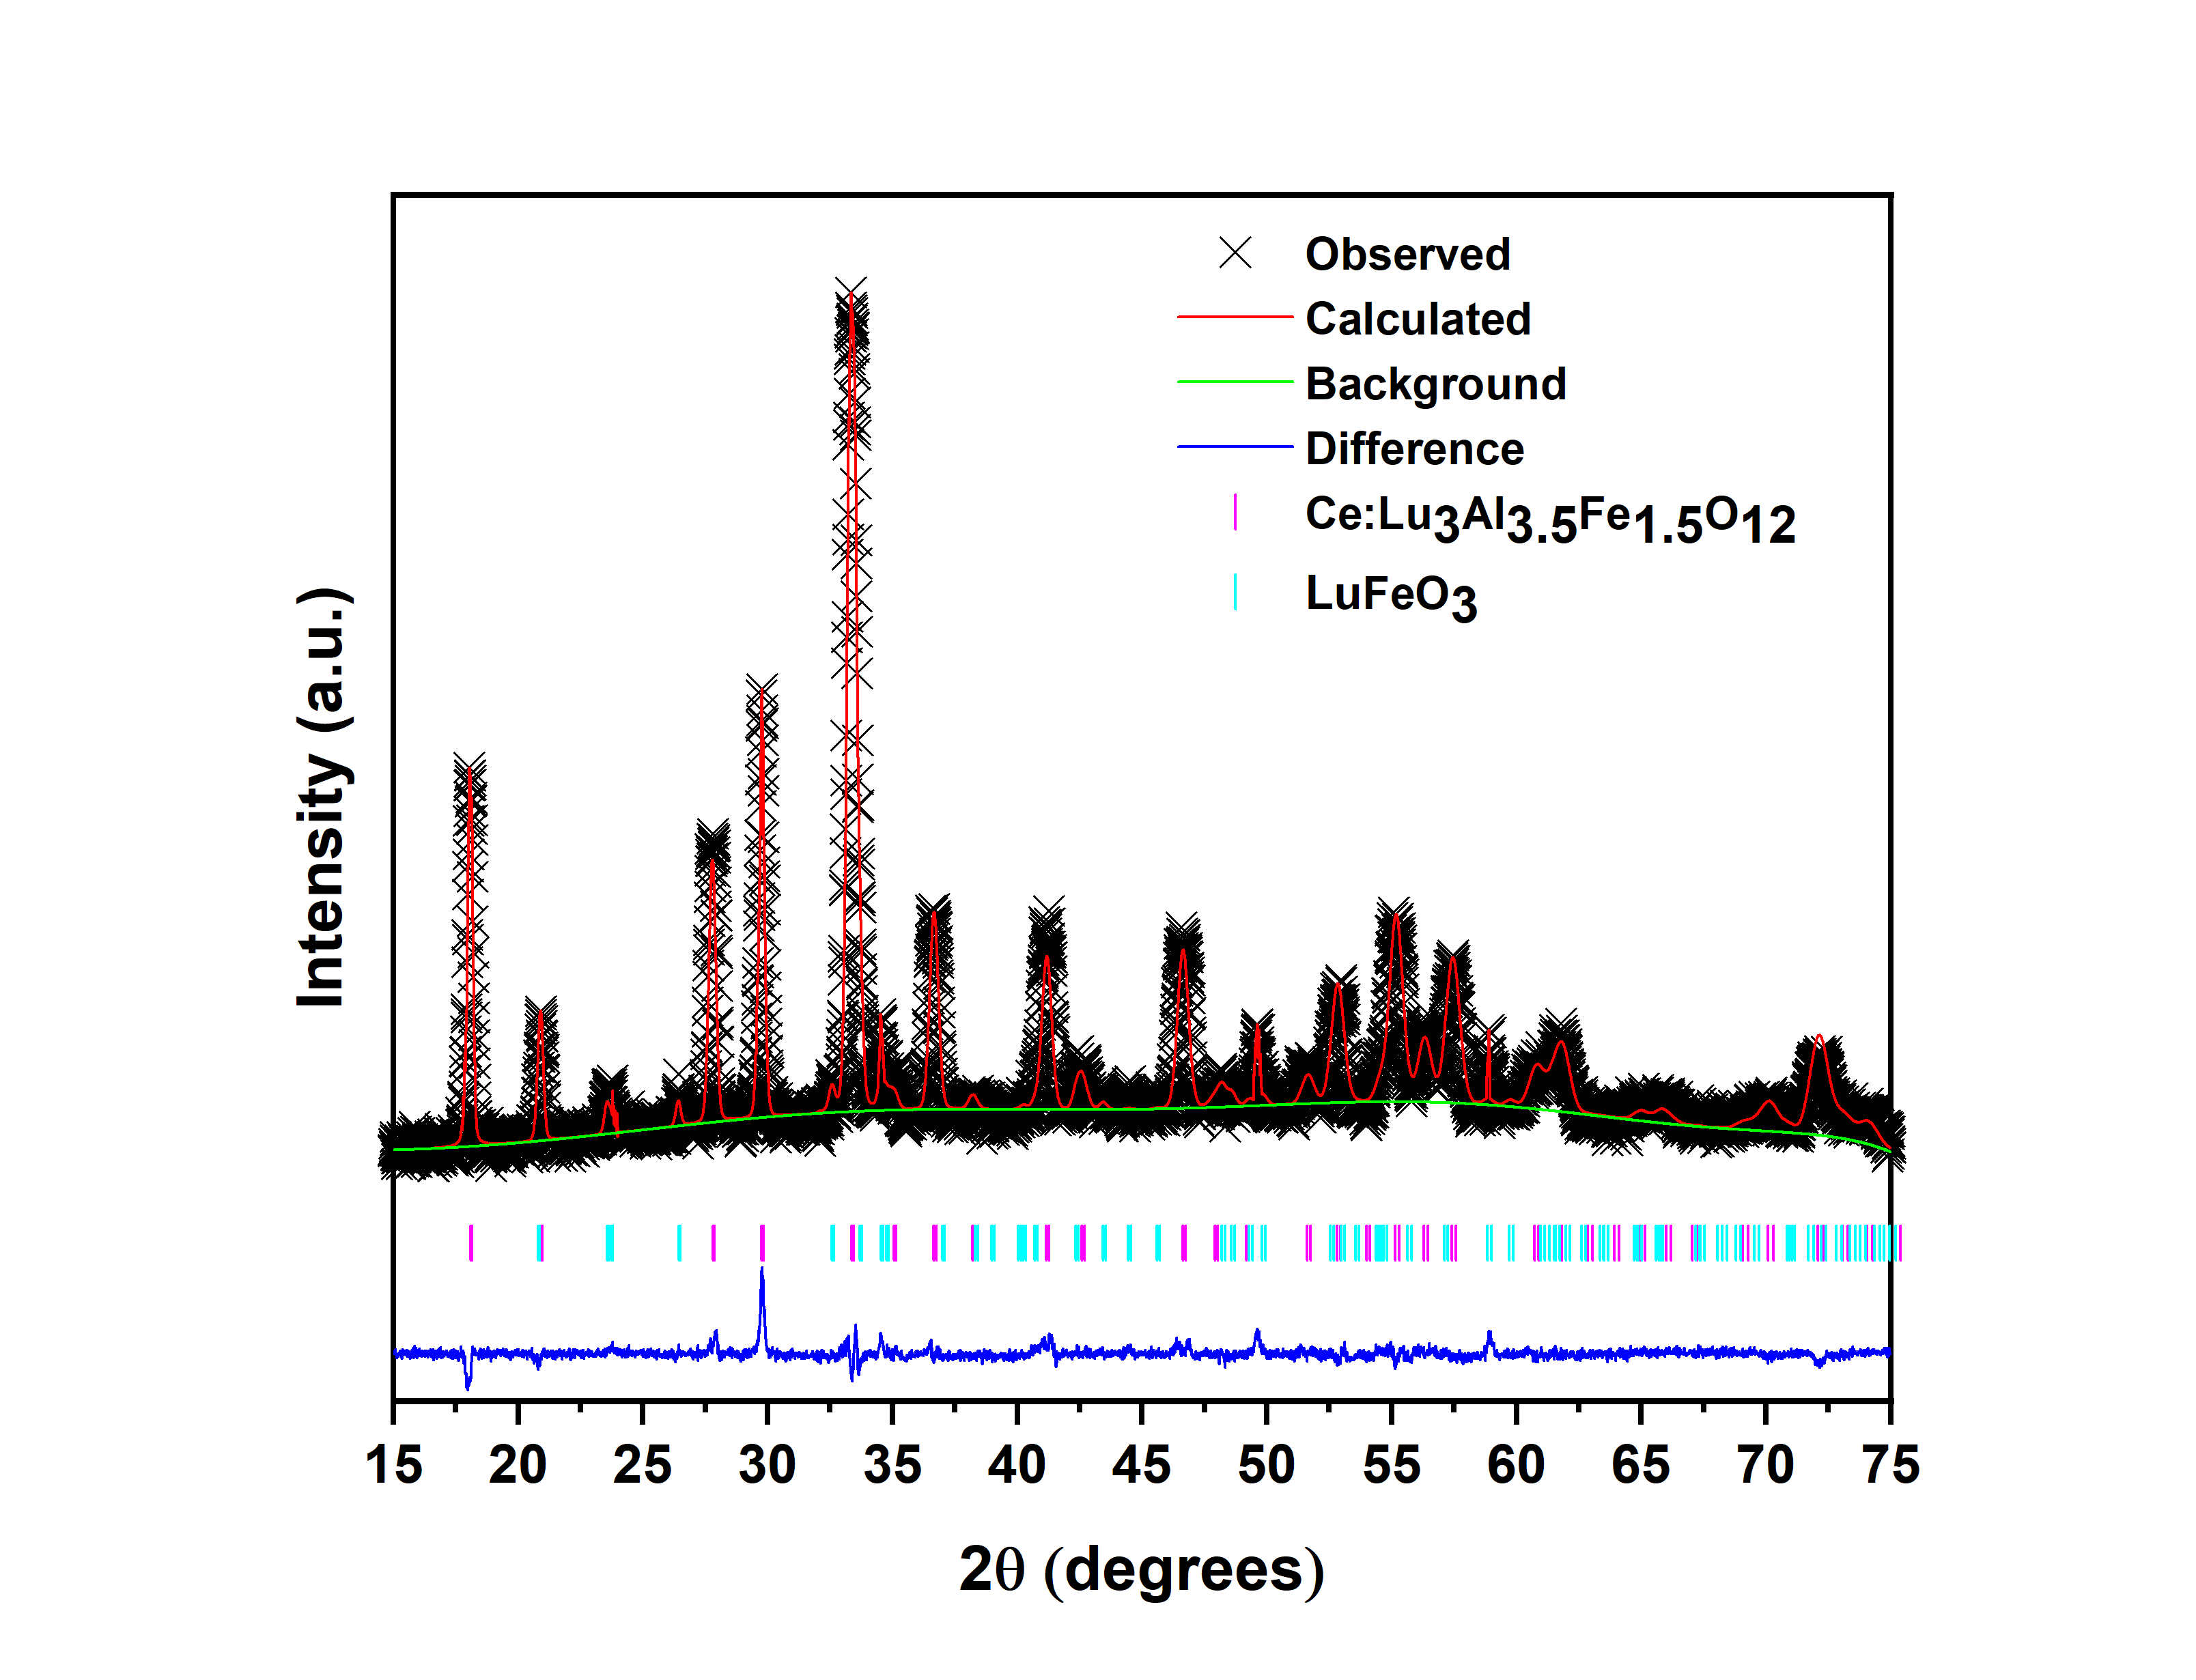
\includegraphics[width=11cm]{Anexos/x15.png}%
		\caption{Resultados de refinamiento Rietveld de
		\ce{Lu_{3.0}Al_{3.5}Fe_{1.5}O12}}\label{fig:refi15}
	\end{figure}

	\begin{figure}[h]
		\centering%
		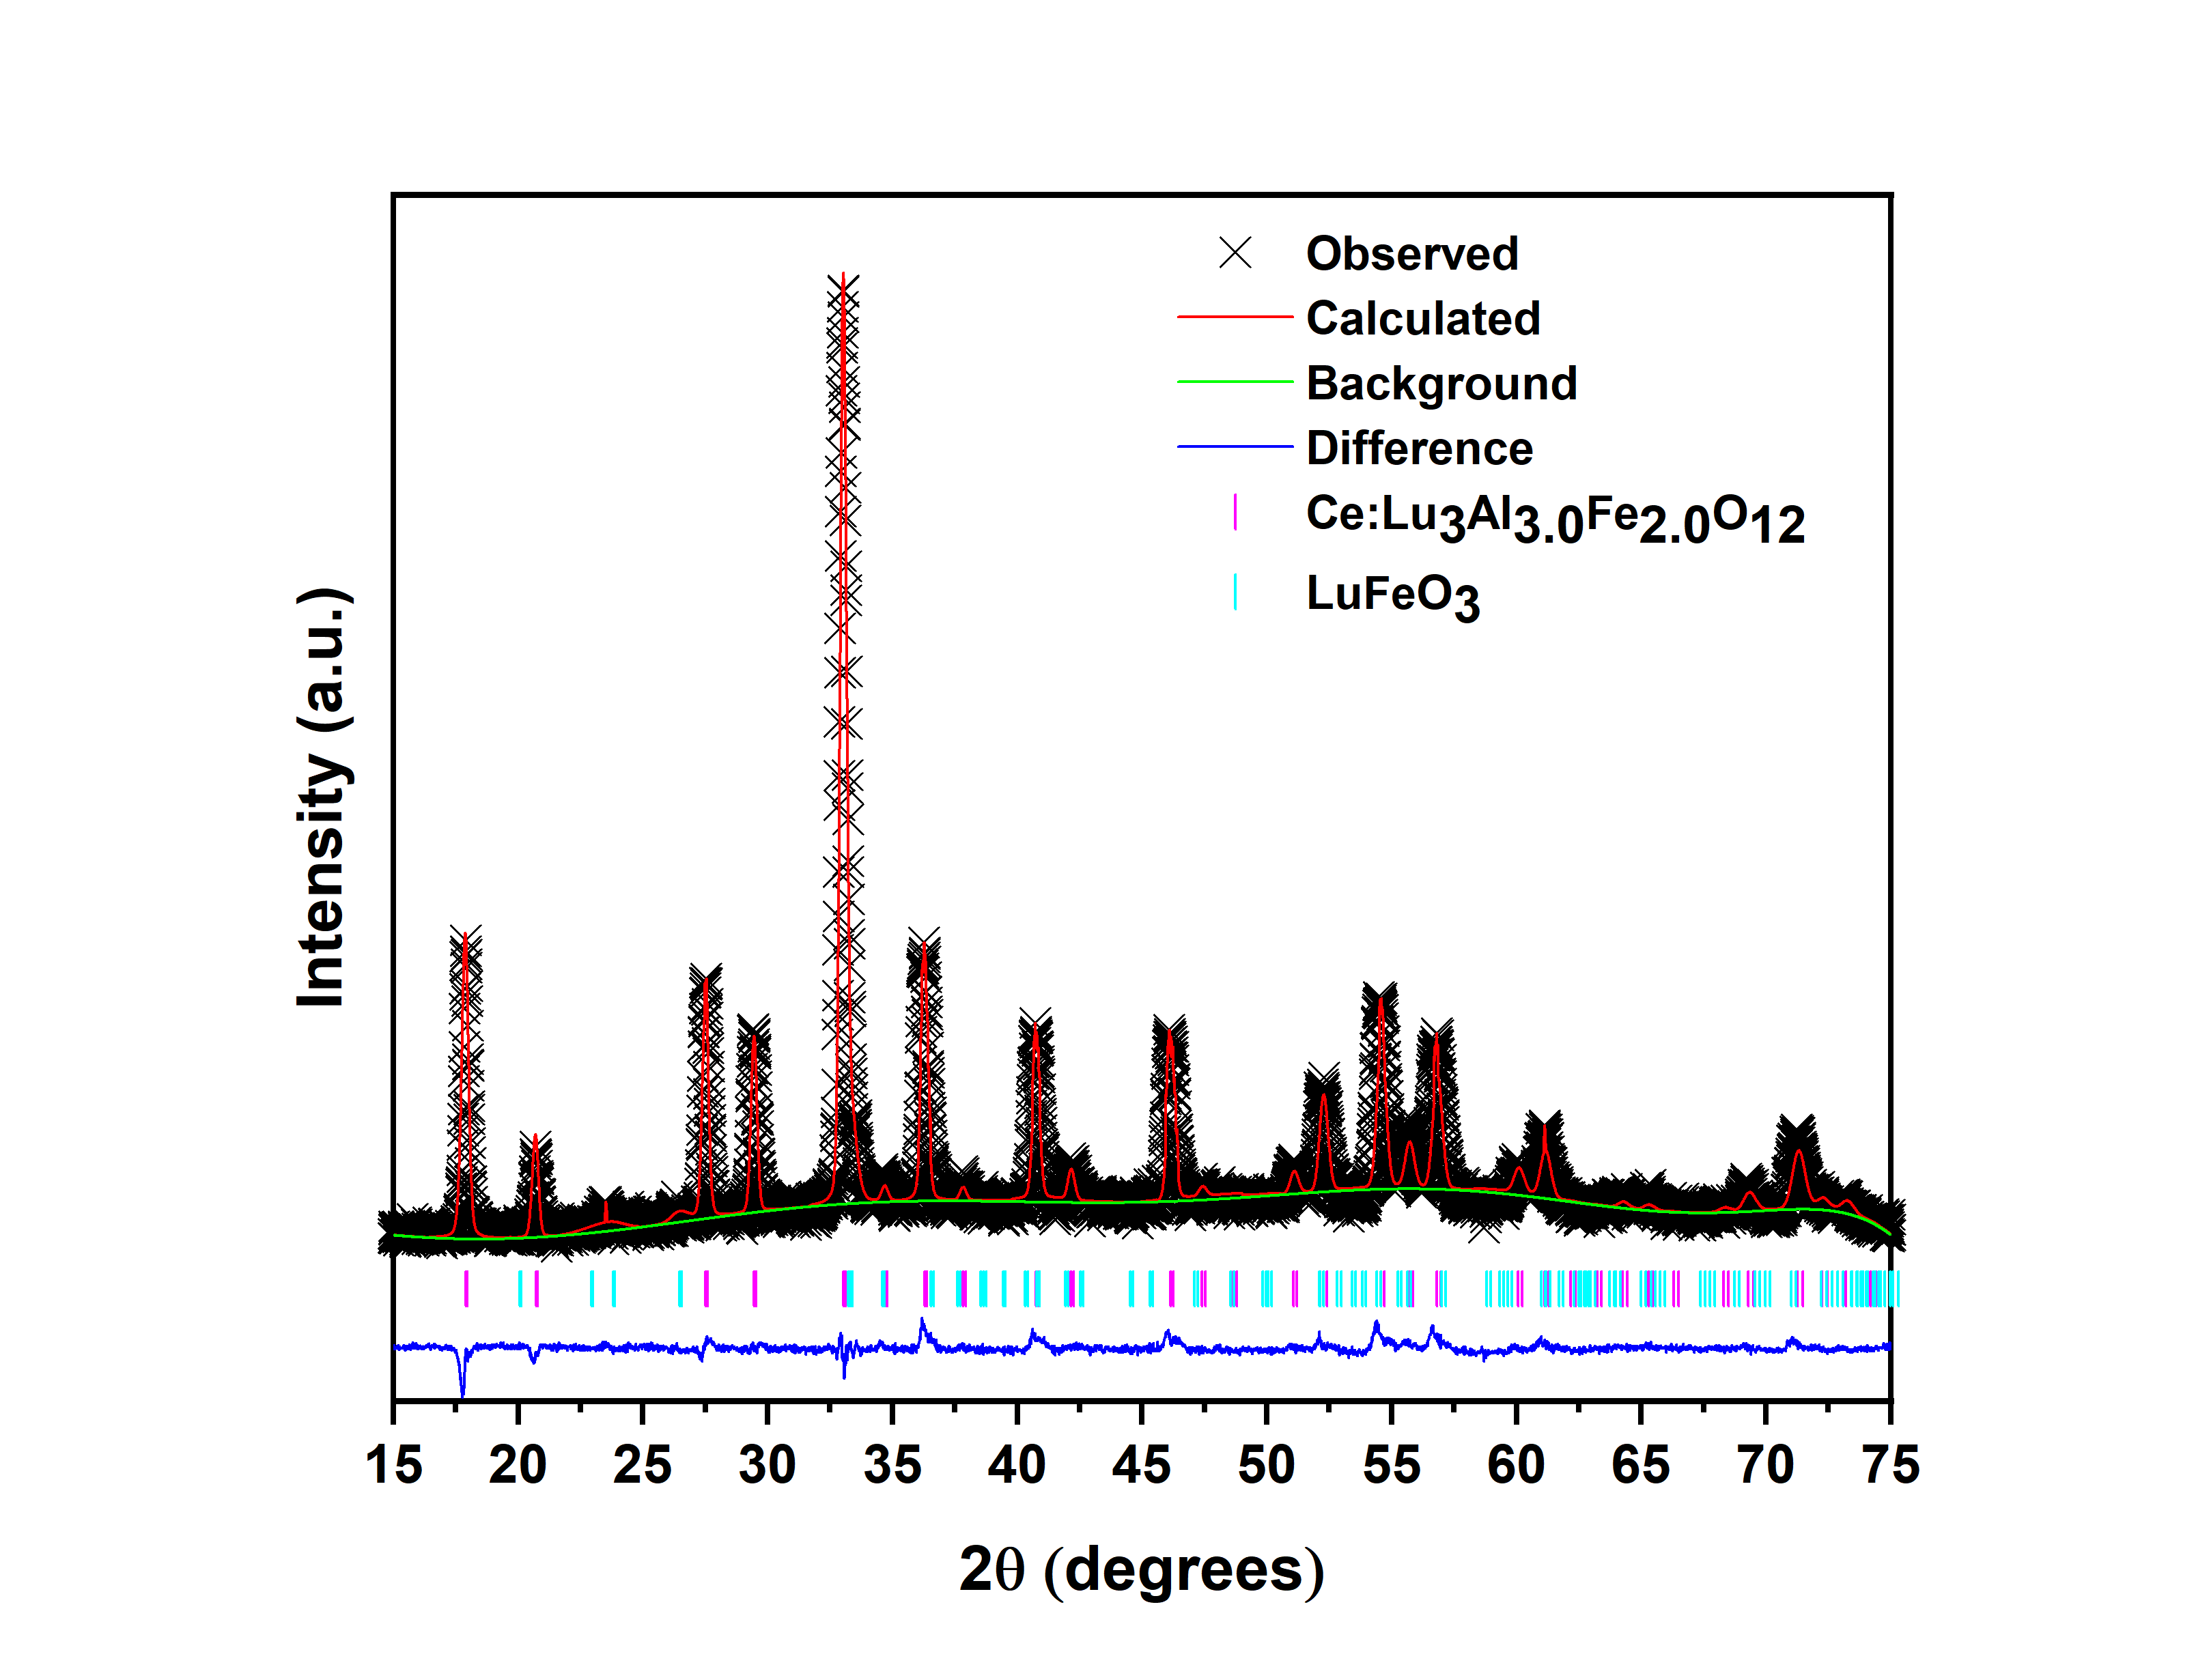
\includegraphics[width=11cm]{Anexos/x20.png}%
		\caption{Resultados de refinamiento Rietveld de
		\ce{Lu_{3.0}Al_{3.0}Fe_{2.0}O12}}\label{fig:refi20}
	\end{figure}

	\begin{figure}[h]
		\centering%
		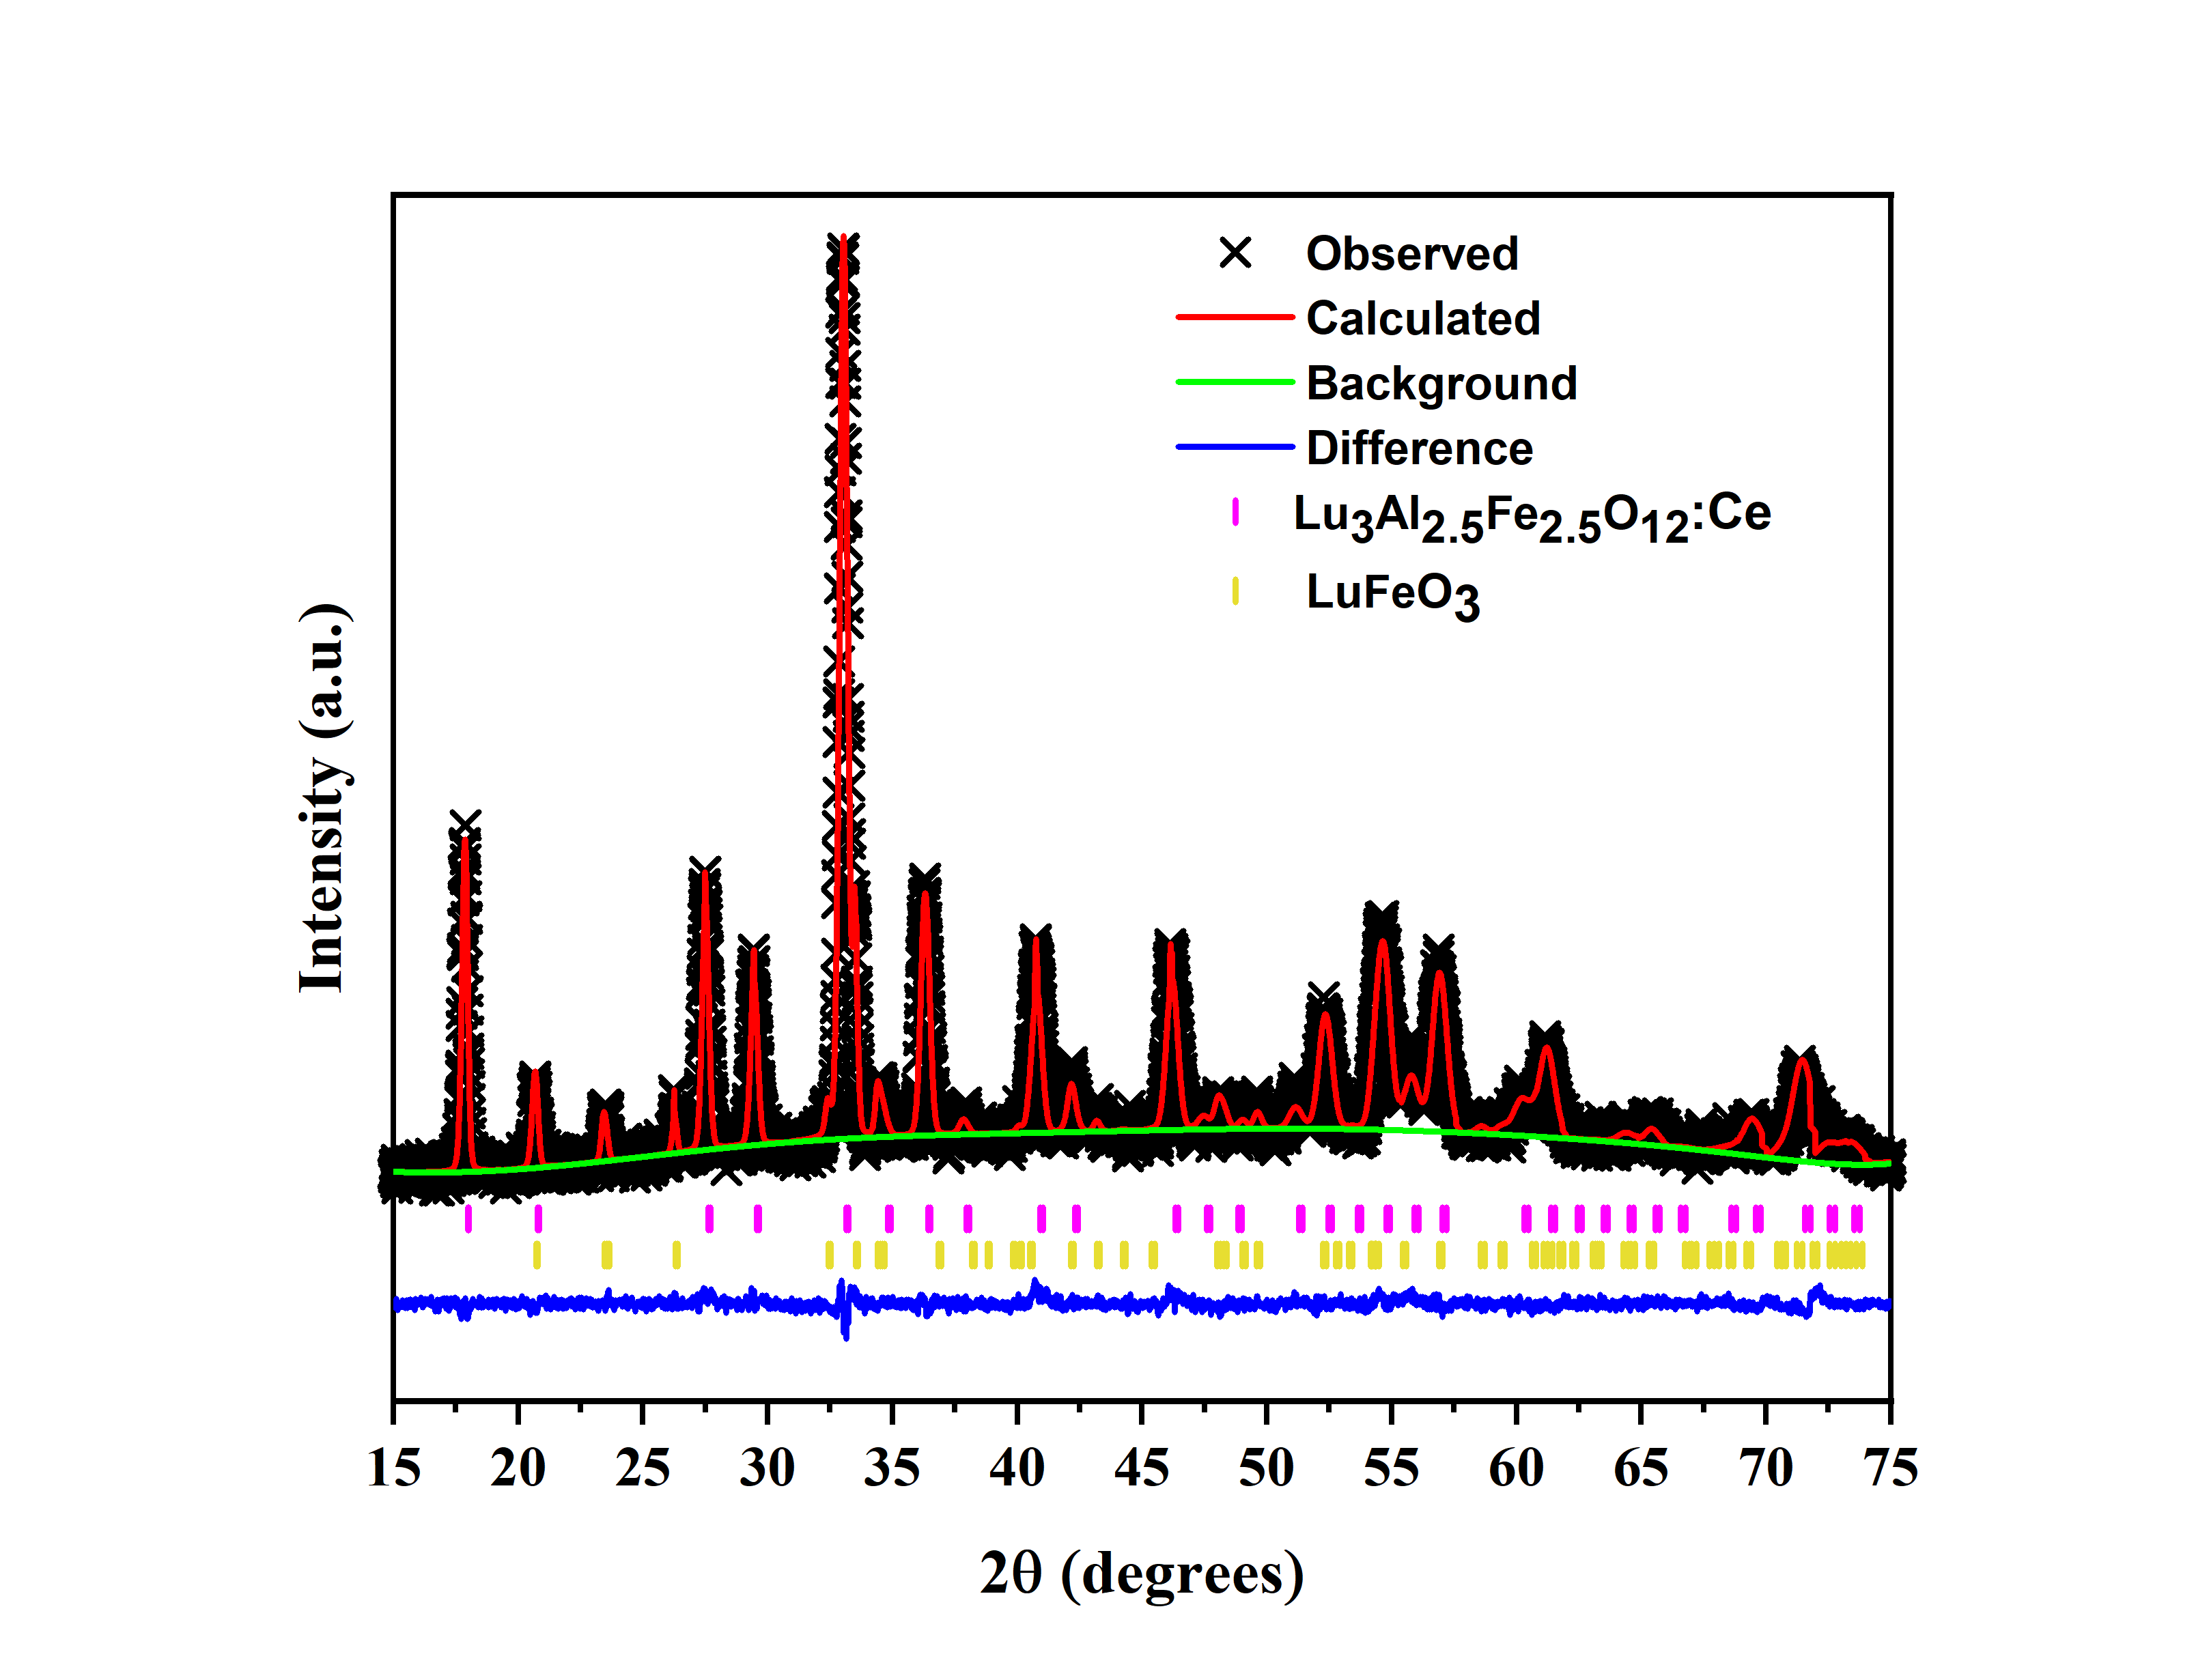
\includegraphics[width=11cm]{Anexos/x25.png}%
		\caption{Resultados de refinamiento Rietveld de
		\ce{Lu_{3.0}Al_{2.5}Fe_{2.5}O12}}\label{fig:refi25}
	\end{figure}

	\begin{figure}[h]
		\centering%
		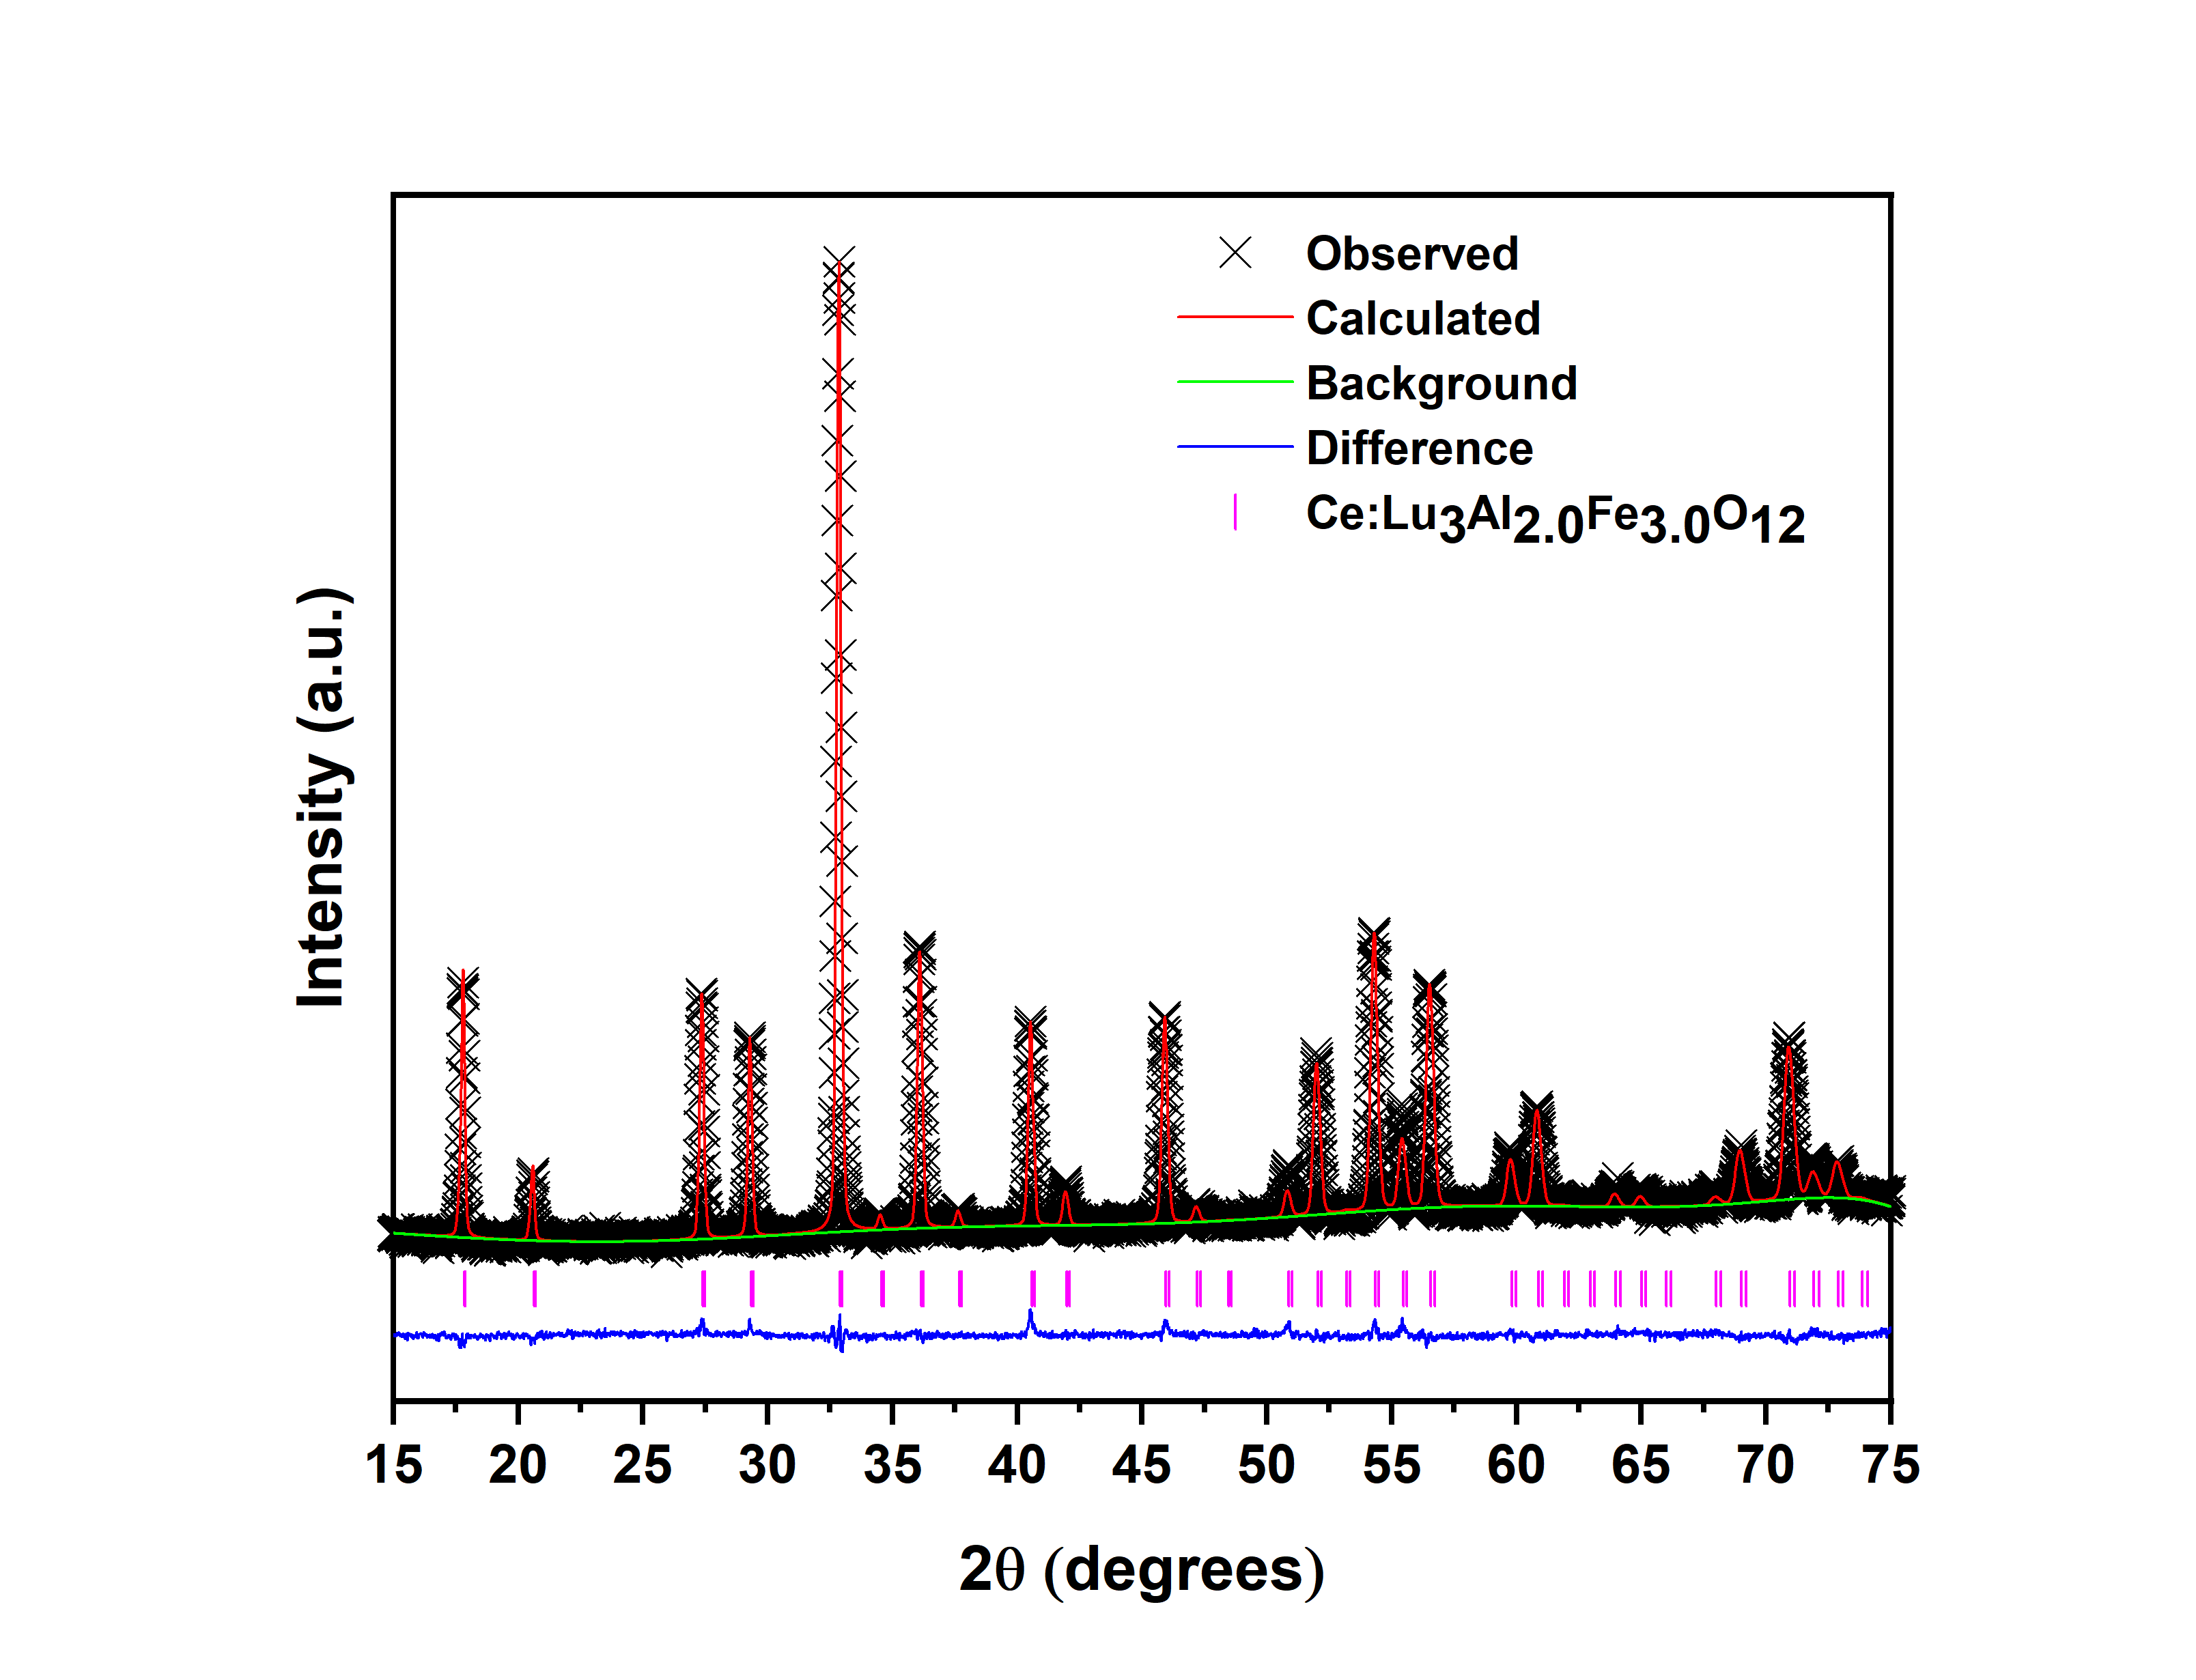
\includegraphics[width=11cm]{Anexos/x30.png}%
		\caption{Resultados de refinamiento Rietveld de
		\ce{Lu_{3.0}Al_{2.0}Fe_{3.0}O12}}\label{fig:refi30}
	\end{figure}

	\begin{figure}[h]
		\centering%
		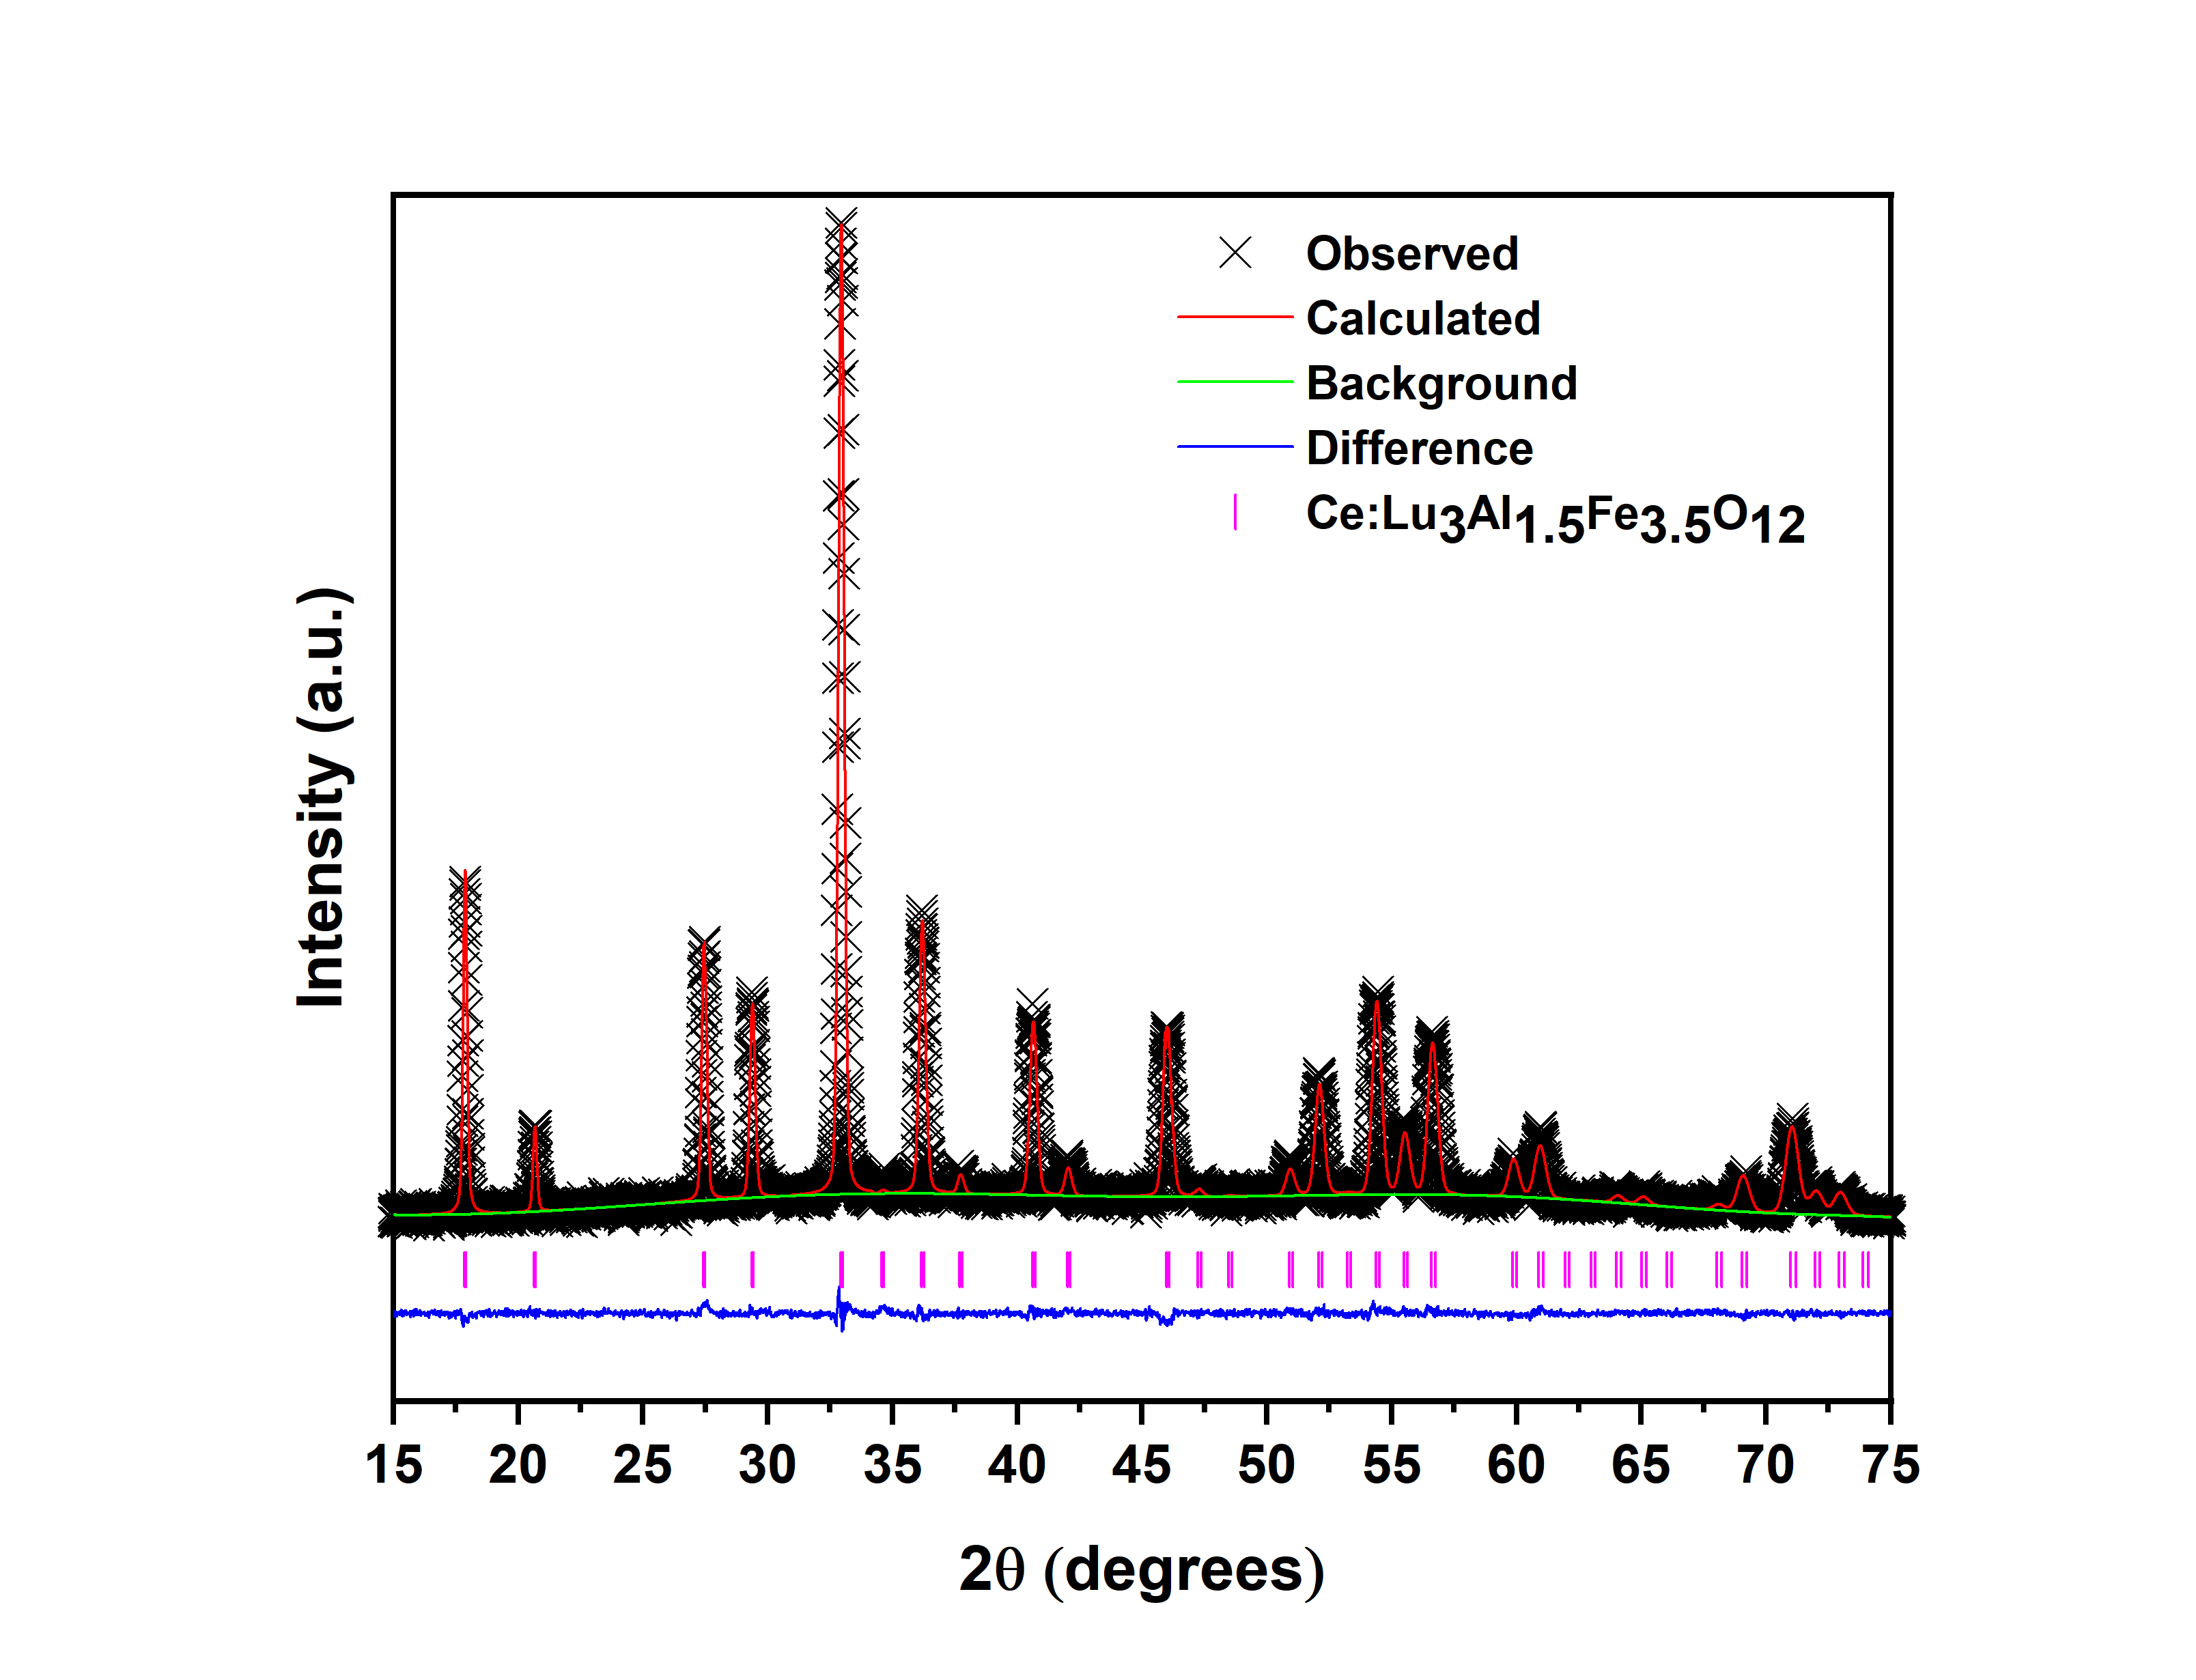
\includegraphics[width=11cm]{Anexos/x35.png}%
		\caption{Resultados de refinamiento Rietveld de
		\ce{Lu_{3.0}Al_{1.5}Fe_{3.5}O12}}\label{fig:refi35}
	\end{figure}

	\begin{figure}[h]
		\centering%
		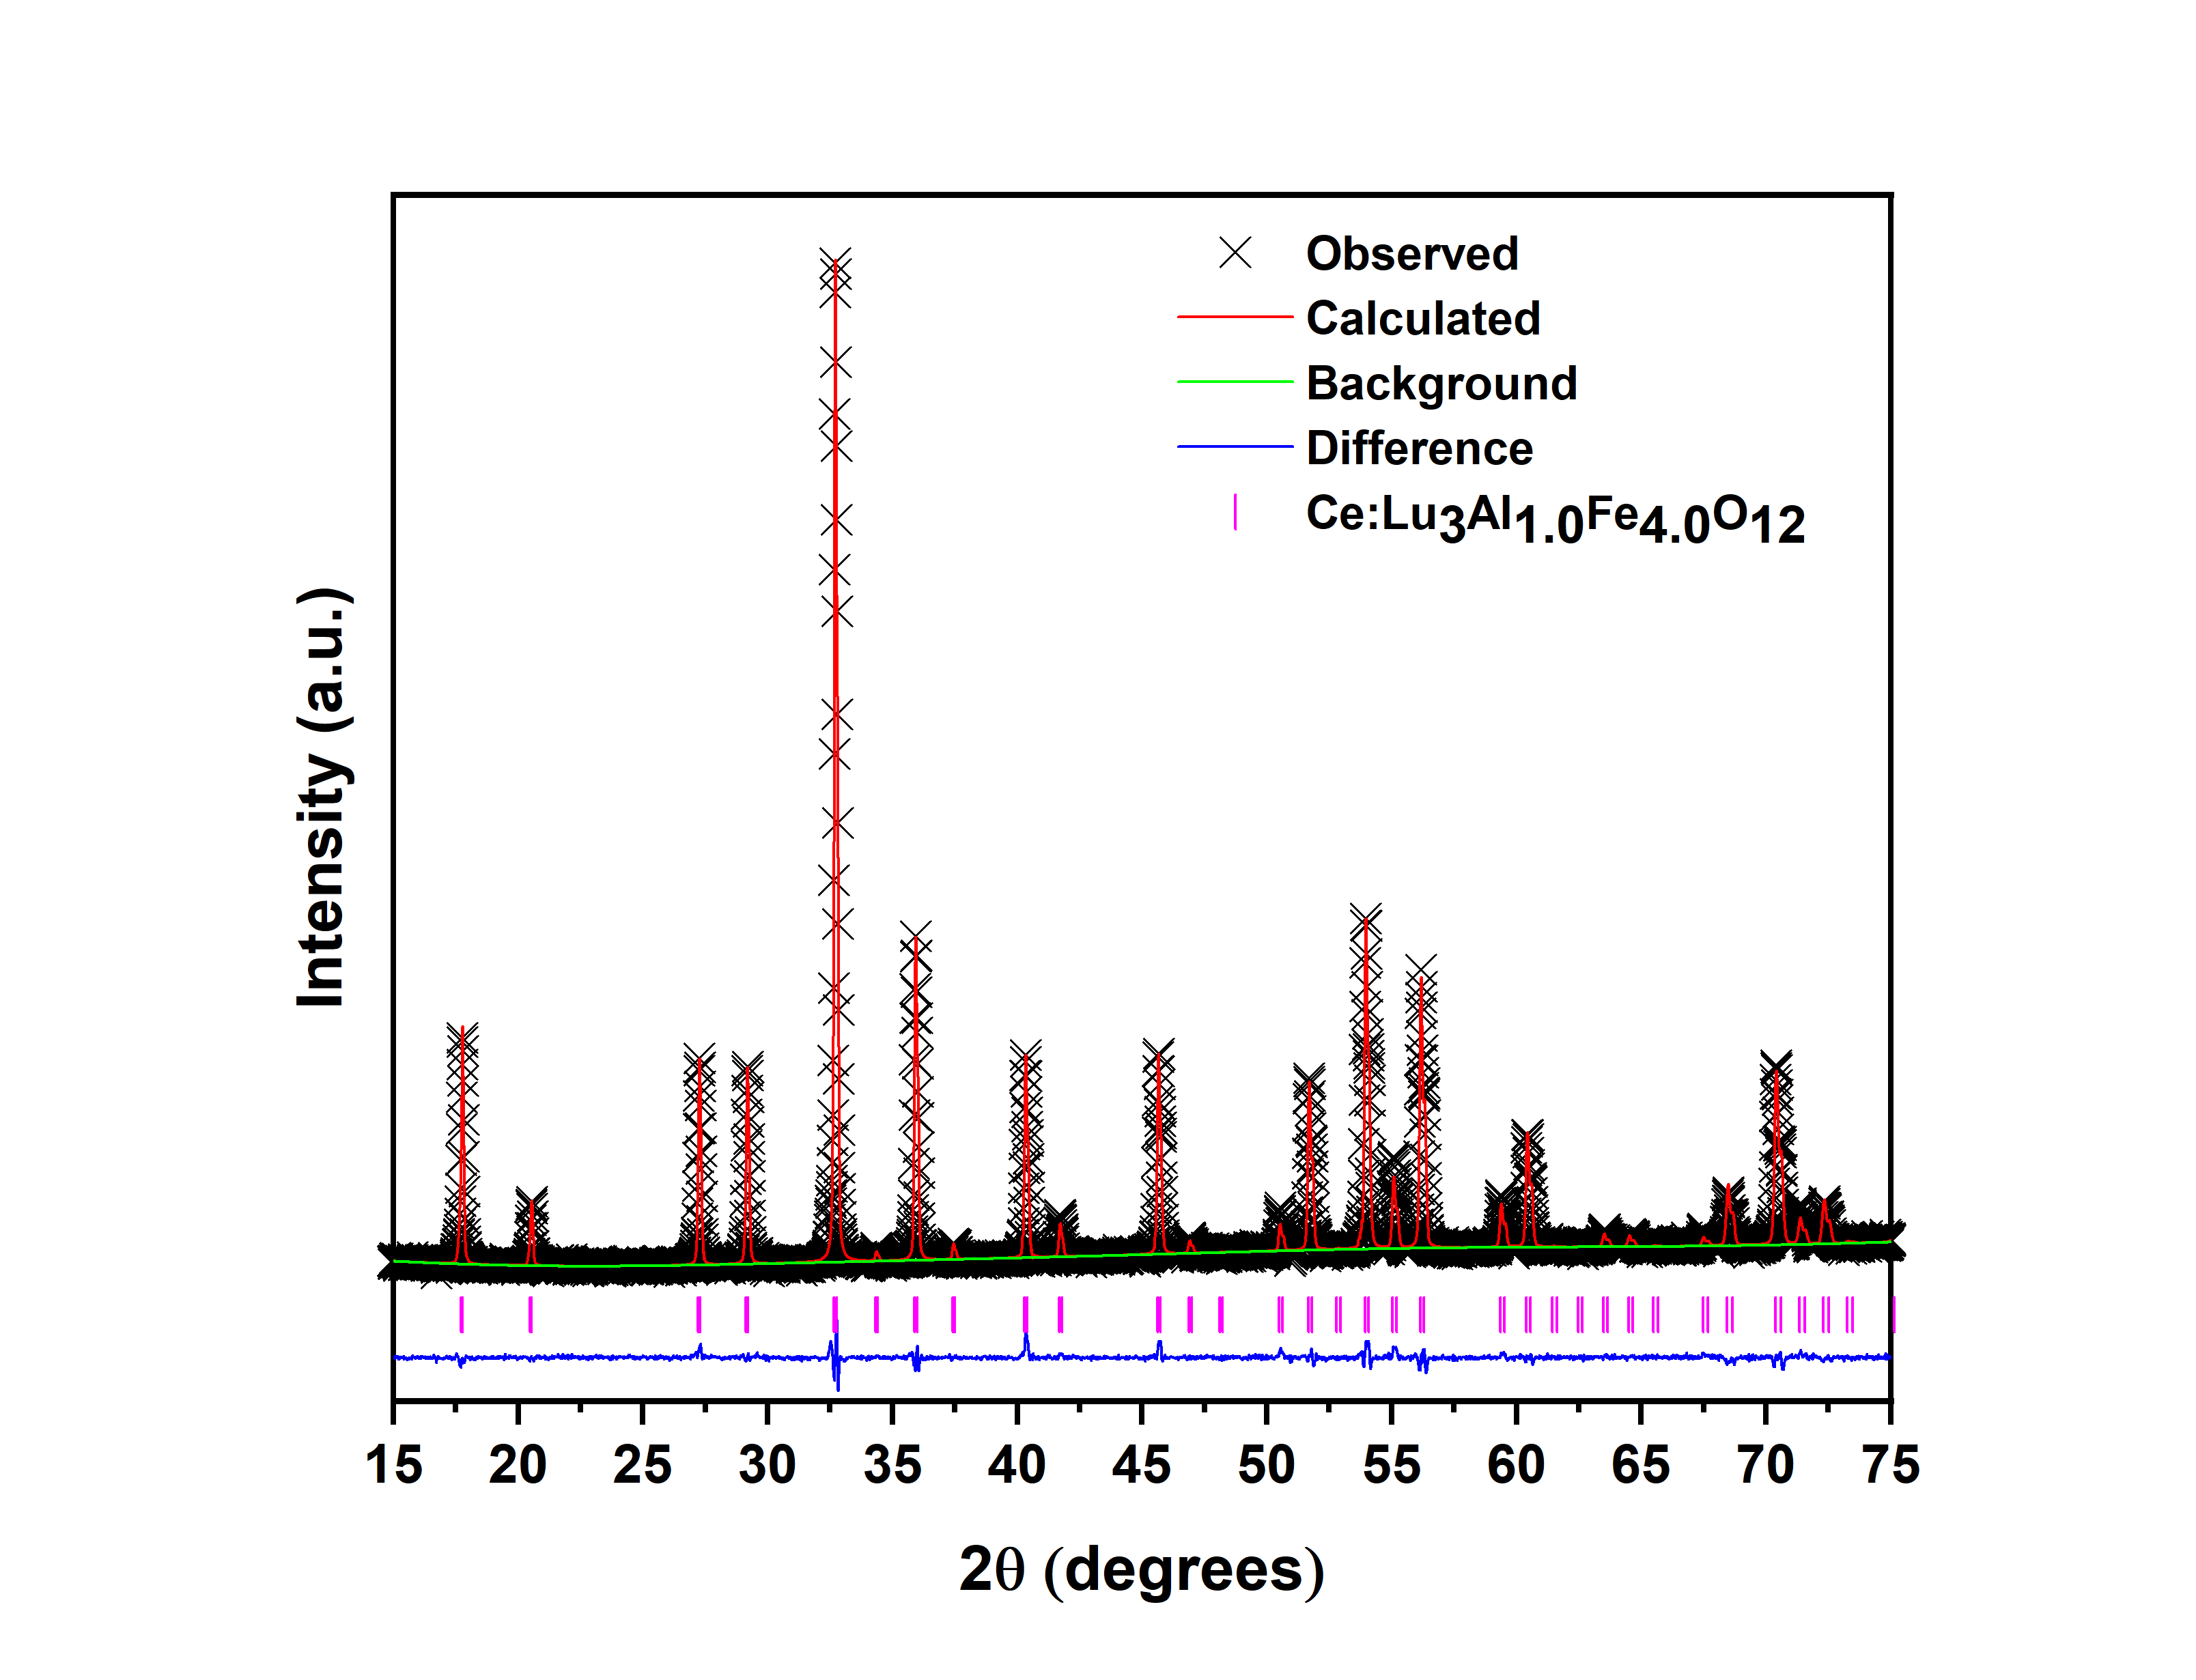
\includegraphics[width=11cm]{Anexos/x40.png}%
		\caption{Resultados de refinamiento Rietveld de
		\ce{Lu_{3.0}Al_{1.0}Fe_{4.0}O12}}\label{fig:refi40}
	\end{figure}

	\begin{figure}[t!]
		\centering%
		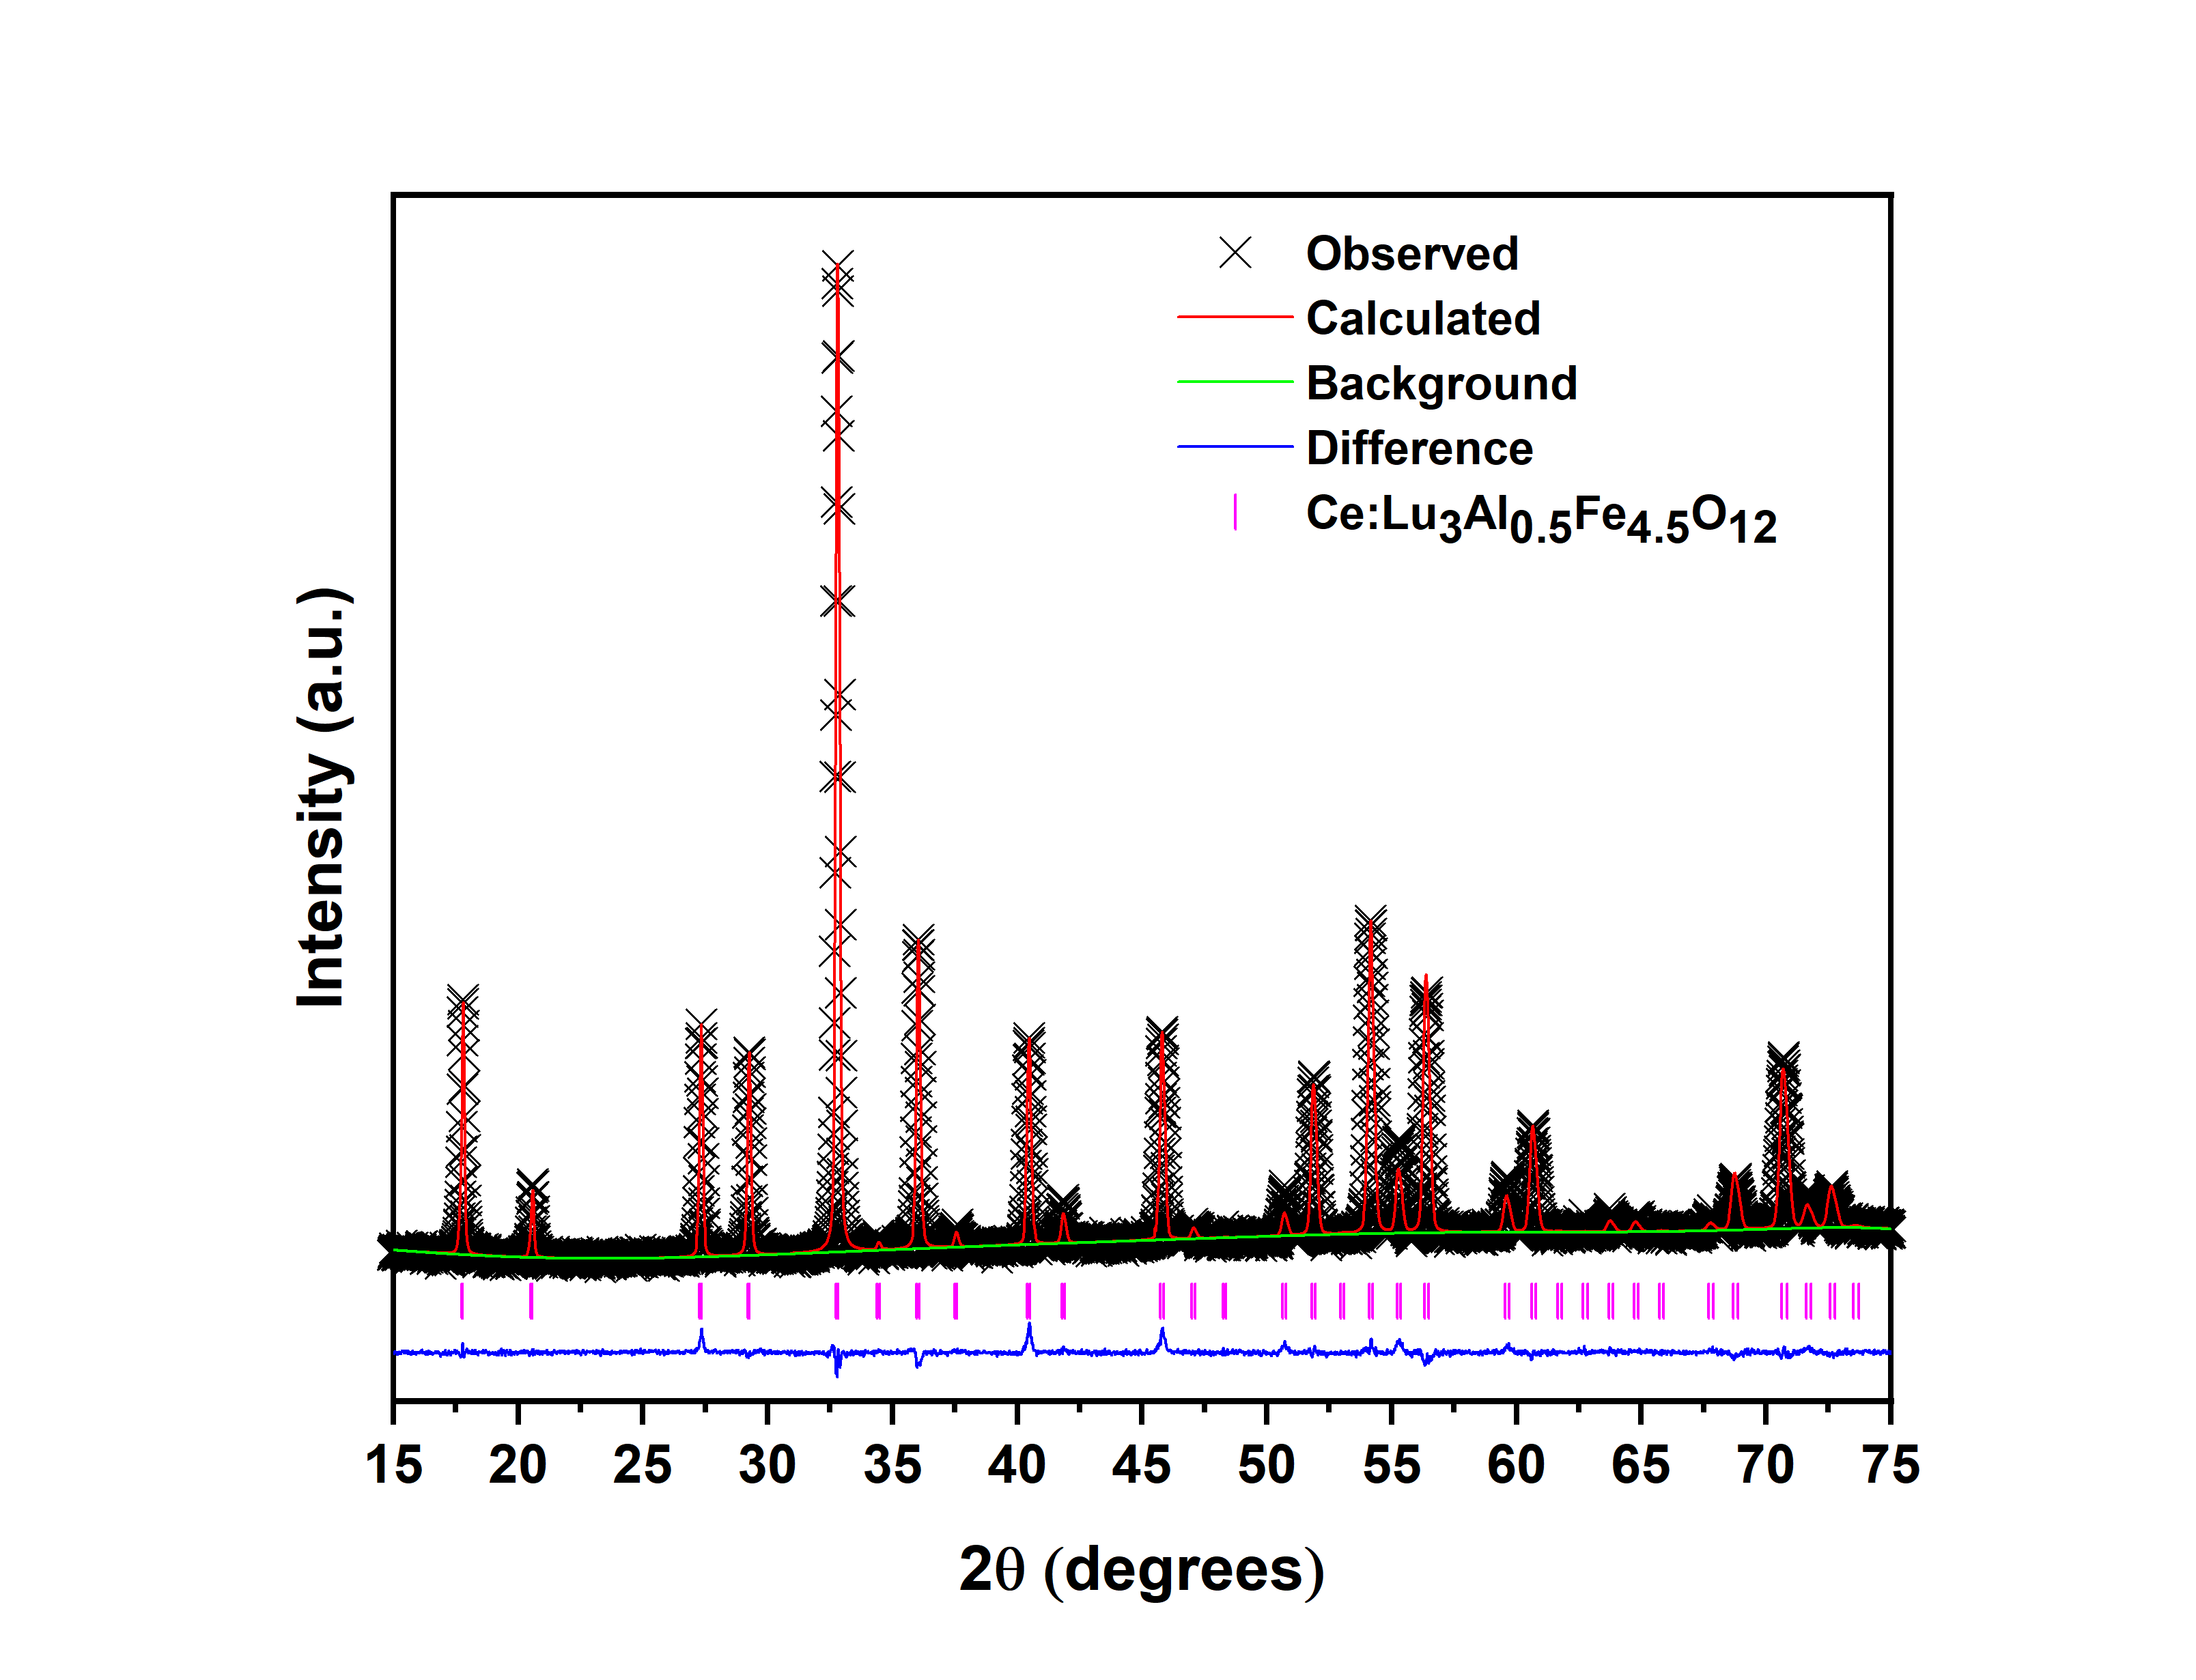
\includegraphics[width=11cm]{Anexos/x45.png}%
		\caption{Resultados de refinamiento Rietveld de
		\ce{Lu_{3.0}Al_{0.5}Fe_{4.5}O12}}\label{fig:refi45}
	\end{figure}

	\chapter{Microscopia Electrónica de Barrido}\label{AnexoC}

	\begin{figure}[h]
		\centering%

		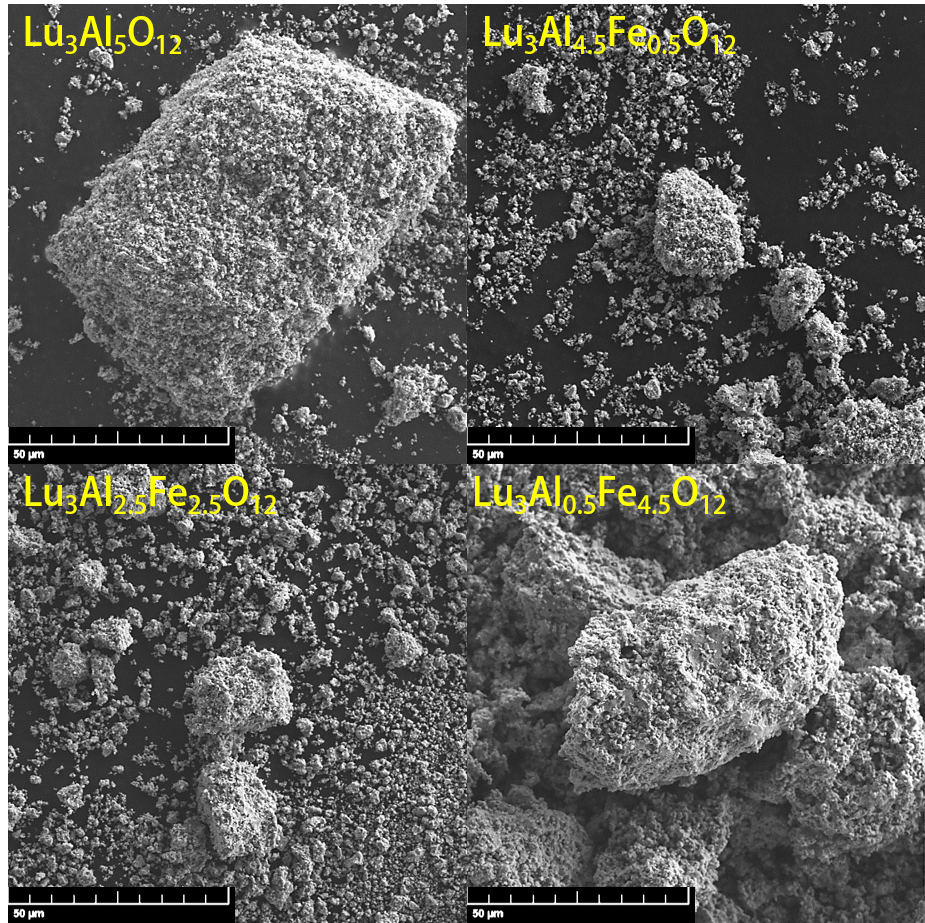
\includegraphics[width=12cm]{Kap5/sec2k.png}%
		\caption{Microscopia con electrones secundarios a 2.000 aumentos de los
		materiales \ce{Lu_{3.0}Al_{0.5}Fe_{4.5}O12} con x=0.0, 0.5, 2.5 y
		4.5}\label{fig:sec2}
	\end{figure}

	\begin{figure}[h]
		\centering%

		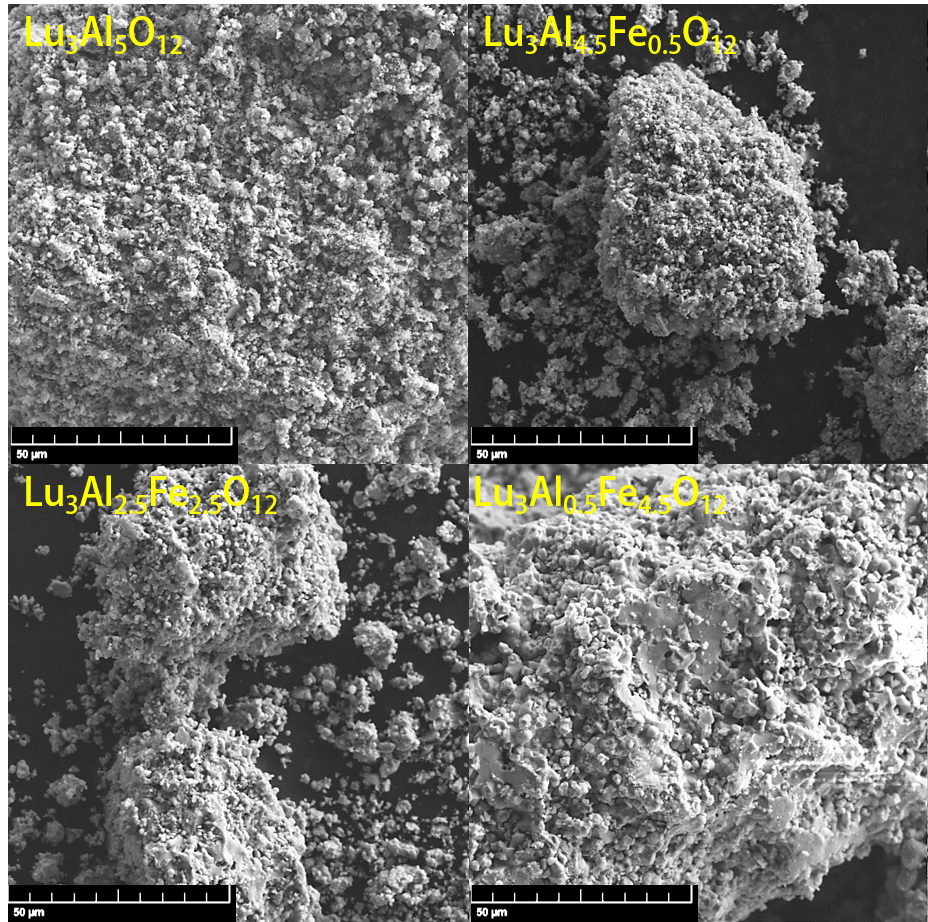
\includegraphics[width=\textwidth]{Kap5/sec5k.png}%
		\caption{Microscopia con electrones secundarios a 5.000 aumentos de los
		materiales \ce{Lu_{3.0}Al_{0.5}Fe_{4.5}O12} con x=0.0, 0.5, 2.5 y
		4.5}\label{fig:sec5}
	\end{figure}

	\begin{figure}[h]
		\centering%

		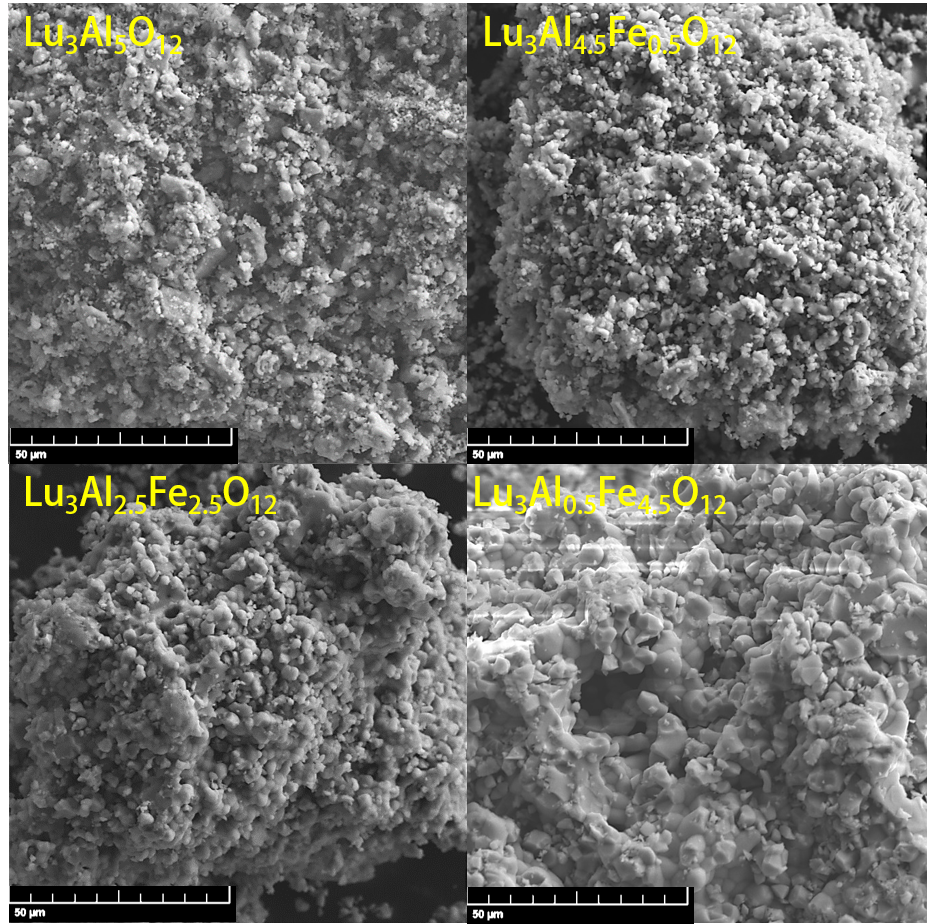
\includegraphics[width=\textwidth]{Kap5/sec10k.png}%
		\caption{Microscopia con electrones secundarios a 10.000 aumentos de los
		materiales \ce{Lu_{3.0}Al_{0.5}Fe_{4.5}O12} con x=0.0, 0.5, 2.5 y
		4.5}\label{fig:sec10}
	\end{figure}

	\begin{figure}[h]
		\centering%

		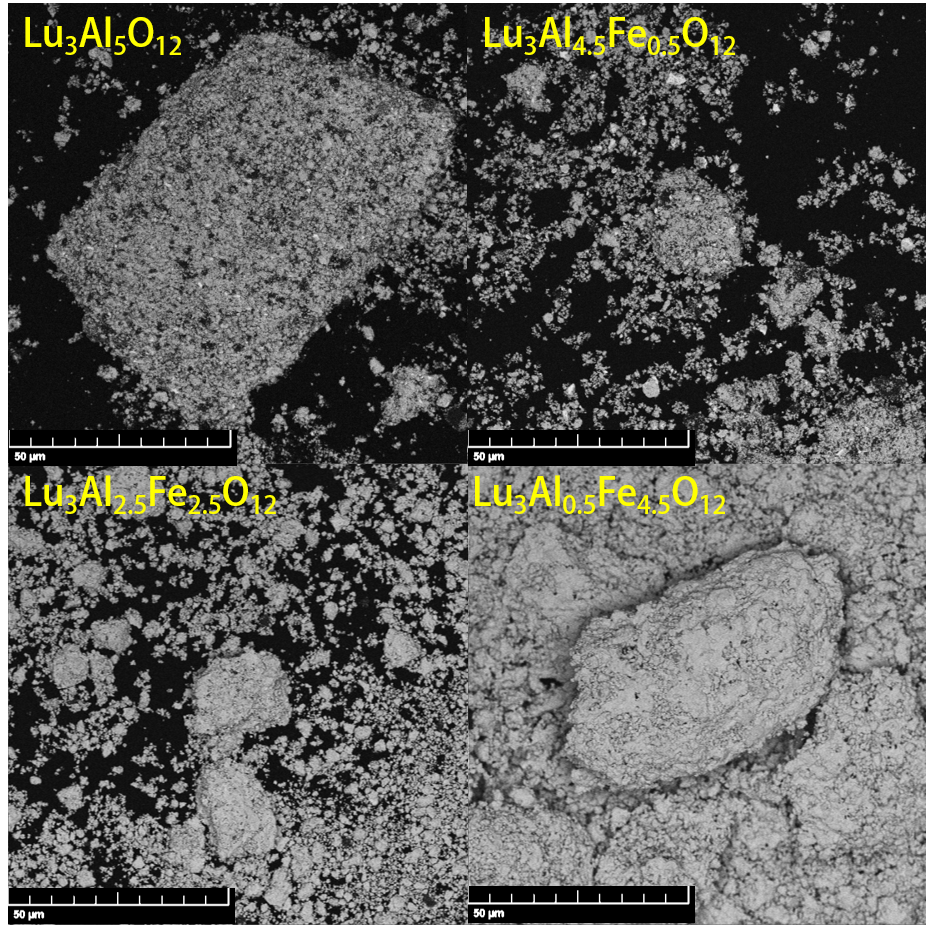
\includegraphics[width=\textwidth]{Kap5/ret2k.png}%
		\caption{Microscopia con electrones retrodispersados a 2.000 aumentos de los
		materiales \ce{Lu_{3.0}Al_{0.5}Fe_{4.5}O12} con x=0.0, 0.5, 2.5 y
		4.5}\label{fig:ret2}
	\end{figure}

	\begin{figure}[h]
		\centering%

		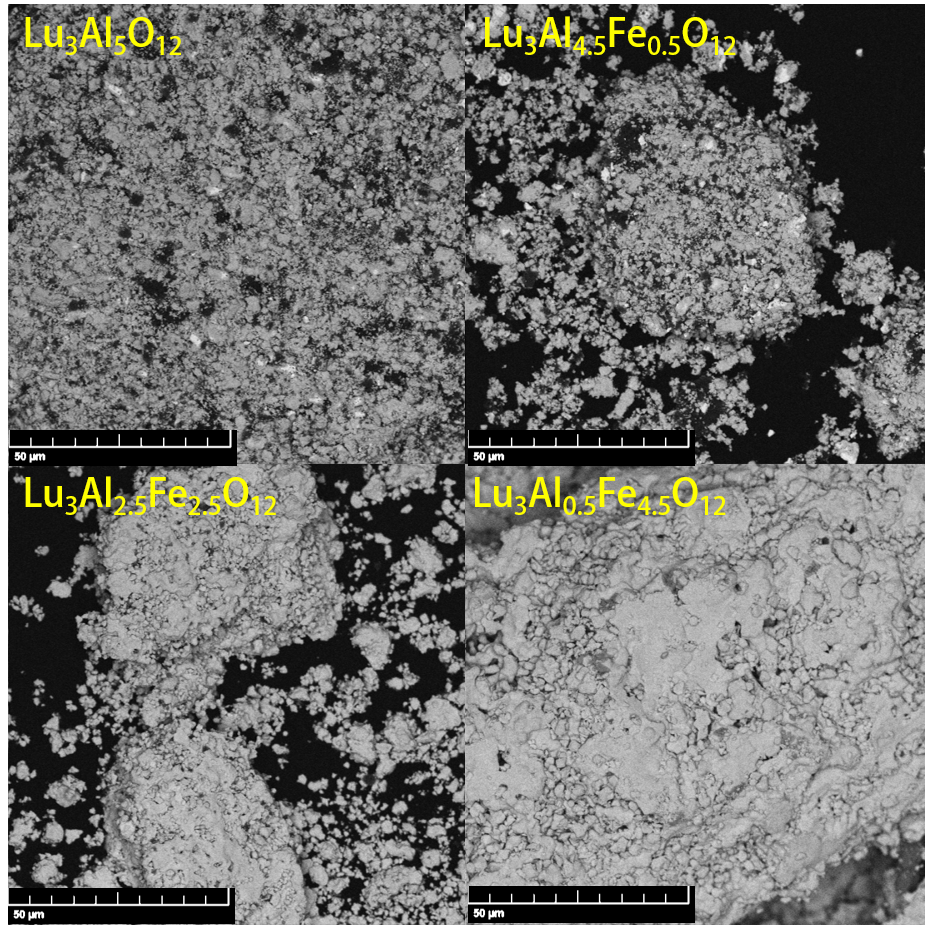
\includegraphics[width=\textwidth]{Kap5/ret5k.png}%
		\caption{Microscopia con electrones retrodispersados a 5.000 aumentos de los
		materiales \ce{Lu_{3.0}Al_{0.5}Fe_{4.5}O12} con x=0.0, 0.5, 2.5 y
		4.5}\label{fig:ret5}
	\end{figure}

	\begin{figure}[h]
		\centering%

		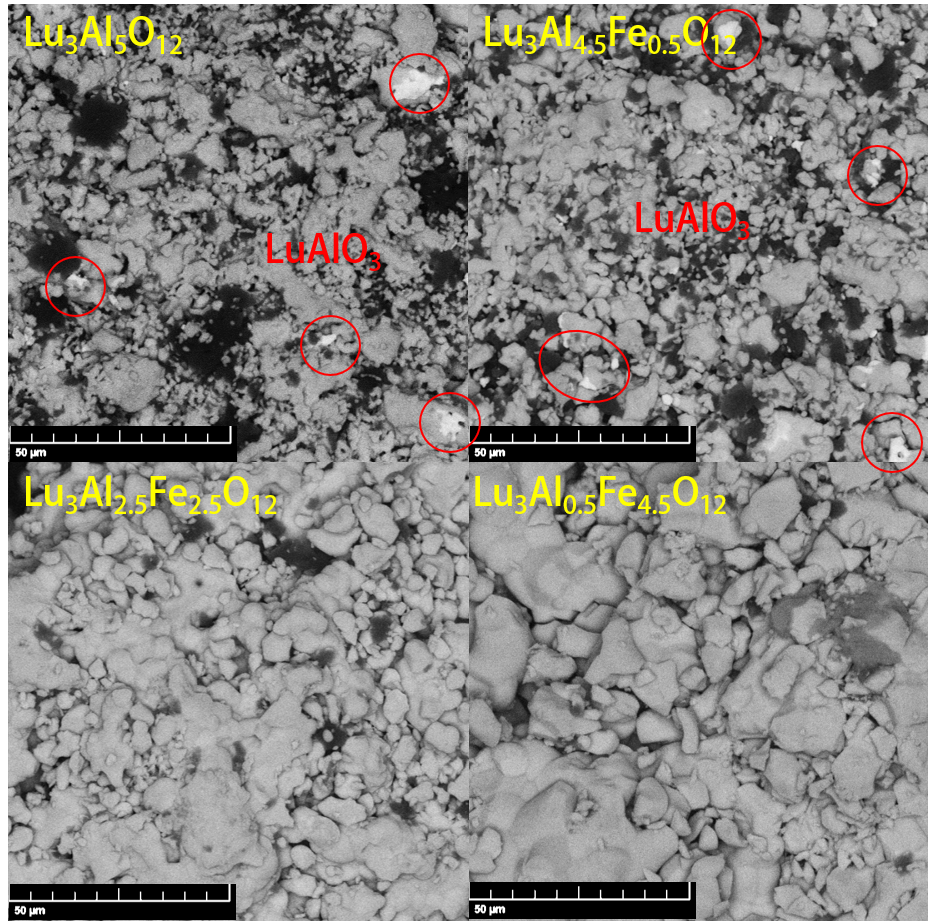
\includegraphics[width=\textwidth]{Kap5/ret20k.png}%
		\caption{Microscopia con electrones retrodispersados a 20.000 aumentos de los
		materiales \ce{Lu_{3.0}Al_{0.5}Fe_{4.5}O12} con x=0.0, 0.5, 2.5 y
		4.5}\label{fig:ret20}
	\end{figure}

	\begin{figure}[h]
		\centering%

		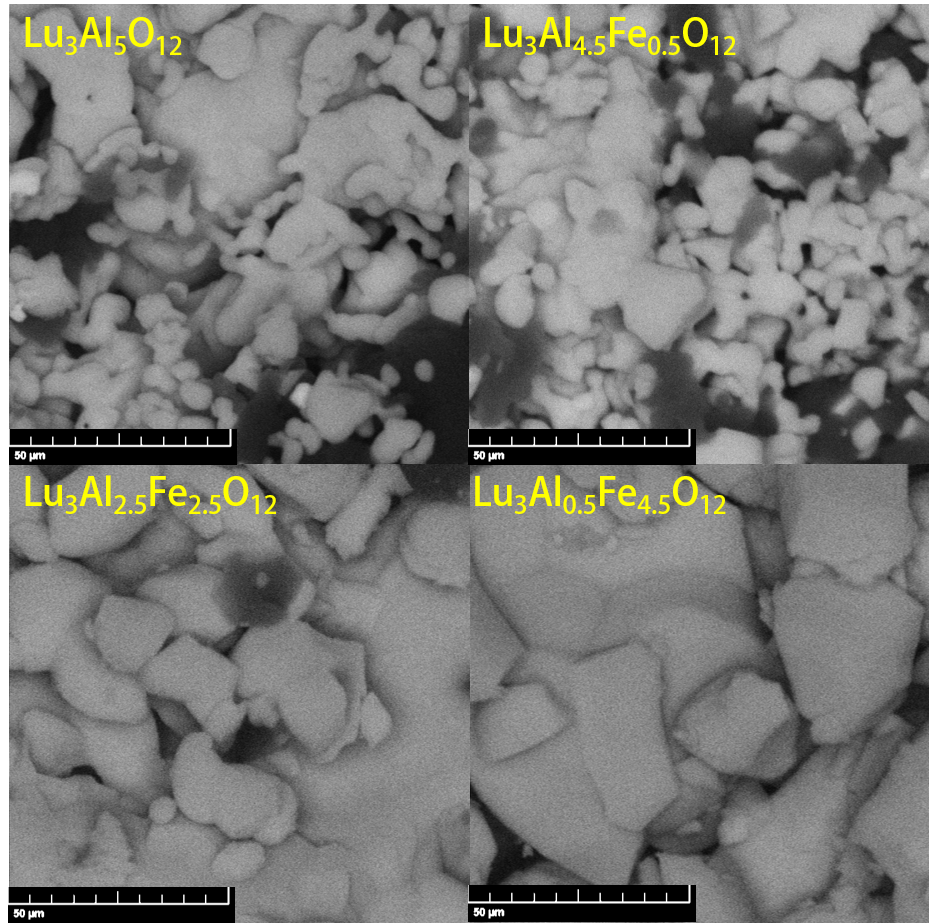
\includegraphics[width=\textwidth]{Kap5/ret90k.png}%
		\caption{Microscopia con electrones retrodispersados a 2.000 aumentos de los
		materiales \ce{Lu_{3.0}Al_{0.5}Fe_{4.5}O12} con x=0.0, 0.5, 2.5 y
		4.5}\label{fig:ret90}
	\end{figure}

	\chapter{Tamaño de Partícula}\label{AnexoD}

	\begin{figure}[h]
		\centering%

		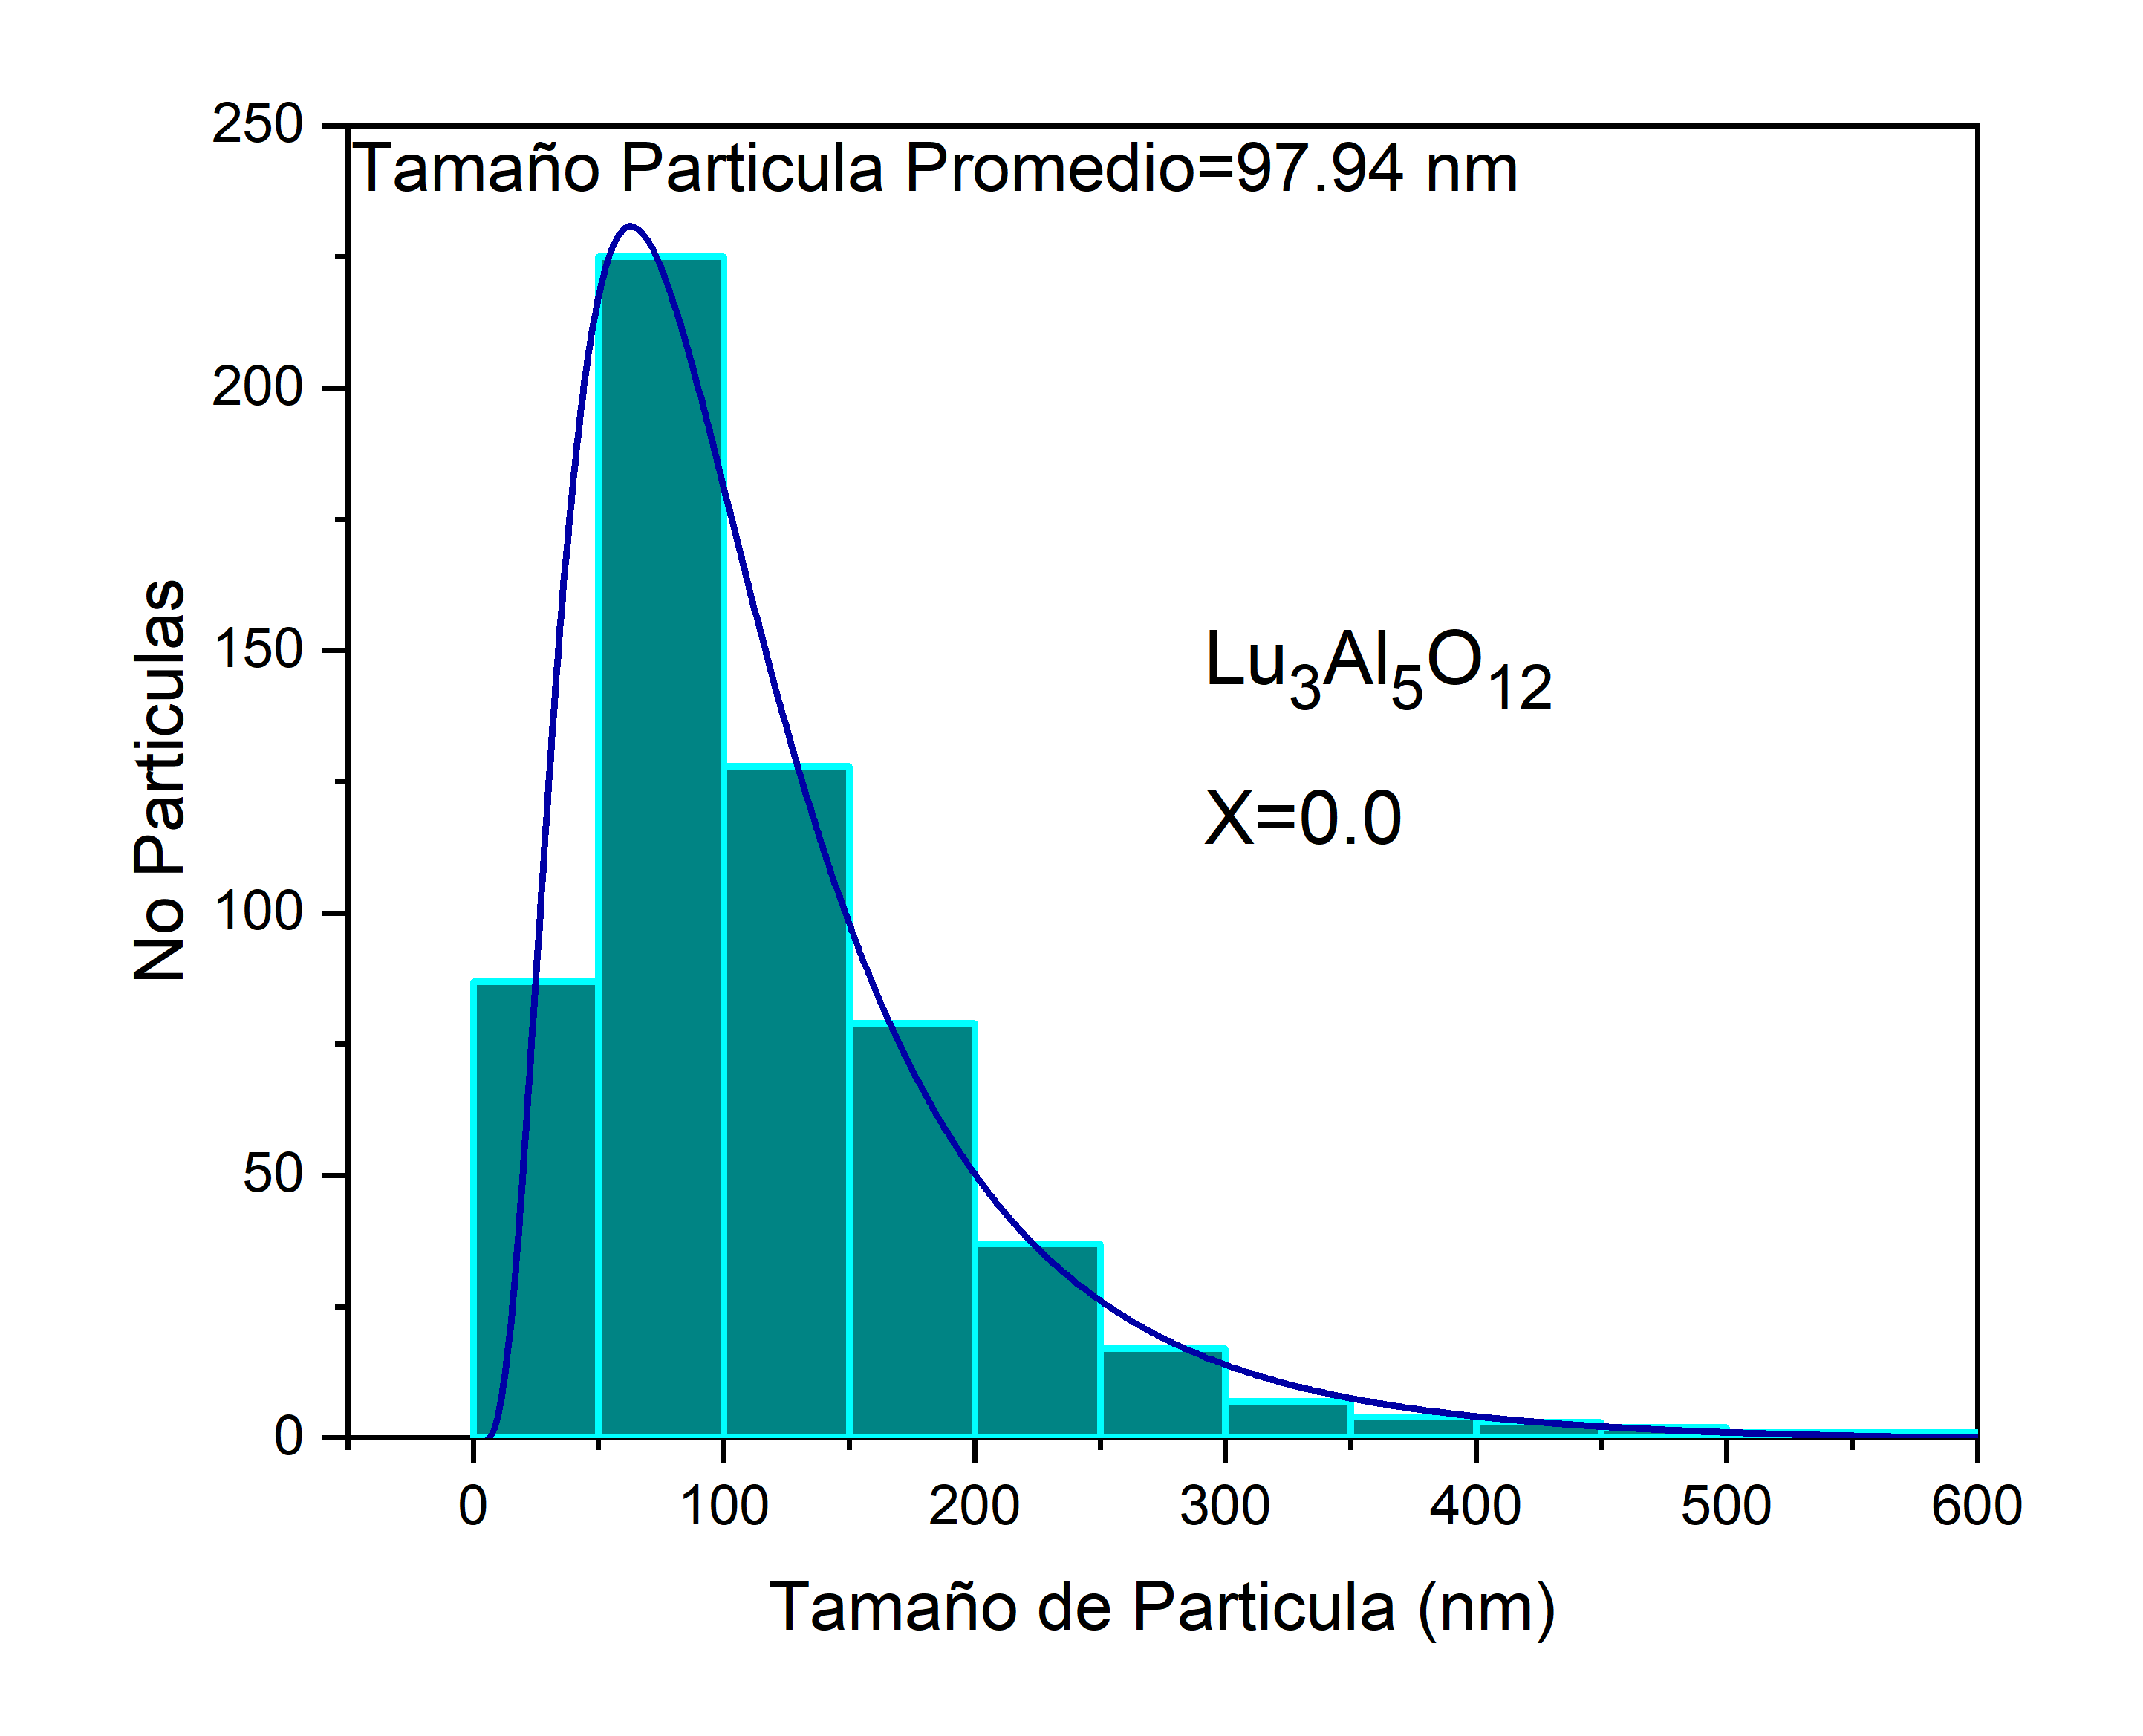
\includegraphics[width=13cm]{Kap5/TamG0.png}%
		\caption{Distribución del tamaño de partícula para \ce{Lu_{3.0}Al_{5.0}O12} medida mediante ImageJ}\label{fig:tamG0}
	\end{figure}

	\begin{figure}[h]
		\centering%

		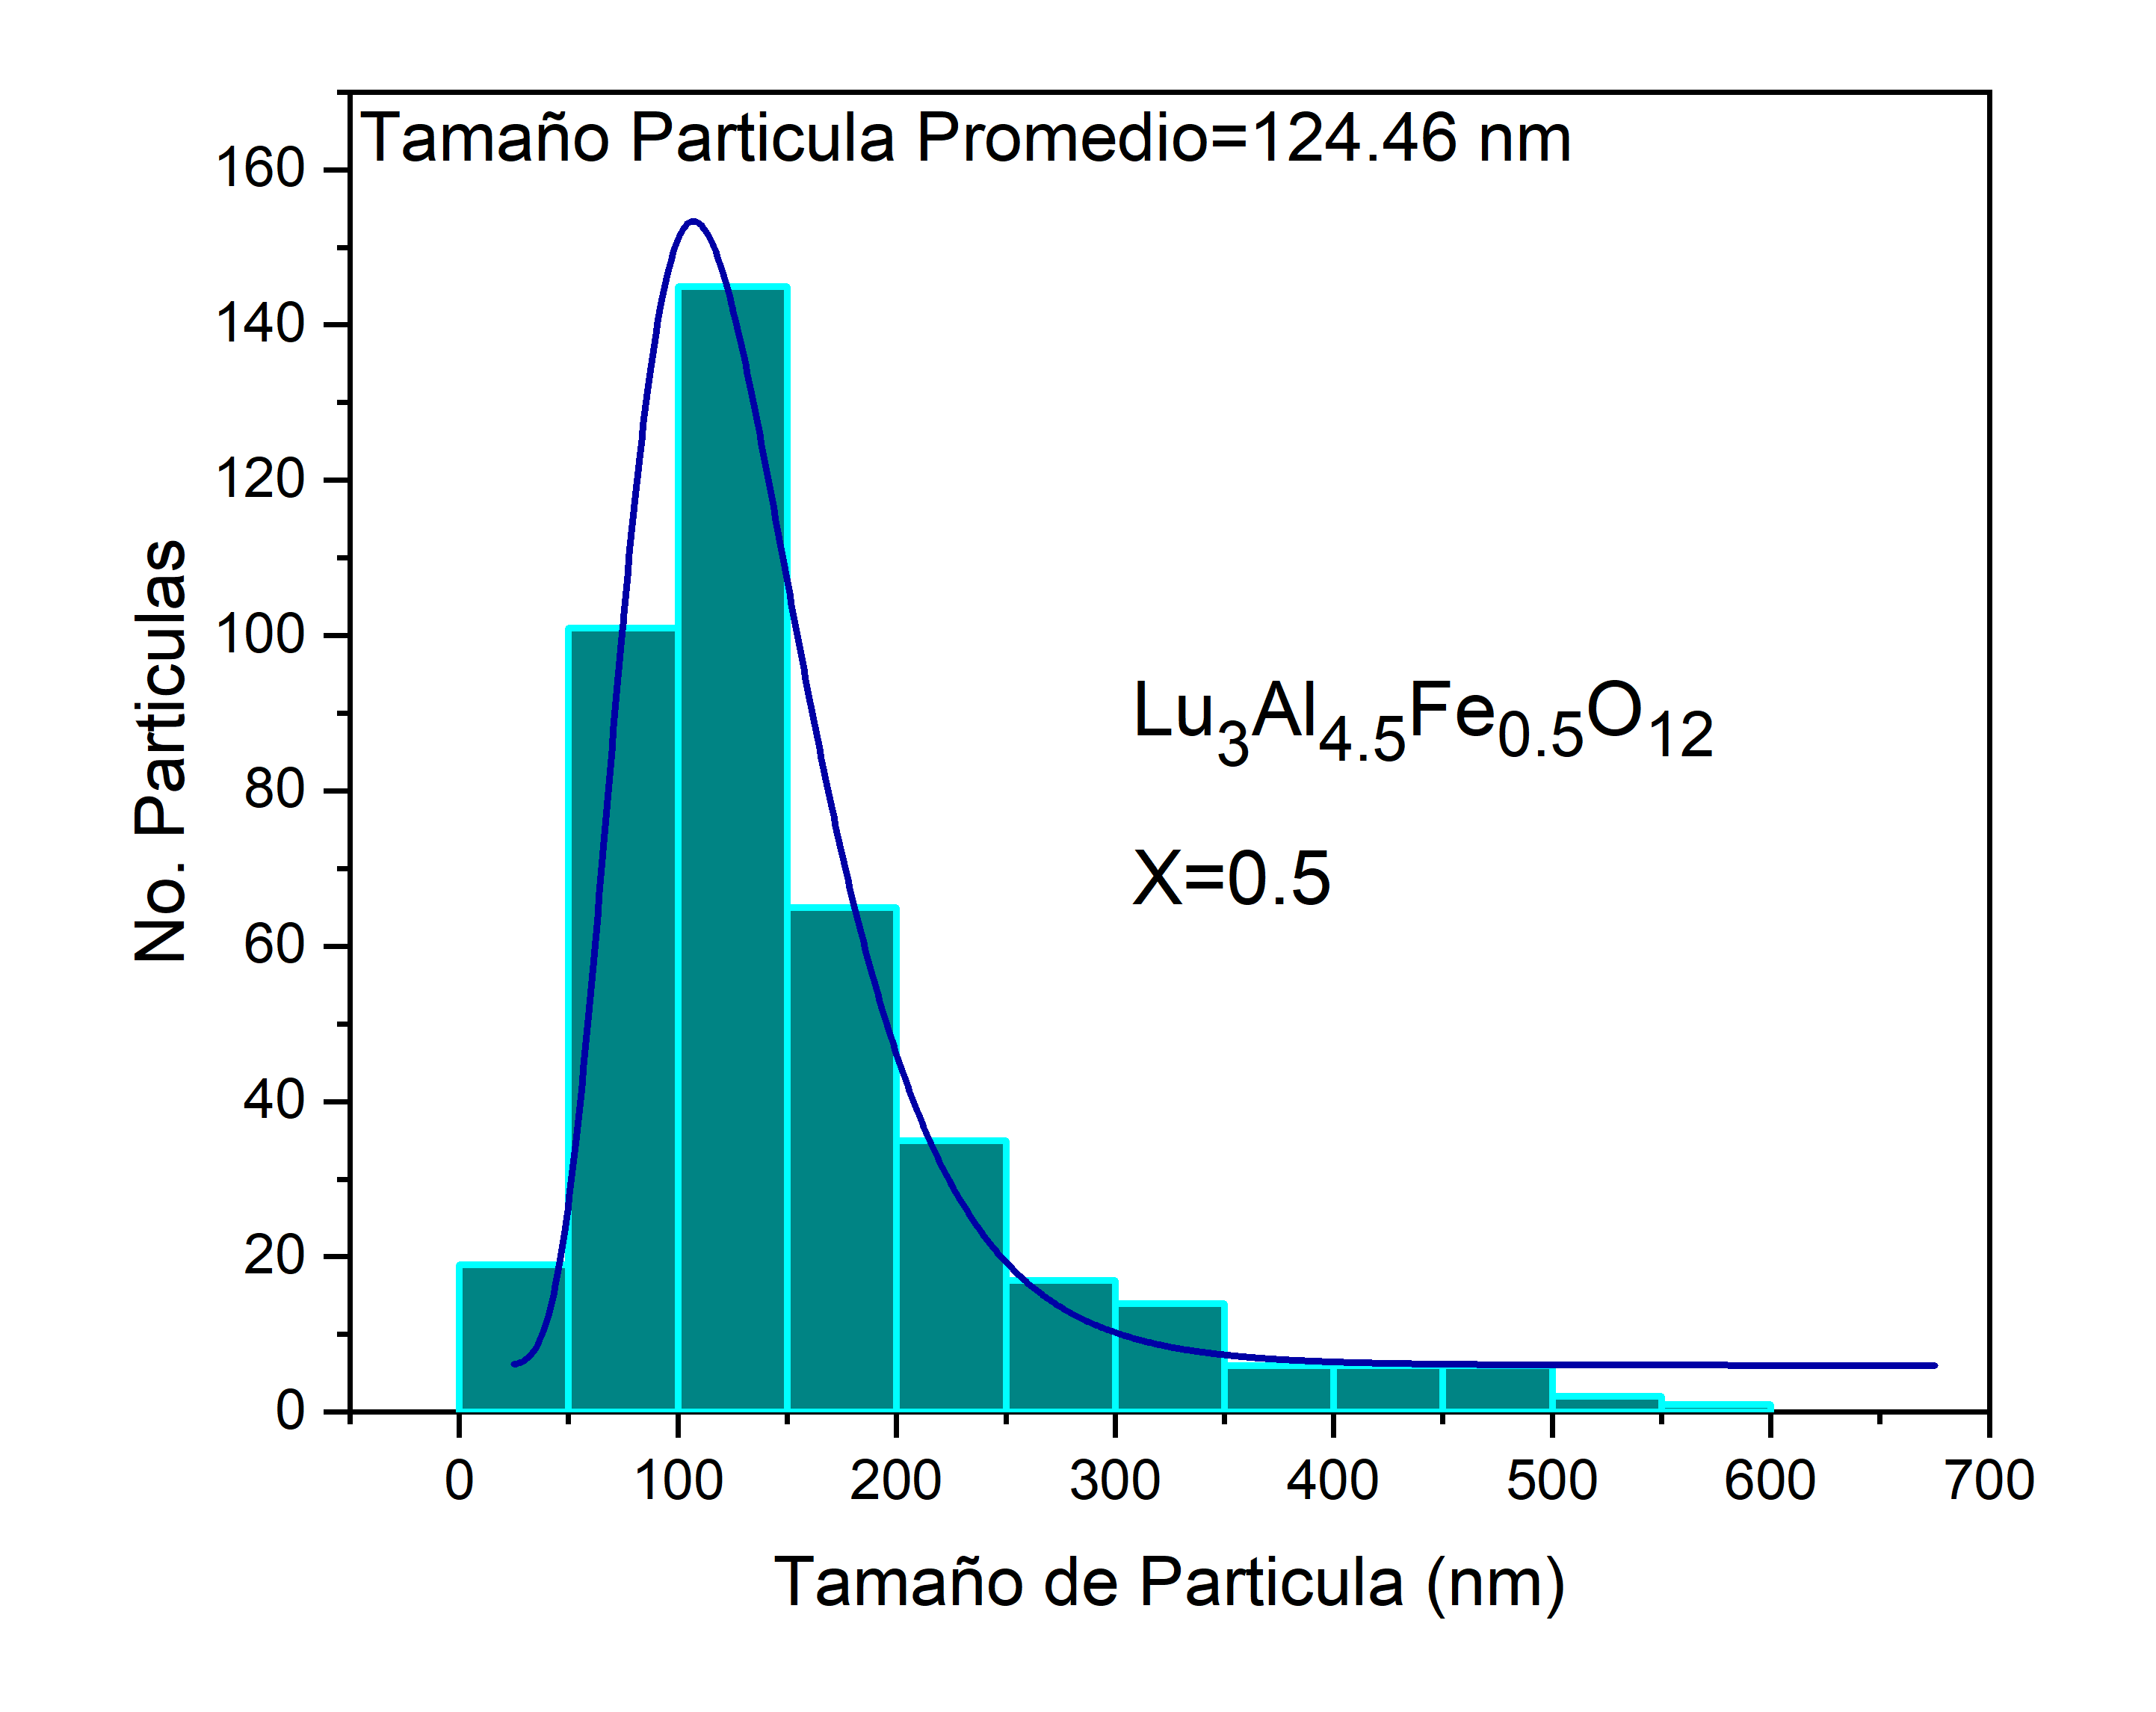
\includegraphics[width=\textwidth]{Kap5/TamG1.png}%
		\caption{Distribución del tamaño de partícula para \ce{Lu_{3.0}Al_{4.5}Fe_{0.5}O12} medida mediante ImageJ}\label{fig:tamG1}
	\end{figure}

	\begin{figure}[h]
		\centering%

		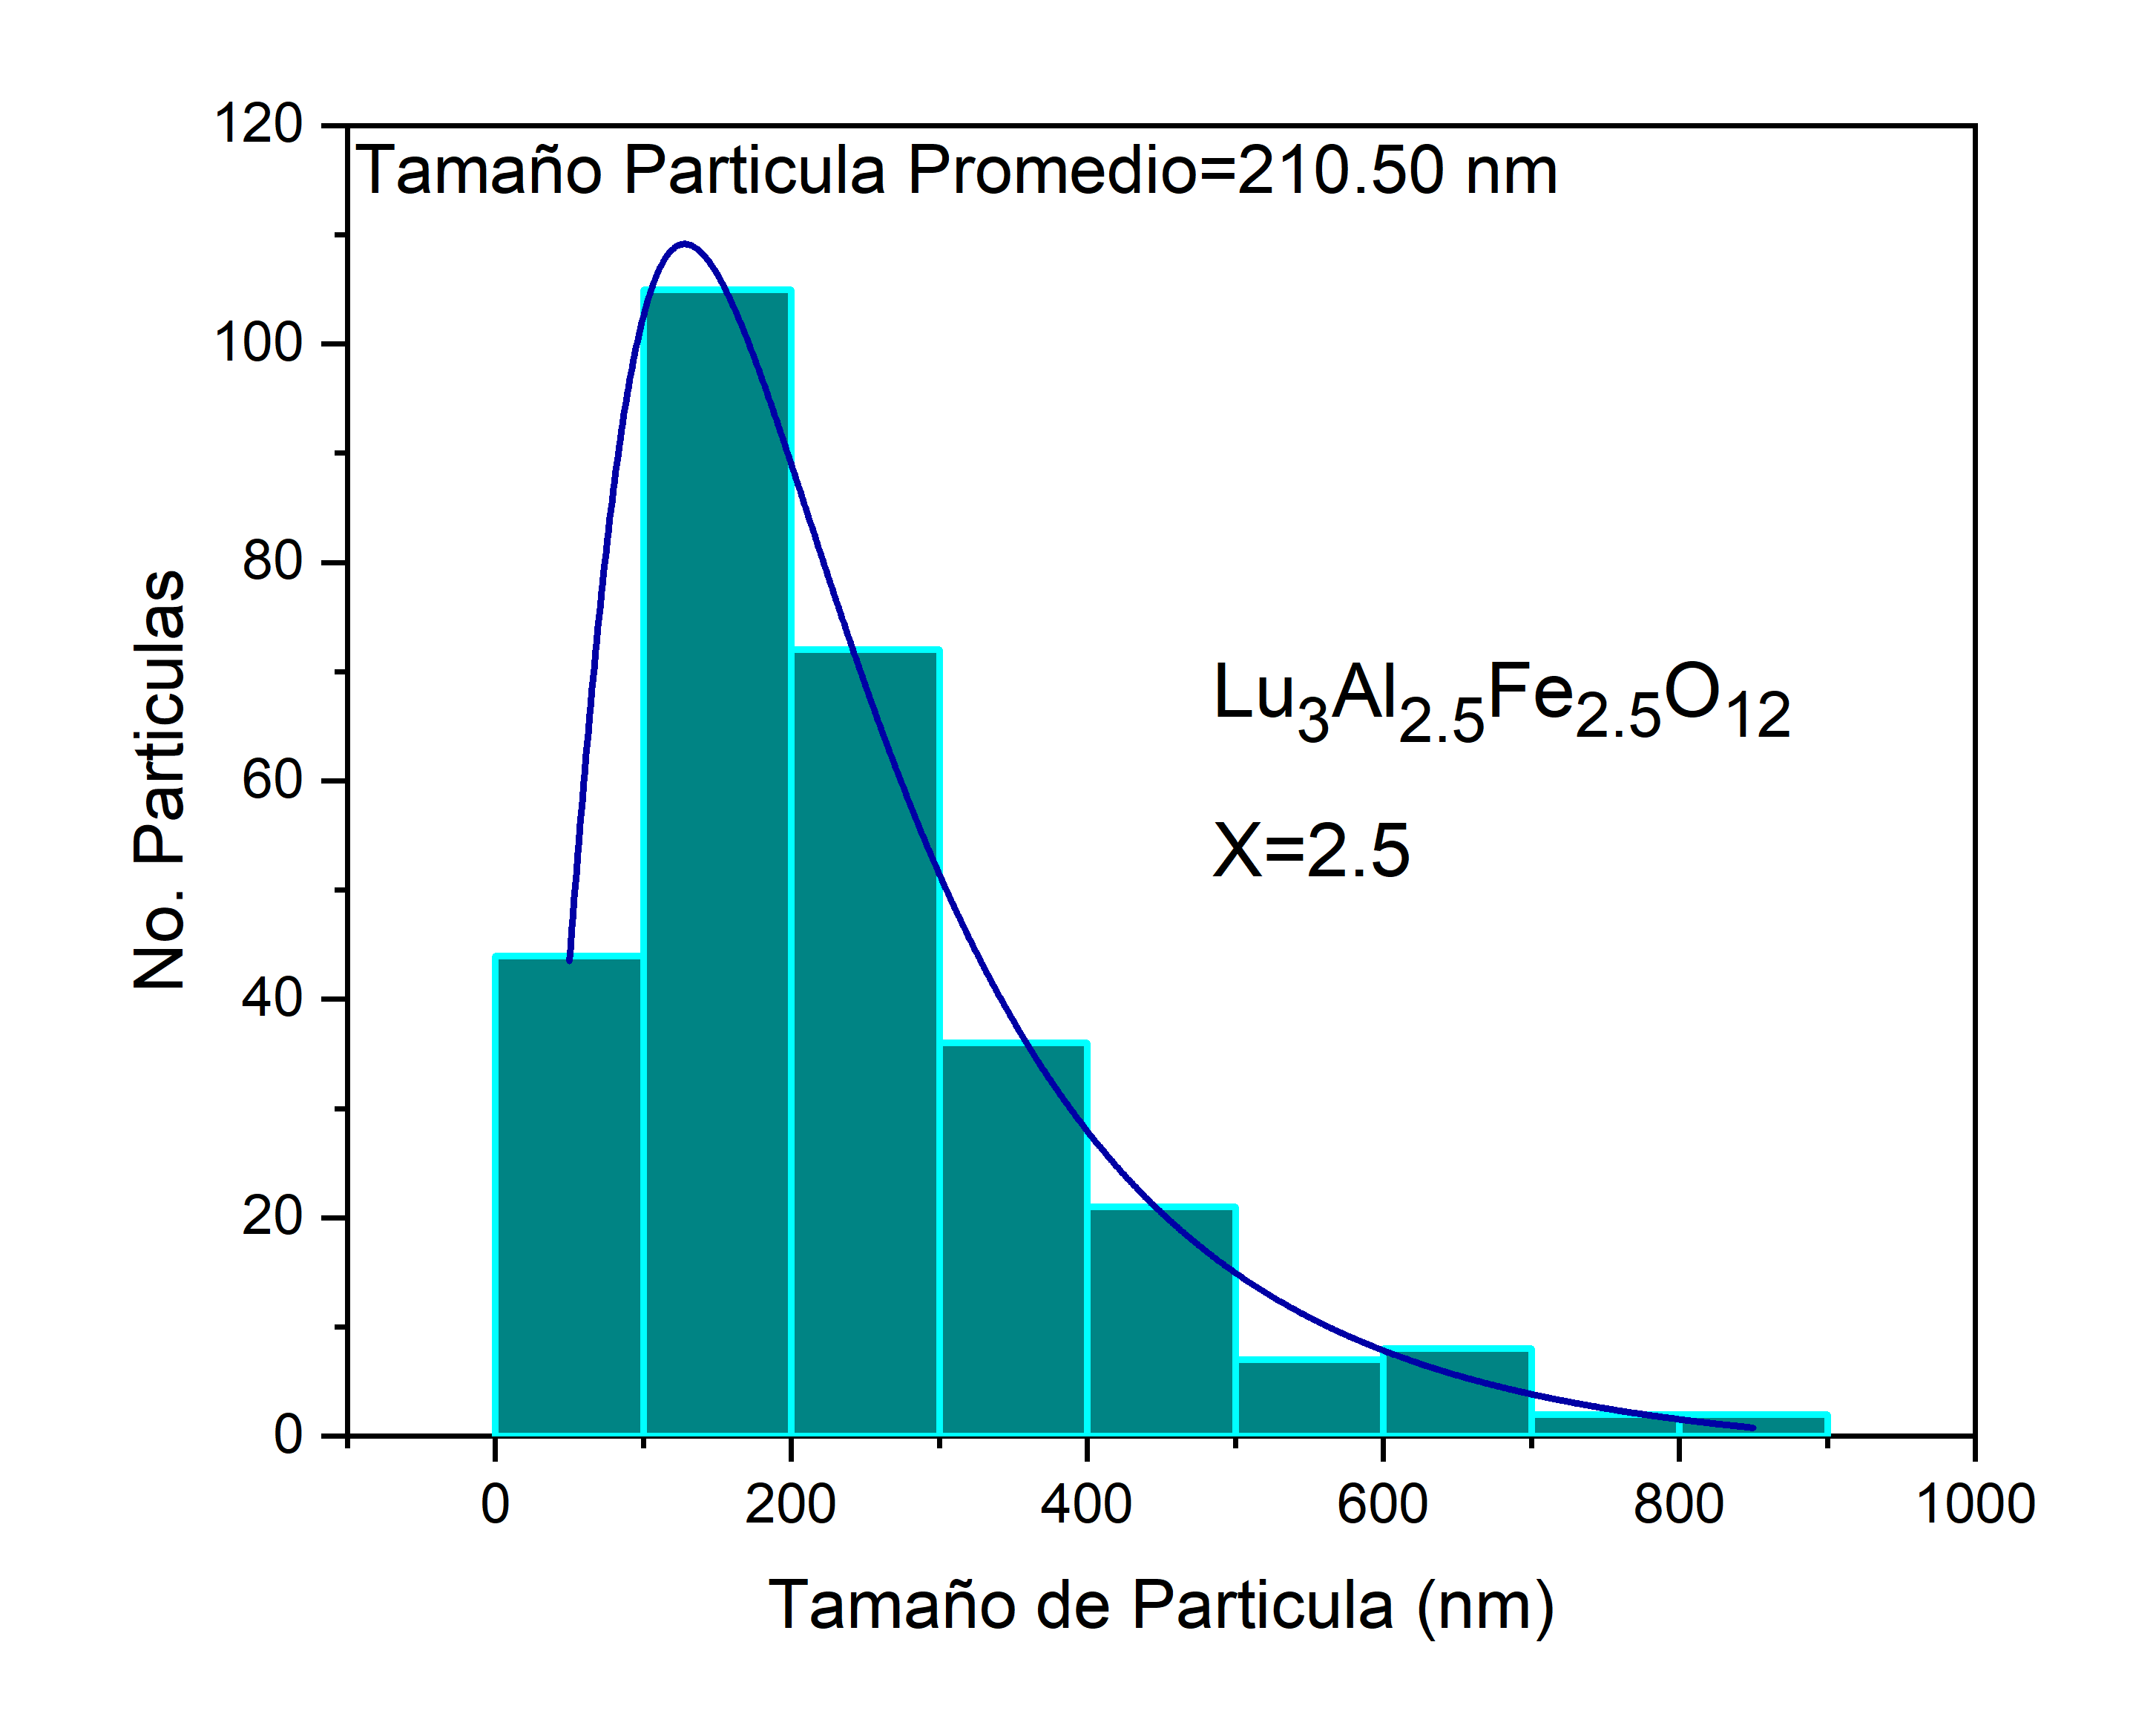
\includegraphics[width=\textwidth]{Kap5/TamG5.png}%
		\caption{Distribución del tamaño de partícula para \ce{Lu_{3.0}Al_{2.5}Fe_{2.5}O12} medida mediante ImageJ}\label{fig:tamG5}
	\end{figure}

	\begin{figure}[h]
		\centering%

		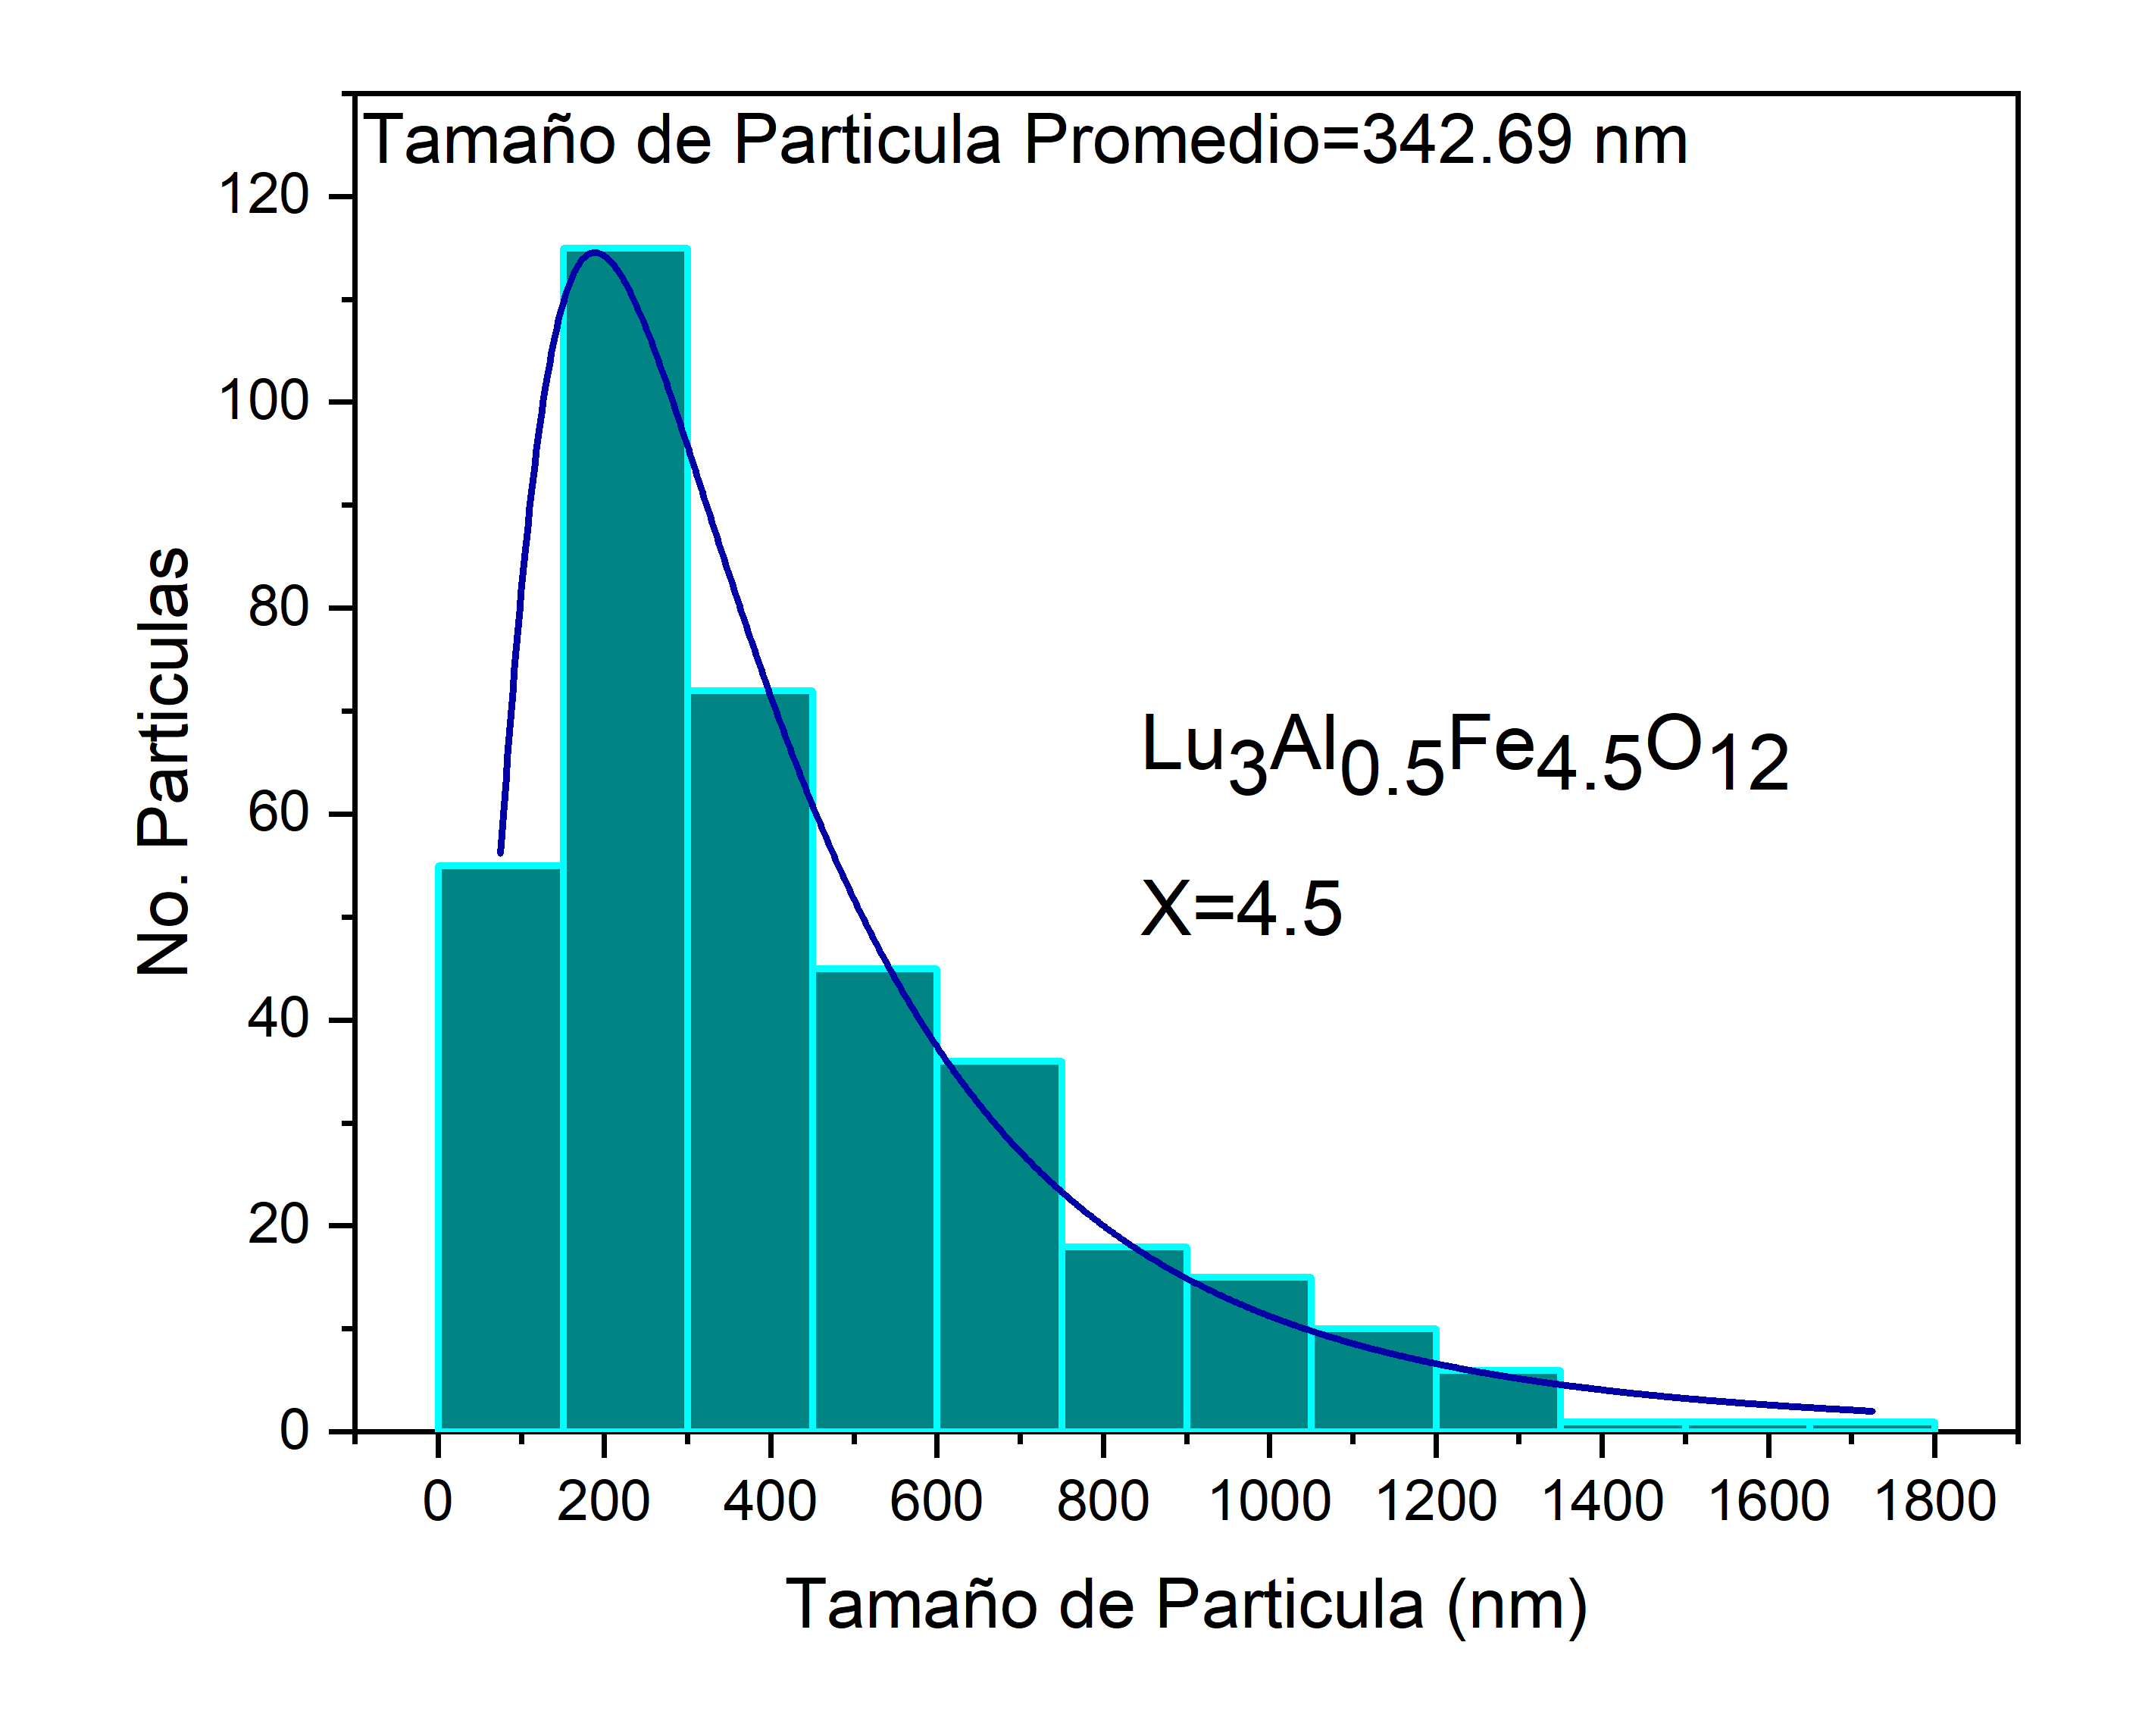
\includegraphics[width=\textwidth]{Kap5/TamG9.png}%
		\caption{Distribución del tamaño de partícula para \ce{Lu_{3.0}Al_{0.5}Fe_{4.5}O12} medida mediante ImageJ}\label{fig:tamG9}
	\end{figure}

	\chapter{EDX}\label{edx}

	\begin{figure}[h]
		\centering%

		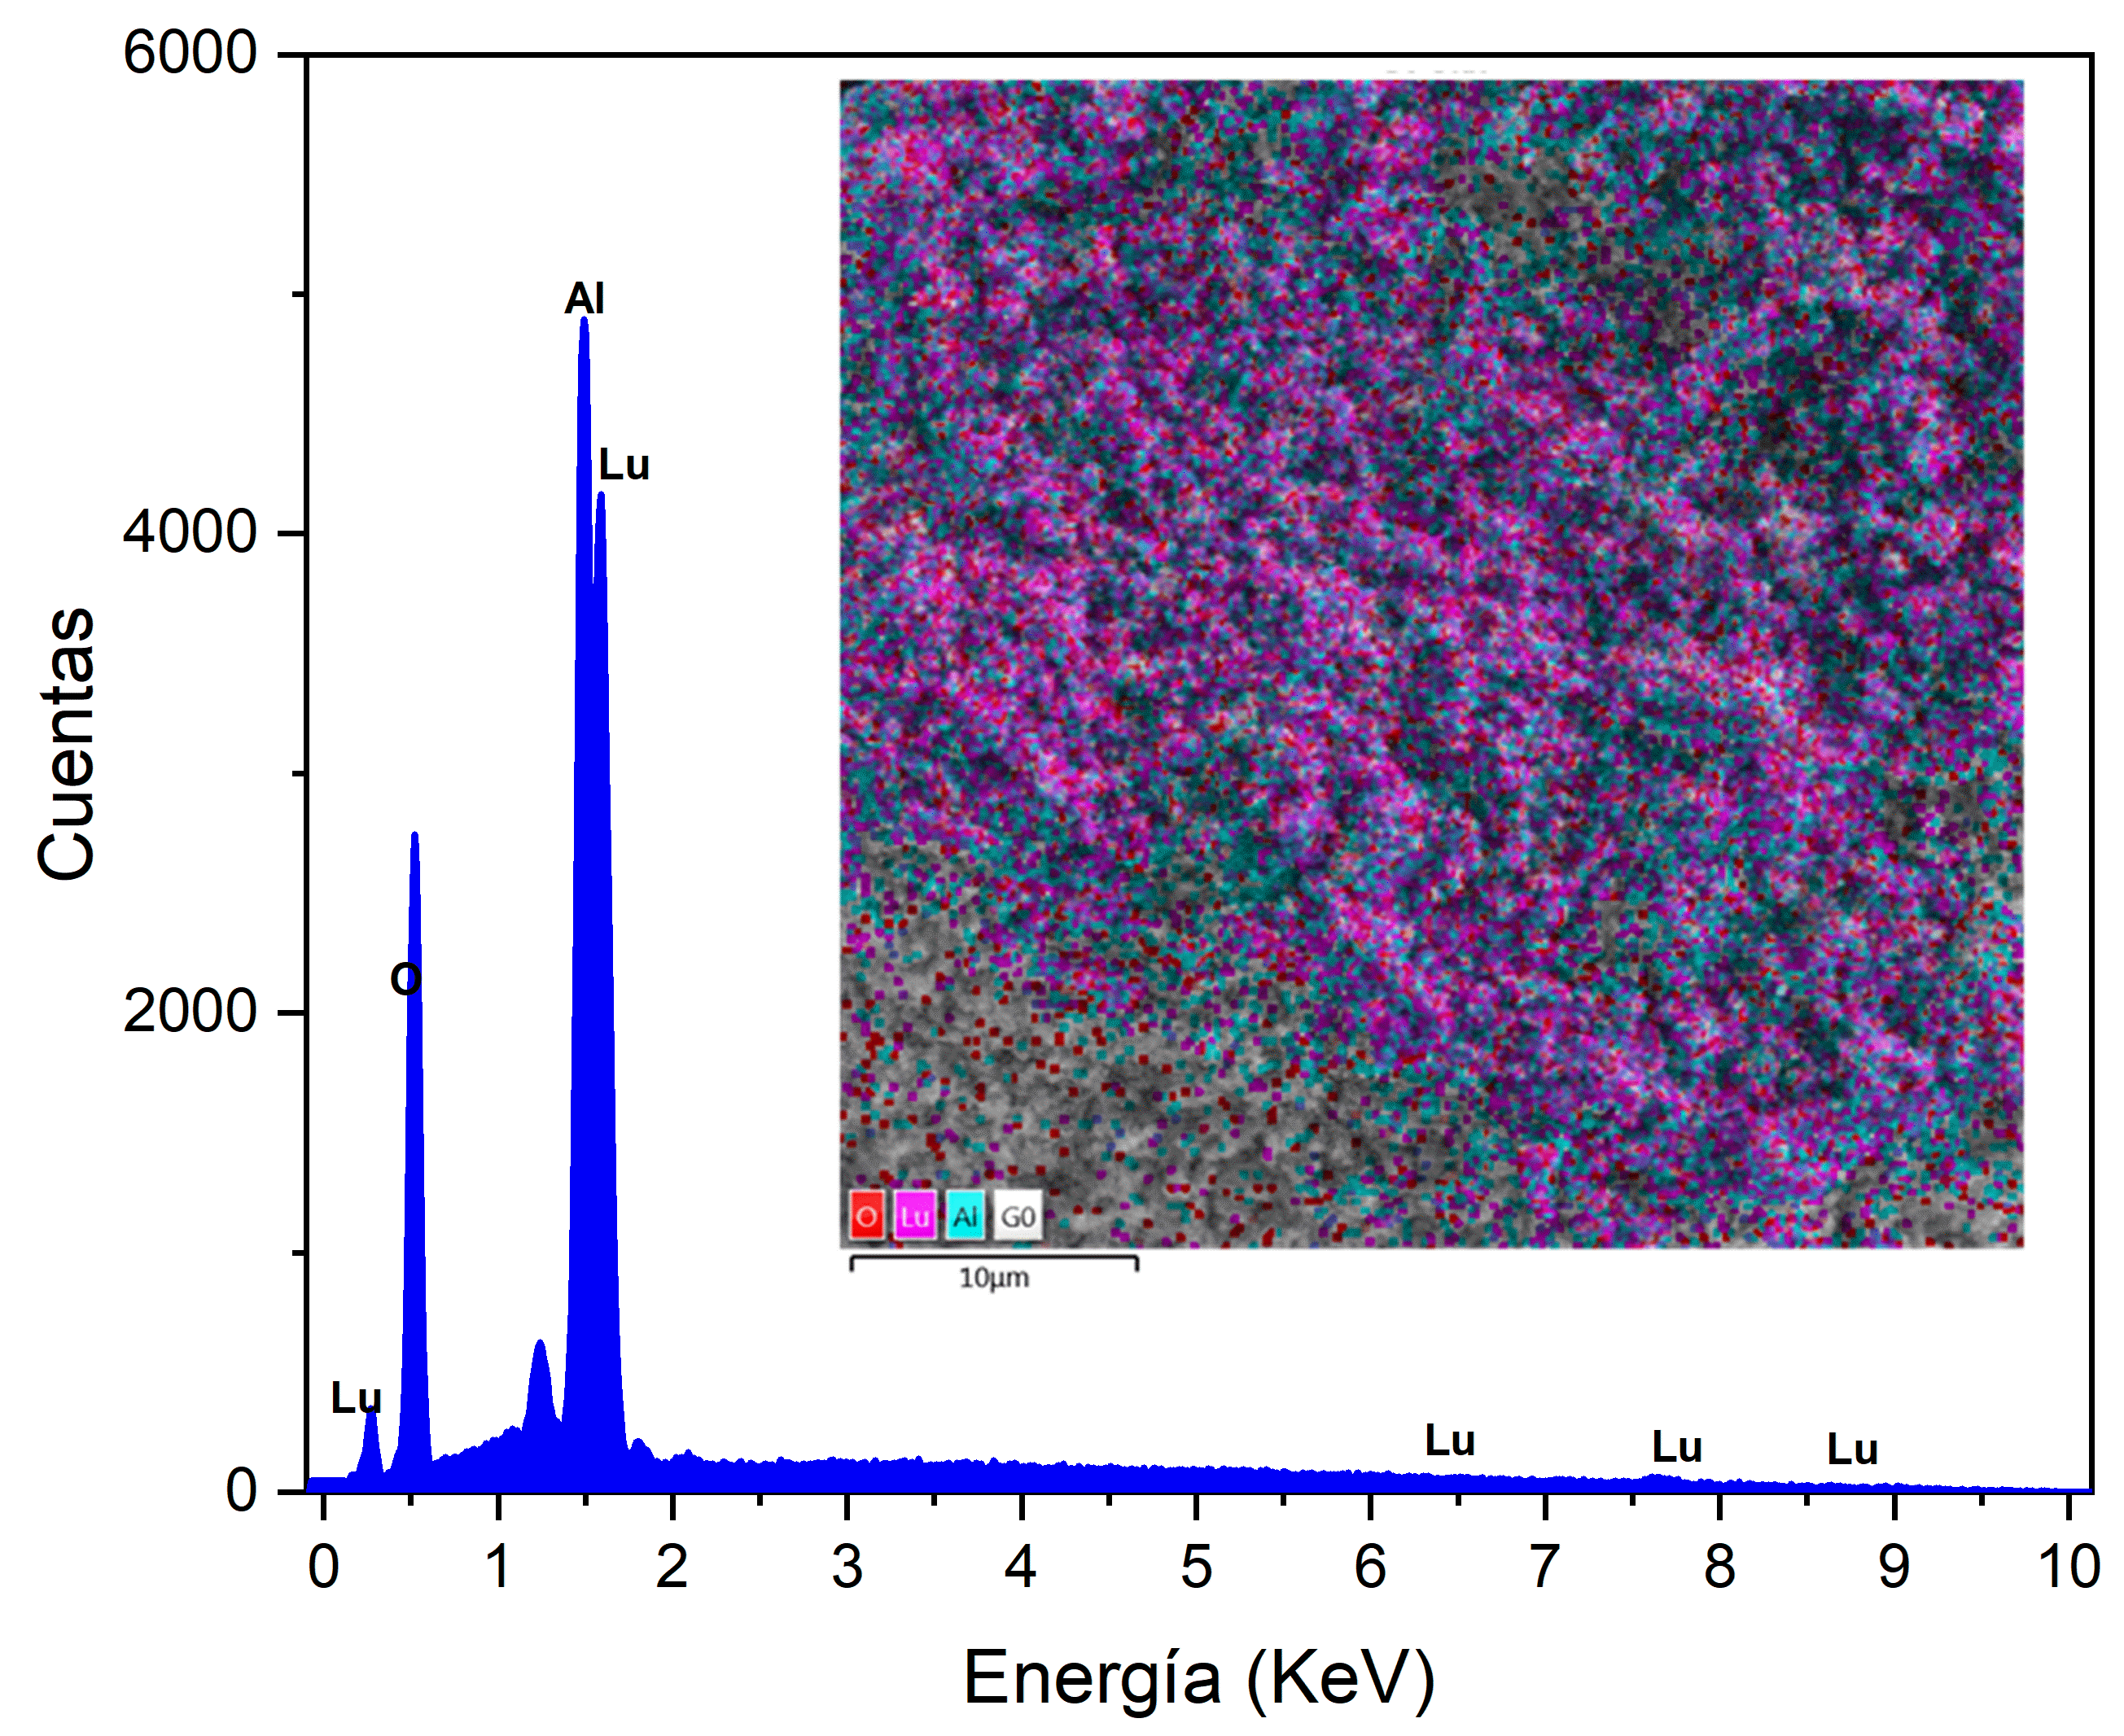
\includegraphics[width=\textwidth]{Anexos/EDXG0.png}%
		\caption{EDX de \ce{Lu_{3.0}Al_{5.0}O12}}\label{fig:edxg0}
	\end{figure}

	\begin{figure}[h]
		\centering%

		\includegraphics[width=\textwidth]{Anexos/EDXG1.png}%
		\caption{EDX de \ce{Lu_{3.0}Al_{4.5}Fe_{0.5}O12}}\label{fig:edxg1}
	\end{figure}

	\begin{figure}[h]
		\centering%

		\includegraphics[width=\textwidth]{Anexos/EDXG5.png}%
		\caption{EDX de \ce{Lu_{3.0}Al_{2.5}Fe_{2.5}O12}}\label{fig:edxg5}
	\end{figure}

	\begin{figure}[h]
		\centering%

		\includegraphics[width=\textwidth]{Anexos/EDXG9.png}%
		\caption{EDX de \ce{Lu_{3.0}Al_{0.5}Fe_{4.5}O12}}\label{fig:edxg9}
	\end{figure}


\end{appendix}
\phantomsection
\addcontentsline{toc}{chapter}{\numberline{}Referencias}

\bibliography{library}
\bibliographystyle{ieeetr}

\end{document}